%% This conference paper was made by Domokos Kiss, G�bor Csorv�si and �kos Nagy, based on
%%
%% bare_conf.tex
%% V1.3
%% 2007/01/11
%% by Michael Shell
%% See:
%% http://www.michaelshell.org/
%% for current contact information.
%%
%% This is a skeleton file demonstrating \textbf{?}the use of IEEEtran.cls
%% (requires IEEEtran.cls version 1.7 or later) with an IEEE conference paper.
%%
%% Support sites:
%% http://www.michaelshell.org/tex/ieeetran/
%% http://www.ctan.org/tex-archive/macros/latex/contrib/IEEEtran/
%% and
%% http://www.ieee.org/

%%*************************************************************************
%% Legal Notice:
%% This code is offered as-is without any warranty either expressed or
%% implied; without even the implied warranty of MERCHANTABILITY or
%% FITNESS FOR A PARTICULAR PURPOSE! 
%% User assumes all risk.
%% In no event shall IEEE or any contributor to this code be liable for
%% any damages or losses, including, but not limited to, incidental,
%% consequential, or any other damages, resulting from the use or misuse
%% of any information contained here.
%%
%% All comments are the opinions of their respective authors and are not
%% necessarily endorsed by the IEEE.
%%
%% This work is distributed under the LaTeX Project Public License (LPPL)
%% ( http://www.latex-project.org/ ) version 1.3, and may be freely used,
%% distributed and modified. A copy of the LPPL, version 1.3, is included
%% in the base LaTeX documentation of all distributions of LaTeX released
%% 2003/12/01 or later.
%% Retain all contribution notices and credits.
%% ** Modified files should be clearly indicated as such, including  **
%% ** renaming them and changing author support contact information. **
%%
%% File list of work: IEEEtran.cls, IEEEtran_HOWTO.pdf, bare_adv.tex,
%%                    bare_conf.tex, bare_jrnl.tex, bare_jrnl_compsoc.tex
%%*************************************************************************

% *** Authors should verify (and, if needed, correct) their LaTeX system  ***
% *** with the testflow diagnostic prior to trusting their LaTeX platform ***
% *** with production work. IEEE's font choices can trigger bugs that do  ***
% *** not appear when using other class files.                            ***
% The testflow support page is at:
% http://www.michaelshell.org/tex/testflow/



% Note that the a4paper option is mainly intended so that authors in
% countries using A4 can easily print to A4 and see how their papers will
% look in print - the typesetting of the document will not typically be
% affected with changes in paper size (but the bottom and side margins will).
% Use the testflow package mentioned above to verify correct handling of
% both paper sizes by the user's LaTeX system.
%
% Also note that the "draftcls" or "draftclsnofoot", not "draft", option
% should be used if it is desired that the figures are to be displayed in
% draft mode.
%
\documentclass[conference]{IEEEtran}
% Add the compsoc option for Computer Society conferences.
%
% If IEEEtran.cls has not been installed into the LaTeX system files,
% manually specify the path to it like:
% \documentclass[conference]{../sty/IEEEtran}





% Some very useful LaTeX packages include:
% (uncomment the ones you want to load)


% *** MISC UTILITY PACKAGES ***
%
%\usepackage{ifpdf}
% Heiko Oberdiek's ifpdf.sty is very useful if you need conditional
% compilation based on whether the output is pdf or dvi.
% usage:
% \ifpdf
%   % pdf code
% \else
%   % dvi code
% \fi
% The latest version of ifpdf.sty can be obtained from:
% http://www.ctan.org/tex-archive/macros/latex/contrib/oberdiek/
% Also, note that IEEEtran.cls V1.7 and later provides a builtin
% \ifCLASSINFOpdf conditional that works the same way.
% When switching from latex to pdflatex and vice-versa, the compiler may
% have to be run twice to clear warning/error messages.






% *** CITATION PACKAGES ***
%
\usepackage{cite}
% cite.sty was written by Donald Arseneau
% V1.6 and later of IEEEtran pre-defines the format of the cite.sty package
% \cite{} output to follow that of IEEE. Loading the cite package will
% result in citation numbers being automatically sorted and properly
% "compressed/ranged". e.g., [1], [9], [2], [7], [5], [6] without using
% cite.sty will become [1], [2], [5]--[7], [9] using cite.sty. cite.sty's
% \cite will automatically add leading space, if needed. Use cite.sty's
% noadjust option (cite.sty V3.8 and later) if you want to turn this off.
% cite.sty is already installed on most LaTeX systems. Be sure and use
% version 4.0 (2003-05-27) and later if using hyperref.sty. cite.sty does
% not currently provide for hyperlinked citations.
% The latest version can be obtained at:
% http://www.ctan.org/tex-archive/macros/latex/contrib/cite/
% The documentation is contained in the cite.sty file itself.






% *** GRAPHICS RELATED PACKAGES ***
%
\ifCLASSINFOpdf
  \usepackage[pdftex]{graphicx}
  % declare the path(s) where your graphic files are
  % \graphicspath{{../pdf/}{../jpeg/}}
  % and their extensions so you won't have to specify these with
  % every instance of \includegraphics
  % \DeclareGraphicsExtensions{.pdf,.jpeg,.png}
\else
  % or other class option (dvipsone, dvipdf, if not using dvips). graphicx
  % will default to the driver specified in the system graphics.cfg if no
  % driver is specified.
  % \usepackage[dvips]{graphicx}
  % declare the path(s) where your graphic files are
  % \graphicspath{{../eps/}}
  % and their extensions so you won't have to specify these with
  % every instance of \includegraphics
  % \DeclareGraphicsExtensions{.eps}
\fi
% graphicx was written by David Carlisle and Sebastian Rahtz. It is
% required if you want graphics, photos, etc. graphicx.sty is already
% installed on most LaTeX systems. The latest version and documentation can
% be obtained at: 
% http://www.ctan.org/tex-archive/macros/latex/required/graphics/
% Another good source of documentation is "Using Imported Graphics in
% LaTeX2e" by Keith Reckdahl which can be found as epslatex.ps or
% epslatex.pdf at: http://www.ctan.org/tex-archive/info/
%
% latex, and pdflatex in dvi mode, support graphics in encapsulated
% postscript (.eps) format. pdflatex in pdf mode supports graphics
% in .pdf, .jpeg, .png and .mps (metapost) formats. Users should ensure
% that all non-photo figures use a vector format (.eps, .pdf, .mps) and
% not a bitmapped formats (.jpeg, .png). IEEE frowns on bitmapped formats
% which can result in "jaggedy"/blurry rendering of lines and letters as
% well as large increases in file sizes.
%
% You can find documentation about the pdfTeX application at:
% http://www.tug.org/applications/pdftex





% *** MATH PACKAGES ***
%
\usepackage[cmex10]{amsmath}
% A popular package from the American Mathematical Society that provides
% many useful and powerful commands for dealing with mathematics. If using
% it, be sure to load this package with the cmex10 option to ensure that
% only type 1 fonts will utilized at all point sizes. Without this option,
% it is possible that some math symbols, particularly those within
% footnotes, will be rendered in bitmap form which will result in a
% document that can not be IEEE Xplore compliant!
%
% Also, note that the amsmath package sets \interdisplaylinepenalty to 10000
% thus preventing page breaks from occurring within multiline equations. Use:
\interdisplaylinepenalty=2500
% after loading amsmath to restore such page breaks as IEEEtran.cls normally
% does. amsmath.sty is already installed on most LaTeX systems. The latest
% version and documentation can be obtained at:
% http://www.ctan.org/tex-archive/macros/latex/required/amslatex/math/


\usepackage{amsfonts}
\usepackage{amsthm}


% *** SPECIALIZED LIST PACKAGES ***
%
%\usepackage{algorithmic}
% algorithmic.sty was written by Peter Williams and Rogerio Brito.
% This package provides an algorithmic environment fo describing algorithms.
% You can use the algorithmic environment in-text or within a figure
% environment to provide for a floating algorithm. Do NOT use the algorithm
% floating environment provided by algorithm.sty (by the same authors) or
% algorithm2e.sty (by Christophe Fiorio) as IEEE does not use dedicated
% algorithm float types and packages that provide these will not provide
% correct IEEE style captions. The latest version and documentation of
% algorithmic.sty can be obtained at:
% http://www.ctan.org/tex-archive/macros/latex/contrib/algorithms/
% There is also a support site at:
% http://algorithms.berlios.de/index.html
% Also of interest may be the (relatively newer and more customizable)
% algorithmicx.sty package by Szasz Janos:
% http://www.ctan.org/tex-archive/macros/latex/contrib/algorithmicx/

\usepackage{algpseudocode}
\usepackage{algorithm}


% *** ALIGNMENT PACKAGES ***
%
\usepackage{array}
% Frank Mittelbach's and David Carlisle's array.sty patches and improves
% the standard LaTeX2e array and tabular environments to provide better
% appearance and additional user controls. As the default LaTeX2e table
% generation code is lacking to the point of almost being broken with
% respect to the quality of the end results, all users are strongly
% advised to use an enhanced (at the very least that provided by array.sty)
% set of table tools. array.sty is already installed on most systems. The
% latest version and documentation can be obtained at:
% http://www.ctan.org/tex-archive/macros/latex/required/tools/


%\usepackage{mdwmath}
%\usepackage{mdwtab}
% Also highly recommended is Mark Wooding's extremely powerful MDW tools,
% especially mdwmath.sty and mdwtab.sty which are used to format equations
% and tables, respectively. The MDWtools set is already installed on most
% LaTeX systems. The lastest version and documentation is available at:
% http://www.ctan.org/tex-archive/macros/latex/contrib/mdwtools/


% IEEEtran contains the IEEEeqnarray family of commands that can be used to
% generate multiline equations as well as matrices, tables, etc., of high
% quality.


%\usepackage{eqparbox}
% Also of notable interest is Scott Pakin's eqparbox package for creating
% (automatically sized) equal width boxes - aka "natural width parboxes".
% Available at:
% http://www.ctan.org/tex-archive/macros/latex/contrib/eqparbox/





% *** SUBFIGURE PACKAGES ***
%\usepackage[tight,footnotesize]{subfigure}
% subfigure.sty was written by Steven Douglas Cochran. This package makes it
% easy to put subfigures in your figures. e.g., "Figure 1a and 1b". For IEEE
% work, it is a good idea to load it with the tight package option to reduce
% the amount of white space around the subfigures. subfigure.sty is already
% installed on most LaTeX systems. The latest version and documentation can
% be obtained at:
% http://www.ctan.org/tex-archive/obsolete/macros/latex/contrib/subfigure/
% subfigure.sty has been superceeded by subfig.sty.



%\usepackage[caption=false]{caption}
%\usepackage[font=footnotesize]{subfig}
% subfig.sty, also written by Steven Douglas Cochran, is the modern
% replacement for subfigure.sty. However, subfig.sty requires and
% automatically loads Axel Sommerfeldt's caption.sty which will override
% IEEEtran.cls handling of captions and this will result in nonIEEE style
% figure/table captions. To prevent this problem, be sure and preload
% caption.sty with its "caption=false" package option. This is will preserve
% IEEEtran.cls handing of captions. Version 1.3 (2005/06/28) and later 
% (recommended due to many improvements over 1.2) of subfig.sty supports
% the caption=false option directly:
\usepackage[caption=false,font=footnotesize]{subfig}
%
% The latest version and documentation can be obtained at:
% http://www.ctan.org/tex-archive/macros/latex/contrib/subfig/
% The latest version and documentation of caption.sty can be obtained at:
% http://www.ctan.org/tex-archive/macros/latex/contrib/caption/




% *** FLOAT PACKAGES ***
%
%\usepackage{fixltx2e}
% fixltx2e, the successor to the earlier fix2col.sty, was written by
% Frank Mittelbach and David Carlisle. This package corrects a few problems
% in the LaTeX2e kernel, the most notable of which is that in current
% LaTeX2e releases, the ordering of single and double column floats is not
% guaranteed to be preserved. Thus, an unpatched LaTeX2e can allow a
% single column figure to be placed prior to an earlier double column
% figure. The latest version and documentation can be found at:
% http://www.ctan.org/tex-archive/macros/latex/base/



%\usepackage{stfloats}
% stfloats.sty was written by Sigitas Tolusis. This package gives LaTeX2e
% the ability to do double column floats at the bottom of the page as well
% as the top. (e.g., "\begin{figure*}[!b]" is not normally possible in
% LaTeX2e). It also provides a command:
%\fnbelowfloat
% to enable the placement of footnotes below bottom floats (the standard
% LaTeX2e kernel puts them above bottom floats). This is an invasive package
% which rewrites many portions of the LaTeX2e float routines. It may not work
% with other packages that modify the LaTeX2e float routines. The latest
% version and documentation can be obtained at:
% http://www.ctan.org/tex-archive/macros/latex/contrib/sttools/
% Documentation is contained in the stfloats.sty comments as well as in the
% presfull.pdf file. Do not use the stfloats baselinefloat ability as IEEE
% does not allow \baselineskip to stretch. Authors submitting work to the
% IEEE should note that IEEE rarely uses double column equations and
% that authors should try to avoid such use. Do not be tempted to use the
% cuted.sty or midfloat.sty packages (also by Sigitas Tolusis) as IEEE does
% not format its papers in such ways.





% *** PDF, URL AND HYPERLINK PACKAGES ***
%
%\usepackage{url}
% url.sty was written by Donald Arseneau. It provides better support for
% handling and breaking URLs. url.sty is already installed on most LaTeX
% systems. The latest version can be obtained at:
% http://www.ctan.org/tex-archive/macros/latex/contrib/misc/
% Read the url.sty source comments for usage information. Basically,
% \url{my_url_here}.





% *** Do not adjust lengths that control margins, column widths, etc. ***
% *** Do not use packages that alter fonts (such as pslatex).         ***
% There should be no need to do such things with IEEEtran.cls V1.6 and later.
% (Unless specifically asked to do so by the journal or conference you plan
% to submit to, of course. )


% Definition of new commands
\providecommand{\abs}[1]{\lvert#1\rvert}
\providecommand{\CCS}{C^*CS}
\providecommand{\ccS}{c\bar{c}S}
\providecommand{\qone}{\tilde{q}_I}
\providecommand{\qonek}{\tilde{q}_{I,k}}
\providecommand{\qonesol}{\tilde{q}_{I,k_{sol}}}
\providecommand{\xone}{\tilde{x}_I}
\providecommand{\yone}{\tilde{y}_I}
\providecommand{\thetaone}{\tilde{\theta}_I}
\providecommand{\xonek}{\tilde{x}_{I,k}}
\providecommand{\yonek}{\tilde{y}_{I,k}}
\providecommand{\thetaonek}{\tilde{\theta}_{I,k}}
\providecommand{\qtwo}{\tilde{q}_G}
\providecommand{\qtwok}{\tilde{q}_{G,k}}
\providecommand{\qtwosol}{\tilde{q}_{G,k_{sol}}}
\providecommand{\xtwo}{\tilde{x}_G}
\providecommand{\ytwo}{\tilde{y}_G}
\providecommand{\xtwok}{\tilde{x}_{G,k}}
\providecommand{\ytwok}{\tilde{y}_{G,k}}
\providecommand{\thetatwo}{\tilde{\theta}_G}
\providecommand{\thetatwok}{\tilde{\theta}_{G,k}}
\providecommand{\rhoone}{\rho_{I,\tilde{I}}}
\providecommand{\rhotwo}{\rho_{\tilde{I},\tilde{G}}}
\providecommand{\rhotwofirst}{\rho_{I,\tilde{G}}}
\providecommand{\sone}{s_{I,\tilde{I}}}
\providecommand{\stwo}{s_{\tilde{I},\tilde{G}}}
\providecommand{\sthree}{s_{\tilde{G},G}}
\providecommand{\sonek}{s_{I,\tilde{I},k}}
\providecommand{\stwok}{s_{\tilde{I},\tilde{G},k}}
\providecommand{\sthreek}{s_{\tilde{G},G,k}}
\providecommand{\soneksol}{s_{I,\tilde{I},k_{sol}}}
\providecommand{\stwoksol}{s_{\tilde{I},\tilde{G},k_{sol}}}
\providecommand{\sthreeksol}{s_{\tilde{G},G,k_{sol}}}



% correct bad hyphenation here
\hyphenation{op-tical net-works semi-conduc-tor}





\begin{document}
%
% paper title
% can use linebreaks \\ within to get better formatting as desired
\title{A Planning Method to Obtain Good Quality Paths for Autonomous Cars}


% author names and affiliations
% use a multiple column layout for up to three different
% affiliations
\author{\IEEEauthorblockN{Domokos Kiss, G\'abor Csorv\'asi and \'Akos Nagy}
\IEEEauthorblockA{Department of Automation and Applied Informatics\\ 
Budapest University of Technology and Economics\\
domokos.kiss@aut.bme.hu, gabor.csorvasi@aut.bme.hu, akos.nagy@aut.bme.hu}}

% conference papers do not typically use \thanks and this command
% is locked out in conference mode. If really needed, such as for
% the acknowledgment of grants, issue a \IEEEoverridecommandlockouts
% after \documentclass

% for over three affiliations, or if they all won't fit within the width
% of the page, use this alternative format:
% 
%\author{\IEEEauthorblockN{Michael Shell\IEEEauthorrefmark{1},
%Homer Simpson\IEEEauthorrefmark{2},
%James Kirk\IEEEauthorrefmark{3}, 
%Montgomery Scott\IEEEauthorrefmark{3} and
%Eldon Tyrell\IEEEauthorrefmark{4}}
%\IEEEauthorblockA{\IEEEauthorrefmark{1}School of Electrical and Computer Engineering\\
%Georgia Institute of Technology,
%Atlanta, Georgia 30332--0250\\ Email: see http://www.michaelshell.org/contact.html}
%\IEEEauthorblockA{\IEEEauthorrefmark{2}Twentieth Century Fox, Springfield, USA\\
%Email: homer@thesimpsons.com}
%\IEEEauthorblockA{\IEEEauthorrefmark{3}Starfleet Academy, San Francisco, California 96678-2391\\
%Telephone: (800) 555--1212, Fax: (888) 555--1212}
%\IEEEauthorblockA{\IEEEauthorrefmark{4}Tyrell Inc., 123 Replicant Street, Los Angeles, California 90210--4321}}




% use for special paper notices
%\IEEEspecialpapernotice{(Invited Paper)}




% make the title area
\maketitle


\begin{abstract}
%\boldmath
Path planning among obstacles for nonholonomic systems is a widely researched area nowadays, but it is still one of the most challenging problems in autonomous navigation. We have recently presented a rapidly exploring random tree based global planner (RTR) and a steering method (C*CS) for car-like vehicles, which uses circular and straight movements. With the aid of these two methods it is possible to obtain a feasible path, even in narrow spaces and in situations requiring non-trivial maneuvers. This paper presents an improved solution for environments, where not all obstacles are known at the beginning and these are discovered during the motion of the robot. We also introduce an extension to the presented algorithm to achieve paths of better quality, i.e. more similar to a reasonable path generated by a human driver.

\end{abstract}
% IEEEtran.cls defaults to using nonbold math in the Abstract.
% This preserves the distinction between vectors and scalars. However,
% if the conference you are submitting to favors bold math in the abstract,
% then you can use LaTeX's standard command \boldmath at the very start
% of the abstract to achieve this. Many IEEE journals/conferences frown on
% math in the abstract anyway.

% no keywords



% For peer review papers, you can put extra information on the cover
% page as needed:
% \ifCLASSOPTIONpeerreview
% \begin{center} \bfseries EDICS Category: 3-BBND \end{center}
% \fi
%
% For peerreview papers, this IEEEtran command inserts a page break and
% creates the second title. It will be ignored for other modes.
\IEEEpeerreviewmaketitle





\section{Introduction}
\label{sec:intro}
Driving support systems (e.g. parking assistant, collision avoidance) are increasingly widespread nowadays. In some application these intelligent systems plan the path for the vehicle from a start position to the desired goal position. Due to the presence of obstacles this is not an easy task at all. Kinematic constraints of the vehicle are also make path planning difficult. Cars have nonholonomic constraints which cause difficulties in the control of such robots, even in the absence of obstacles. These constraints cause that a car can only move in the direction of its heading (forwards or backwards) and that the turning radius is lower bounded. For this reason parallel parking with a car is relatively difficult.

From the perspective of motion planning, any robot can be described by its \emph{configuration}. For example, the configuration of a rigid mobile robot moving in a planar workspace $\mathcal{W} \subset \mathbb{R}^2$ can be given by $q = (x, y, \theta)$, a vector of its position and orientation in the configuration space $\mathcal{C}$. The set of not allowed configurations (e.g.\ because of collision with obstacles) is called the configuration space obstacle $\mathcal{C}_{obs}$, its complement is the free space $\mathcal{C}_{free} = \mathcal{C} \setminus \mathcal{C}_{obs}$.

The paper is organized as follows. A brief overview of path planning methods for autonomous robots are given in Section~\ref{sec:related}. In Section~\ref{sec:RTR_CCS}, we shortly discuss our previously developed $RTR$ and $\CCS$ planning methods and show how these can be applied together to obtain feasible paths in narrow environments. Section~\ref{sec:arm} shows our enhanced method for sampling of the configuration space in the $\CCS$ algorithm. In Section~\ref{sec:static}, we present an extension to our path planning methods in order to generate human like paths. We show a planning strategy for environment, where farther obstacles are not known at the beginning in Section~\ref{sec:dynamic}. Conclusions and directions of future work are summarized in Section~\ref{sec:conclusions}.
\section{Related Work}
\label{sec:related}

Path planning for nonholonomic robots is not trivial even in absence of obstacles in the environment \cite{laumond98robotmotion}. Algorithms that can solve this task are called local planners or steering methods. In case of specific wheeled robots exact methods exist for computing optimal (e.g.\ shortest length) local paths. These include our investigated car-like robot model \cite{reeds90optimal, giordano06nonholonomic_distance}.

However, a useful planning algorithm has to generate paths in the presence of obstacles while taking into account the kinematic constraints of the vehicle as well. To the best of our knowledge, there is no general \emph{optimal} solution available for this problem. Thus generally, if obstacles are present, one should be satisfied with a \emph{feasible} solution which is not necessarily optimal. The majority of planning algorithms delivering a feasible solution can be grouped into two main categories. The first category consists of techniques that approximate a not necessarily feasible but collision-free initial geometric path by a sequence of feasible local paths obtained by a steering method~\cite{laumond94motionplanner}. In this case firstly a primary geometric path is planned which takes the obstacles and the shape of the robot into account, but does not care about the kinematic constraints. In a second phase, this path is iteratively subdivided and the parts are tried to be connected by a steering method. If the geometric path has a nonzero clearance $\varepsilon$ from the obstacles, and the steering method verifies the so called \emph{topological property}, then the approximation succeeds in finite time \cite{laumond98guidelines}.

The second category involves sampling-based roadmap methods, which build a graph in order to capture the topology of $\mathcal{C}_{{free}}$ and use local steering methods to connect the graph nodes. A good survey of sampling-based planning methods can be found in \cite{lavalle06planning_chap5}. The majority of these are based on random sampling of the configuration space. Their popularity arise from the fact that they do not require an explicit representation of $\mathcal{C}_{{obs}}$. These methods proved to be successful in many planning problems, including high-dimensional configuration spaces. For example, the Probabilistic Roadmap Method (PRM)~\cite{kavraki96prm} and the Rapidly exploring Random Trees (RRT)~\cite{lavalle98rrt, lavalle01rrt} algorithms are common sampling based planners. The main idea of it is to incrementally build a search tree starting from the initial configuration in a way that the tree covers the free space rapidly and with gradually increasing resolution. 

\section{The RTR+C*CS Path Planner}
\label{sec:RTR_CCS}

Our global path planner (RTR) and steering method (C*CS) have been presented recently \cite{anagy15sami, gcsorvasi15iccc}. The global path designed by RTR consist of translational motion (T) and turning in place (R). Therefore the resulted path is not feasible for car-like robots, but a good starting point for the steering method, because the path is collision free. Thus this path can be approximated by the C*CS local planner, which uses straight segments and circular arcs of lower bounded (but not necessary minimal) radii. The purpose of the approximation is to eliminate in-place turns while avoiding collisions, since these are not feasible for car-like robots.

\subsection{RTR Global Planner}
\label{sec:RTR}

The RTR planner is based on the well-known Rapidly exploring Random
Trees (RRT) algorithm \cite{dkiss14csit}. RTR is similar to a bidirectional RRT  method, because it also builds two tree from the start and goal configuration (\emph{start tree}, \emph{goal tree}). However, the phases (sampling, vertex selection and extension) of the RTR planner are different from RRT. 

The first difference to RRT can be found in the sampling step. It returns a guiding position $p_G$ instead of a configuration, which can be treated as a one-dimensional continuous set of configurations, from which any element can
serve as local goal in the tree extension step. The vertex selection step returns the configuration in the existing tree which has the smallest \emph{position} distance to $p_G$. This step uses a simple Euclidean metric, hence no special configuration space metrics are needed.

The main difference to the RRT method can be found in the tree extension step. It performs some primitive rotate--translate motion pairs, guided by $p_G$. A rotation is applied to reach the orientation pointing to $p_G$, and a consecutive translation is performed in both forward and backward directions until the first collision. If a collision occurs during the rotation, the rotation is tried again in the other turning direction. An example for the resulting RTR-path can be seen in \figurename~\ref{fig:RTR_example}, the two trees are depicted as well by different colors.

\begin{figure}[tb]
	\centering
		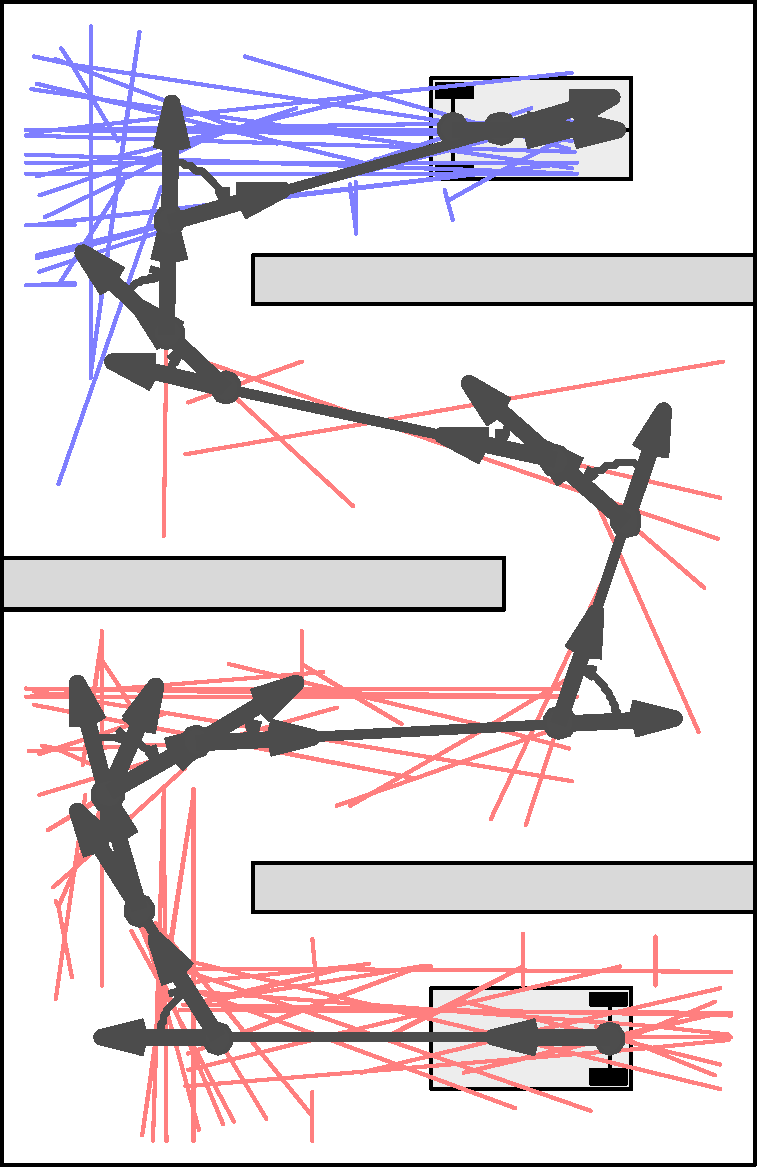
\includegraphics[width=0.5\columnwidth]{.//figures/scenario_RTR.pdf}
	\caption{A result of the RTR planner through a narrow corridor}
	\label{fig:RTR_example}
\end{figure}

\subsection{C*CS Steering Method}
\label{sec:CCS}

The main idea behind the $C\text{*}CS$ local planner it to use circular and straight movements as path primitives \cite{dkiss13aacs, dkiss14iccc}. With the help of these primitives we can arrive from a $q_I$ initial configuration to any $q_G$ goal. To simplify the notation we will use the letter $C$ for the circular arcs and $S$ for the straight segments in the sequel. It can be easily show that without taking into account the curvature bound of a car-like robot and assume that $\theta_I \neq 0$ the goal configuration can be reached with a $CS$ pair as follows. With a tangential arc we turn to an intermediate goal $\tilde{q_G}$ which is in the line of the $q_G$ ($C$). After that only a final straight segment is needed to arrive in the goal ($S$).

\begin{figure}[tb]
	\centering
		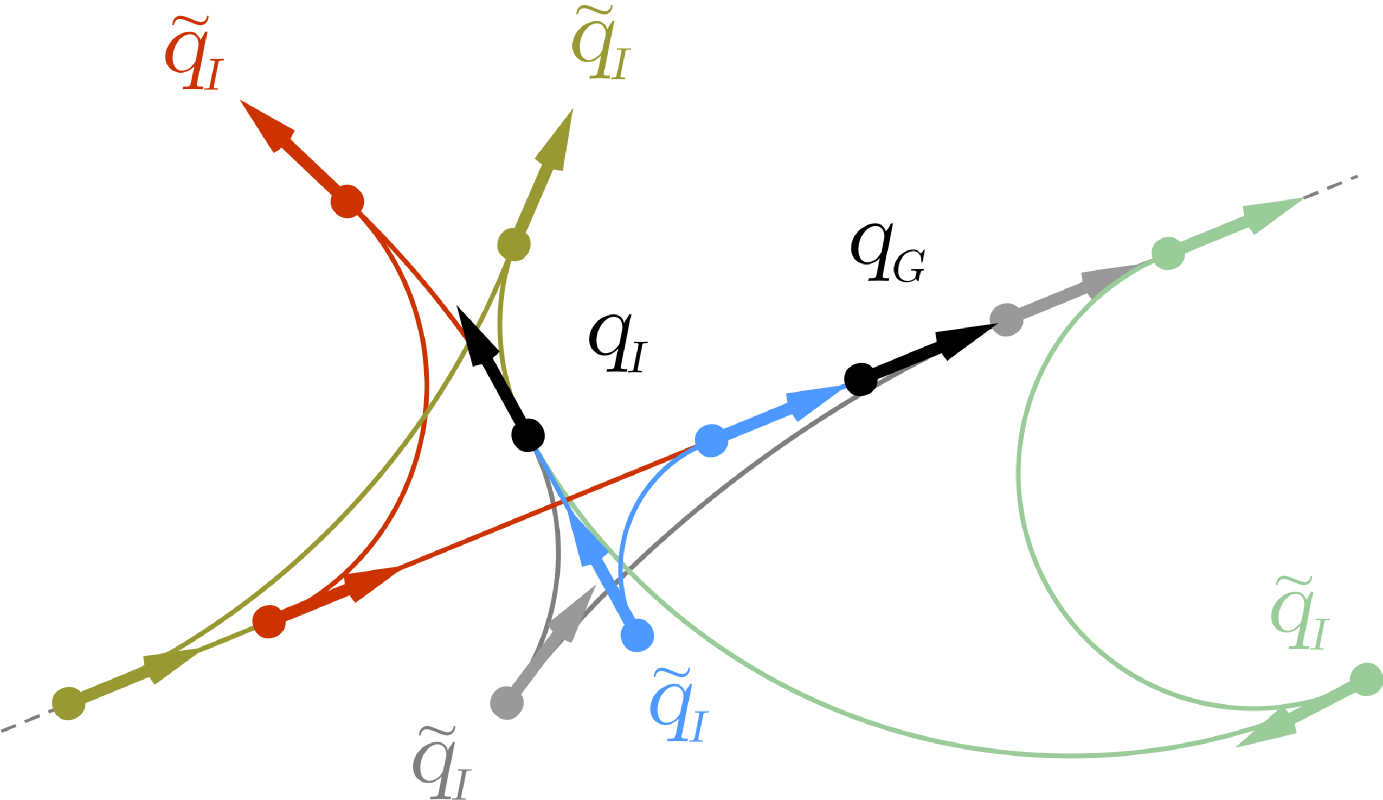
\includegraphics[width=0.8\columnwidth]{.//figures/CCS_example.png}
	\caption{There are many $\CCS$ paths between two configurations}
	\label{fig:CCS_example}
\end{figure}

Unfortunately if the radius of the tangential arc is smaller than the minimal turning radius of the car or it is initially parallel to the line of the goal no feasible path can be found. To help that an intermediate $\tilde{q_I}$ configuration has to be reached where a feasible path is given. It is shown that we have infinitely many possibility to choose one of this intermediate configuration.

The set of configurations, which is reachable from the initial configuration, is called Arc Reachable Manifold (ARM \cite{minguez09extending}) Since this set contains both $C$ and $S$ segments we denote this with $C\text{*}$, where it stands for ``a circular arc that can have zero curvature'' thus $C\text{*}CS$ is a shorthand for both $CCS$ and $SCS$ paths.

\section{Improvements in Sampling Phase}
\label{sec:arm}

Among obstacles the property of infinite solutions is useful, thus there is more possibilities to find a feasible path, and there is a freedom to choose one of the ``prettiest'' solution as well. Although in the implementation we have to use a form of sampling method. Naturally if the sample size is bigger, the calculation takes more time, but if only a few sample is taken the possible solution can be missed.

In our early implementation we used a Sukharev-grid \cite{lavalle06planning_chap5} based sampling method, but this had more drawbacks. The minimally needed sample size was depended on the actual environment, and a lot of calculation was unnecessary for example in far spaces or at the side of the car which is unreachable for an non-holonomic car-like robot.

Our new method is based on the behaviour of these robots and only the closed environment is sampled. To avoid the unnecessary calculation caused by the unreachable area at the two sides of the robot, we sampled the curvature of the possible circular arcs from $0$ to $\kappa_{max}$, where $\kappa_{max} = \frac{1}{r_{min}}$. Also the distance from the robot is sampled from $0$ to a chosen $d_{max}$. Our results shows that the $d_{max} = 2 \cdot r_{min}$ could be a suitable choice. The first step results tangential circles on both side of the robot and the second step results co-centric circles. The intersections of these circles will be the sample points.

In this way the sample size can be reduced so that the possible solutions are still present. The extra time needed for the calculation of the intersections is relatively small compared to the whole calculation process.

\begin{figure}[tb]
	\centering
		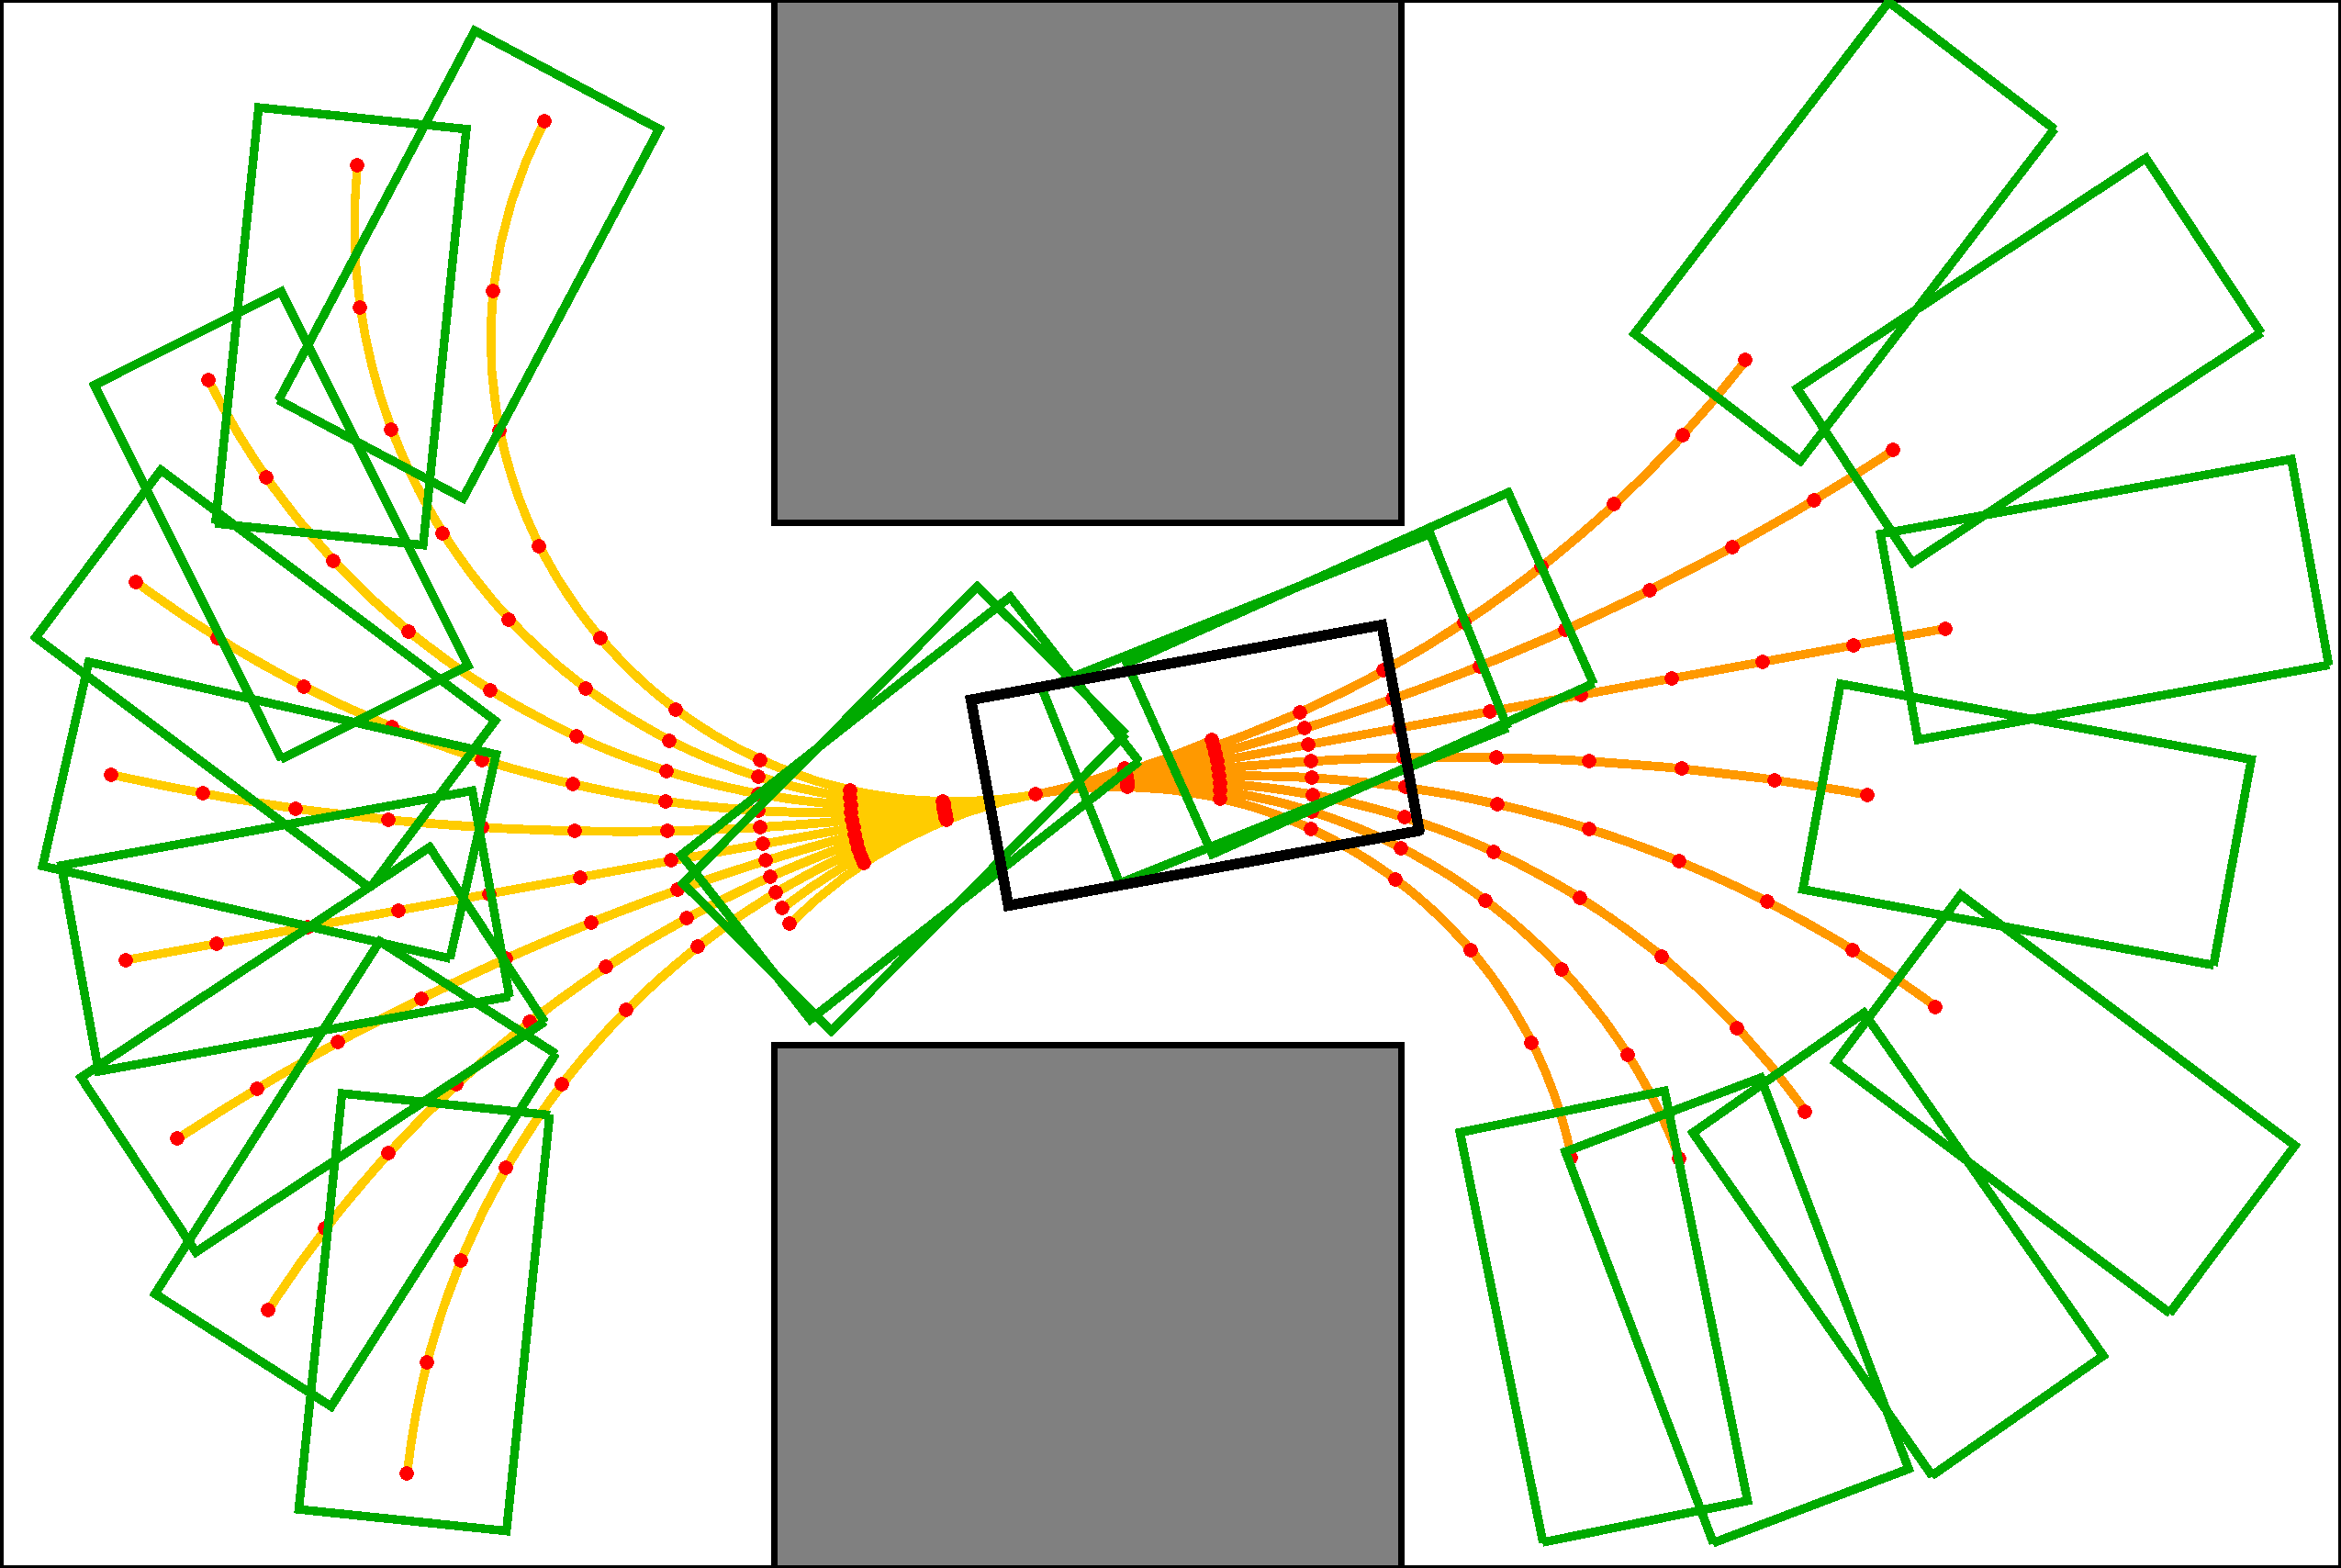
\includegraphics[width=0.90\columnwidth]{.//figures/newARM.pdf}
	\caption{Arc Reachable Manifold in an environment with two obstacles}
	\label{fig:ARM}
\end{figure}

\section{Planning in Dynamic Environment}
\label{sec:dynamic}

Our presented path planning method requires global information about the environment. During collision detection in the RTR and the C*CS algorithm, all obstacles of the environment are checked. In most real situation we do not have global information of the environment or the obstacles of the environment change their position. In both cases the planner algorithm has to be run repeatedly if the environment is changed and the previously generated path is collided.

Consider the following scenario. A 3D laser scanner is located on the top of a car-like robot. This sensor provides the information about the obstacles near the car for the planning algorithm. In our simulation we model this situation with the following way. The robot only detects the obstacles near the current configuration within a fixed radius. In every simulation iteration the program checks whether an obstacle within the sensing radius is discovered. If the new obstacle collide with the path of the robot, the path will be re-planned (see \figurename~\ref{fig:dynamicSim_Phases}). After that, the robot steps forward to the next path configuration. It is important to note, that in our simulation we do not divide obstacles into smaller ones for the sake of simplicity. However, a real 3D laser scanner can provides information about a part of an obstacle.

\begin{figure}[tb]
    \centerline{
    \subfloat[]{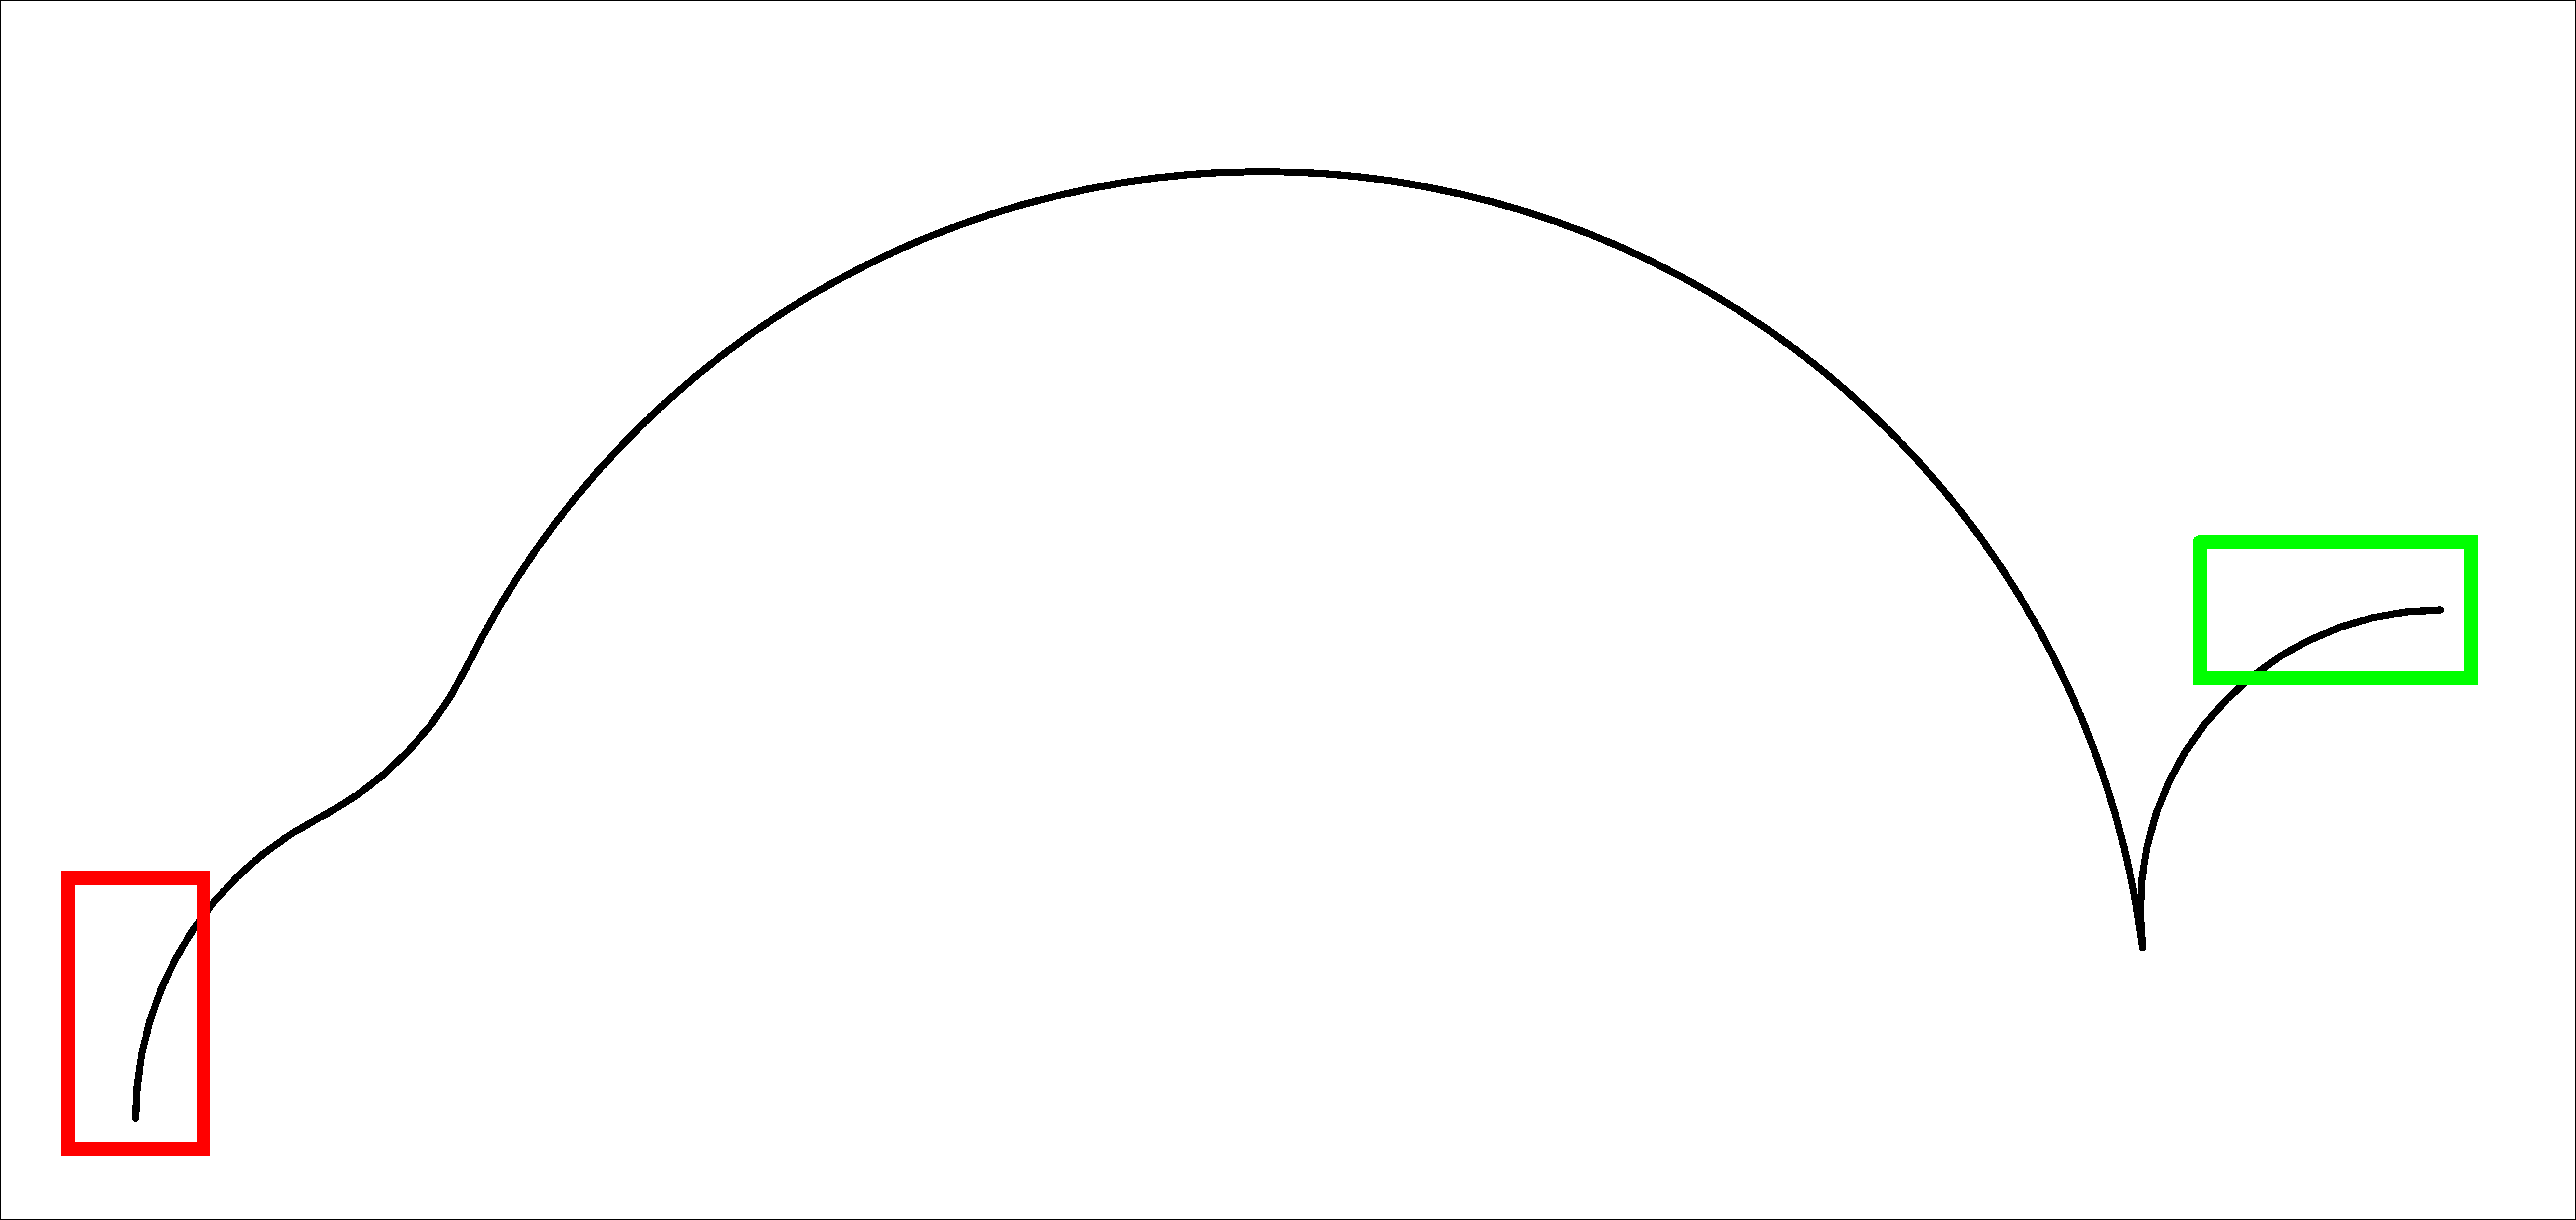
\includegraphics[height=0.35\columnwidth]{.//figures/DynamicSim/plannedPath0N.pdf}
    \label{subfig:phase0}}}
    \centerline{
    \subfloat[]{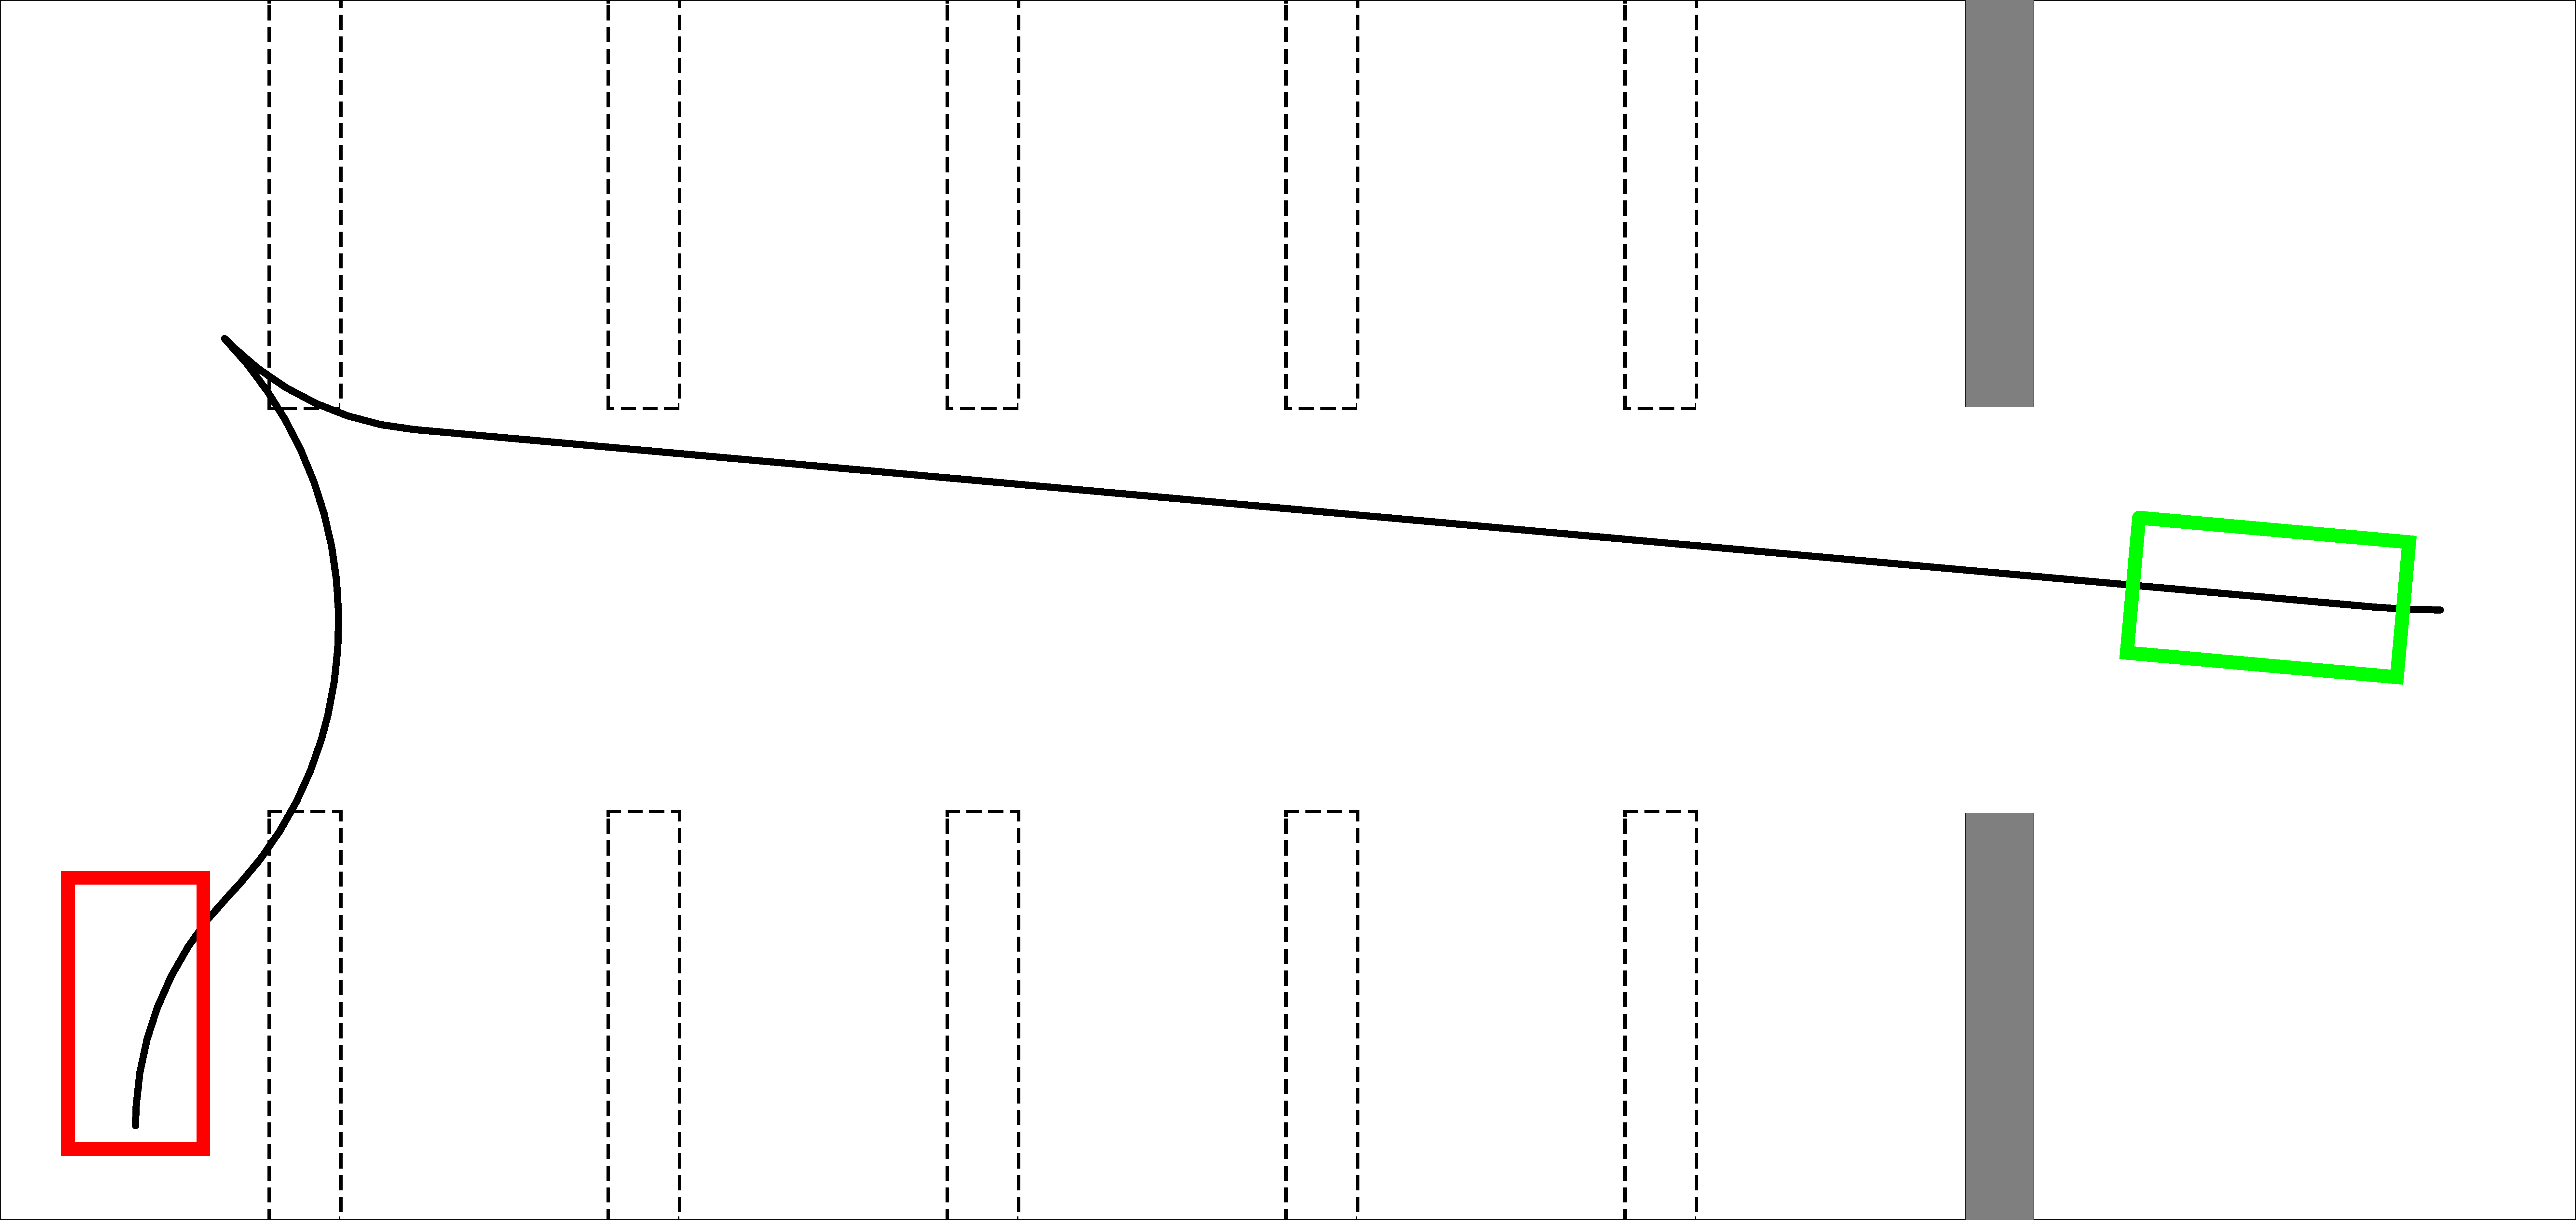
\includegraphics[height=0.35\columnwidth]{.//figures/DynamicSim/plannedPath2N.pdf}
    \label{subfig:phase1}}}
    \centerline{
    \subfloat[]{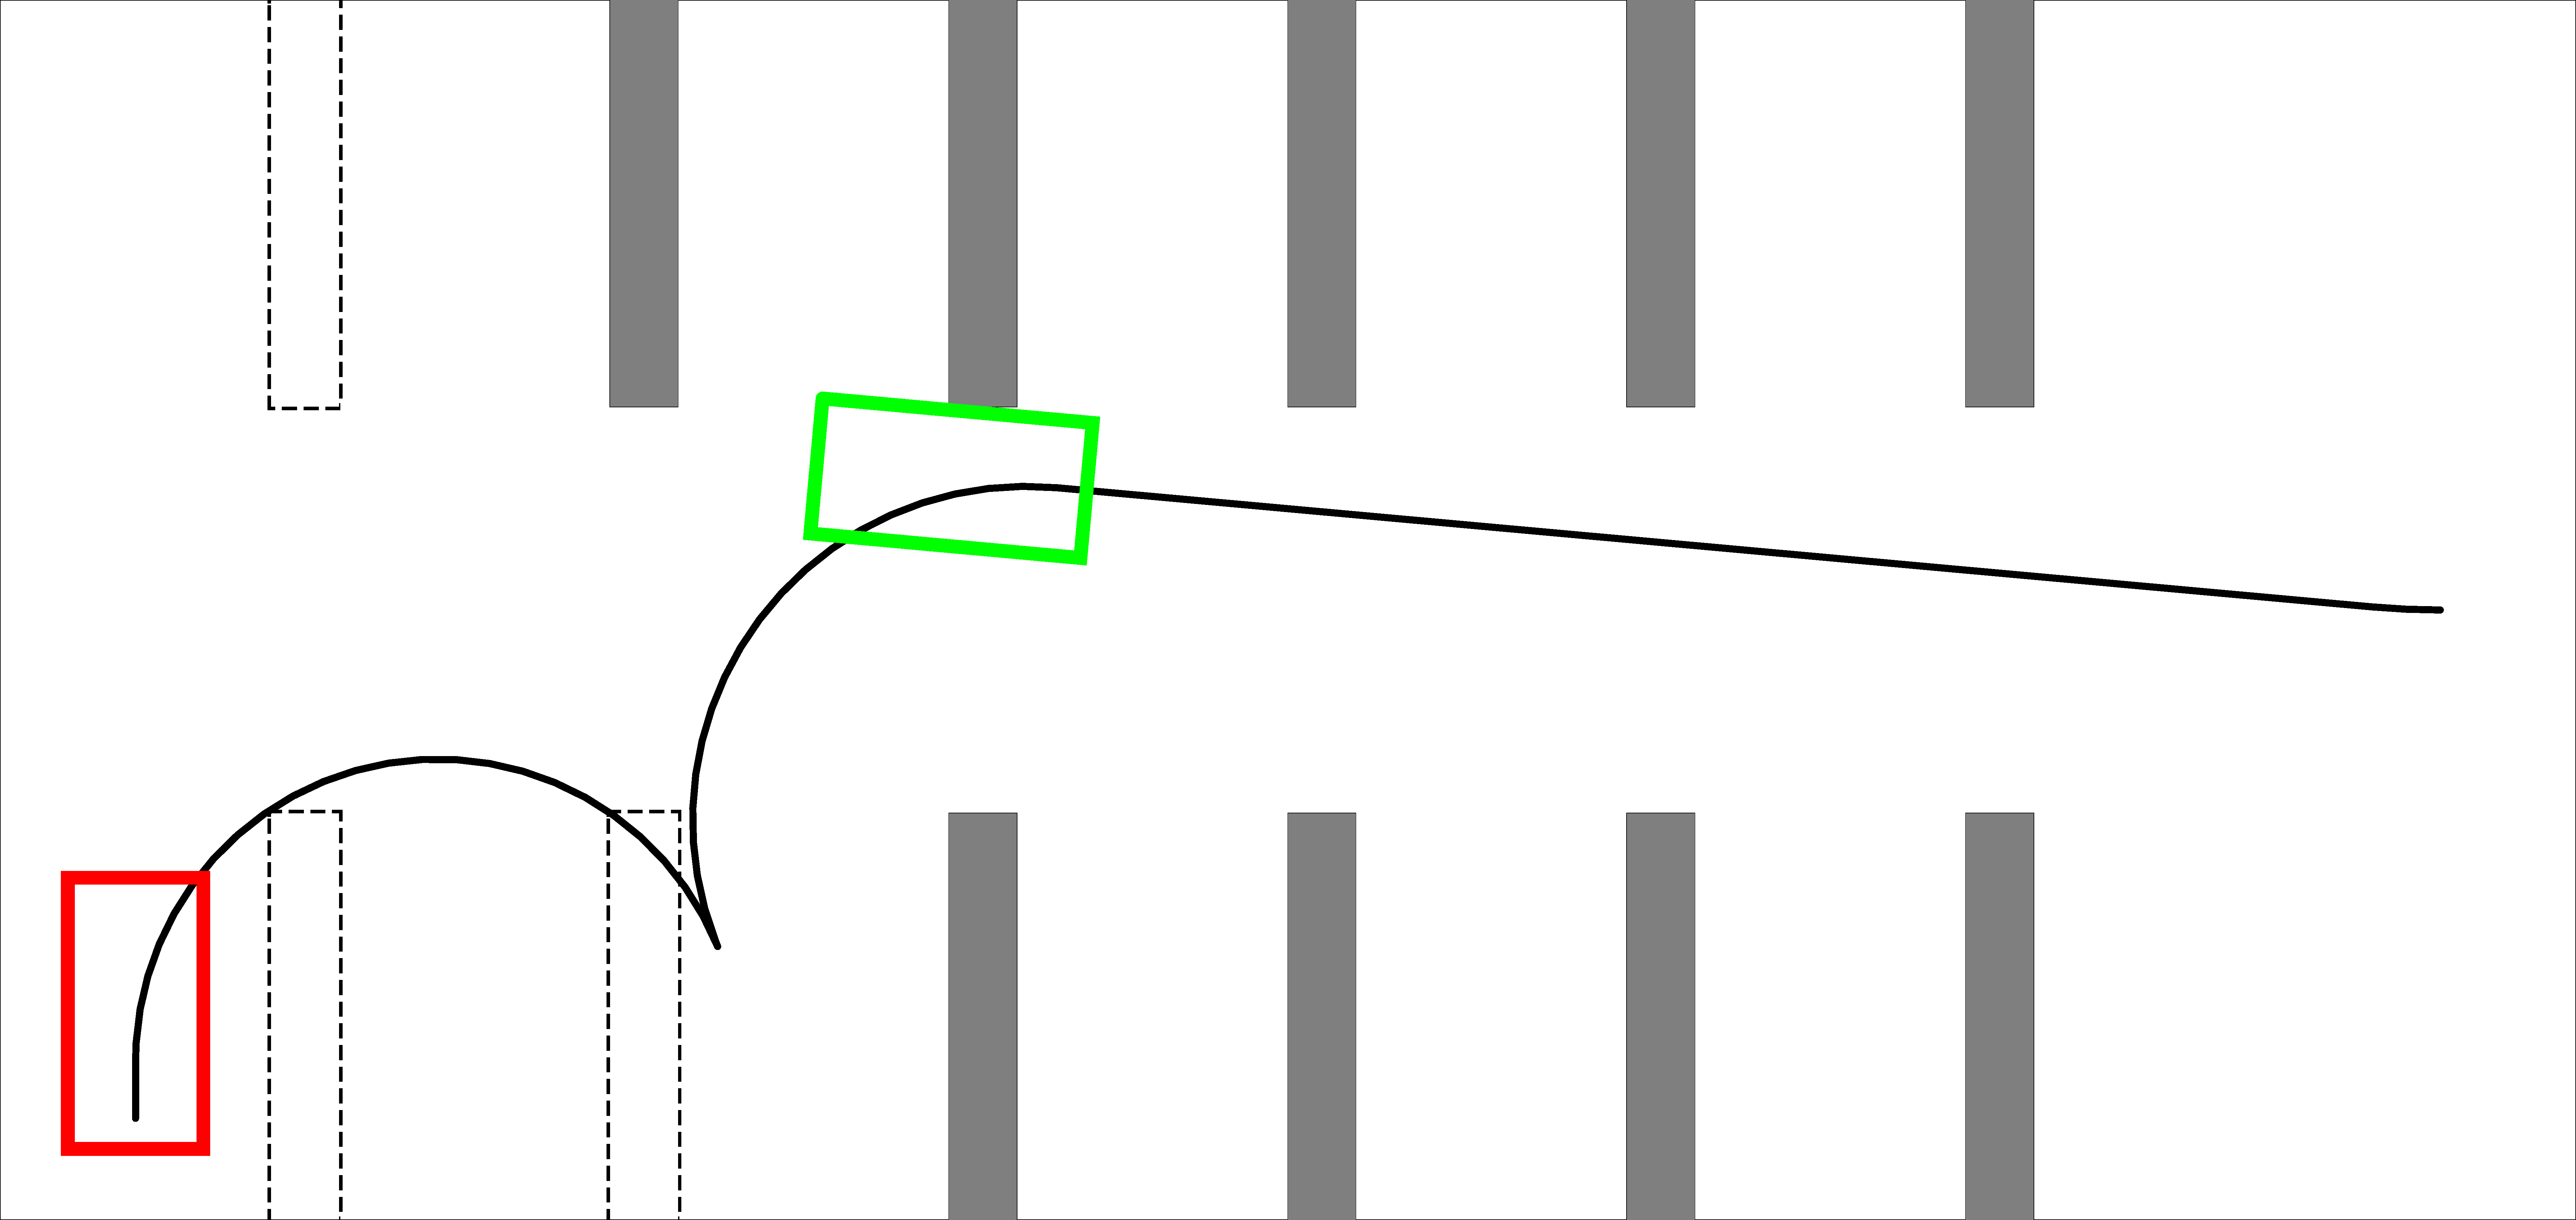
\includegraphics[height=0.35\columnwidth]{.//figures/DynamicSim/plannedPath41N.pdf}
    \label{subfig:phase3}}}    
    \centerline{
    \subfloat[]{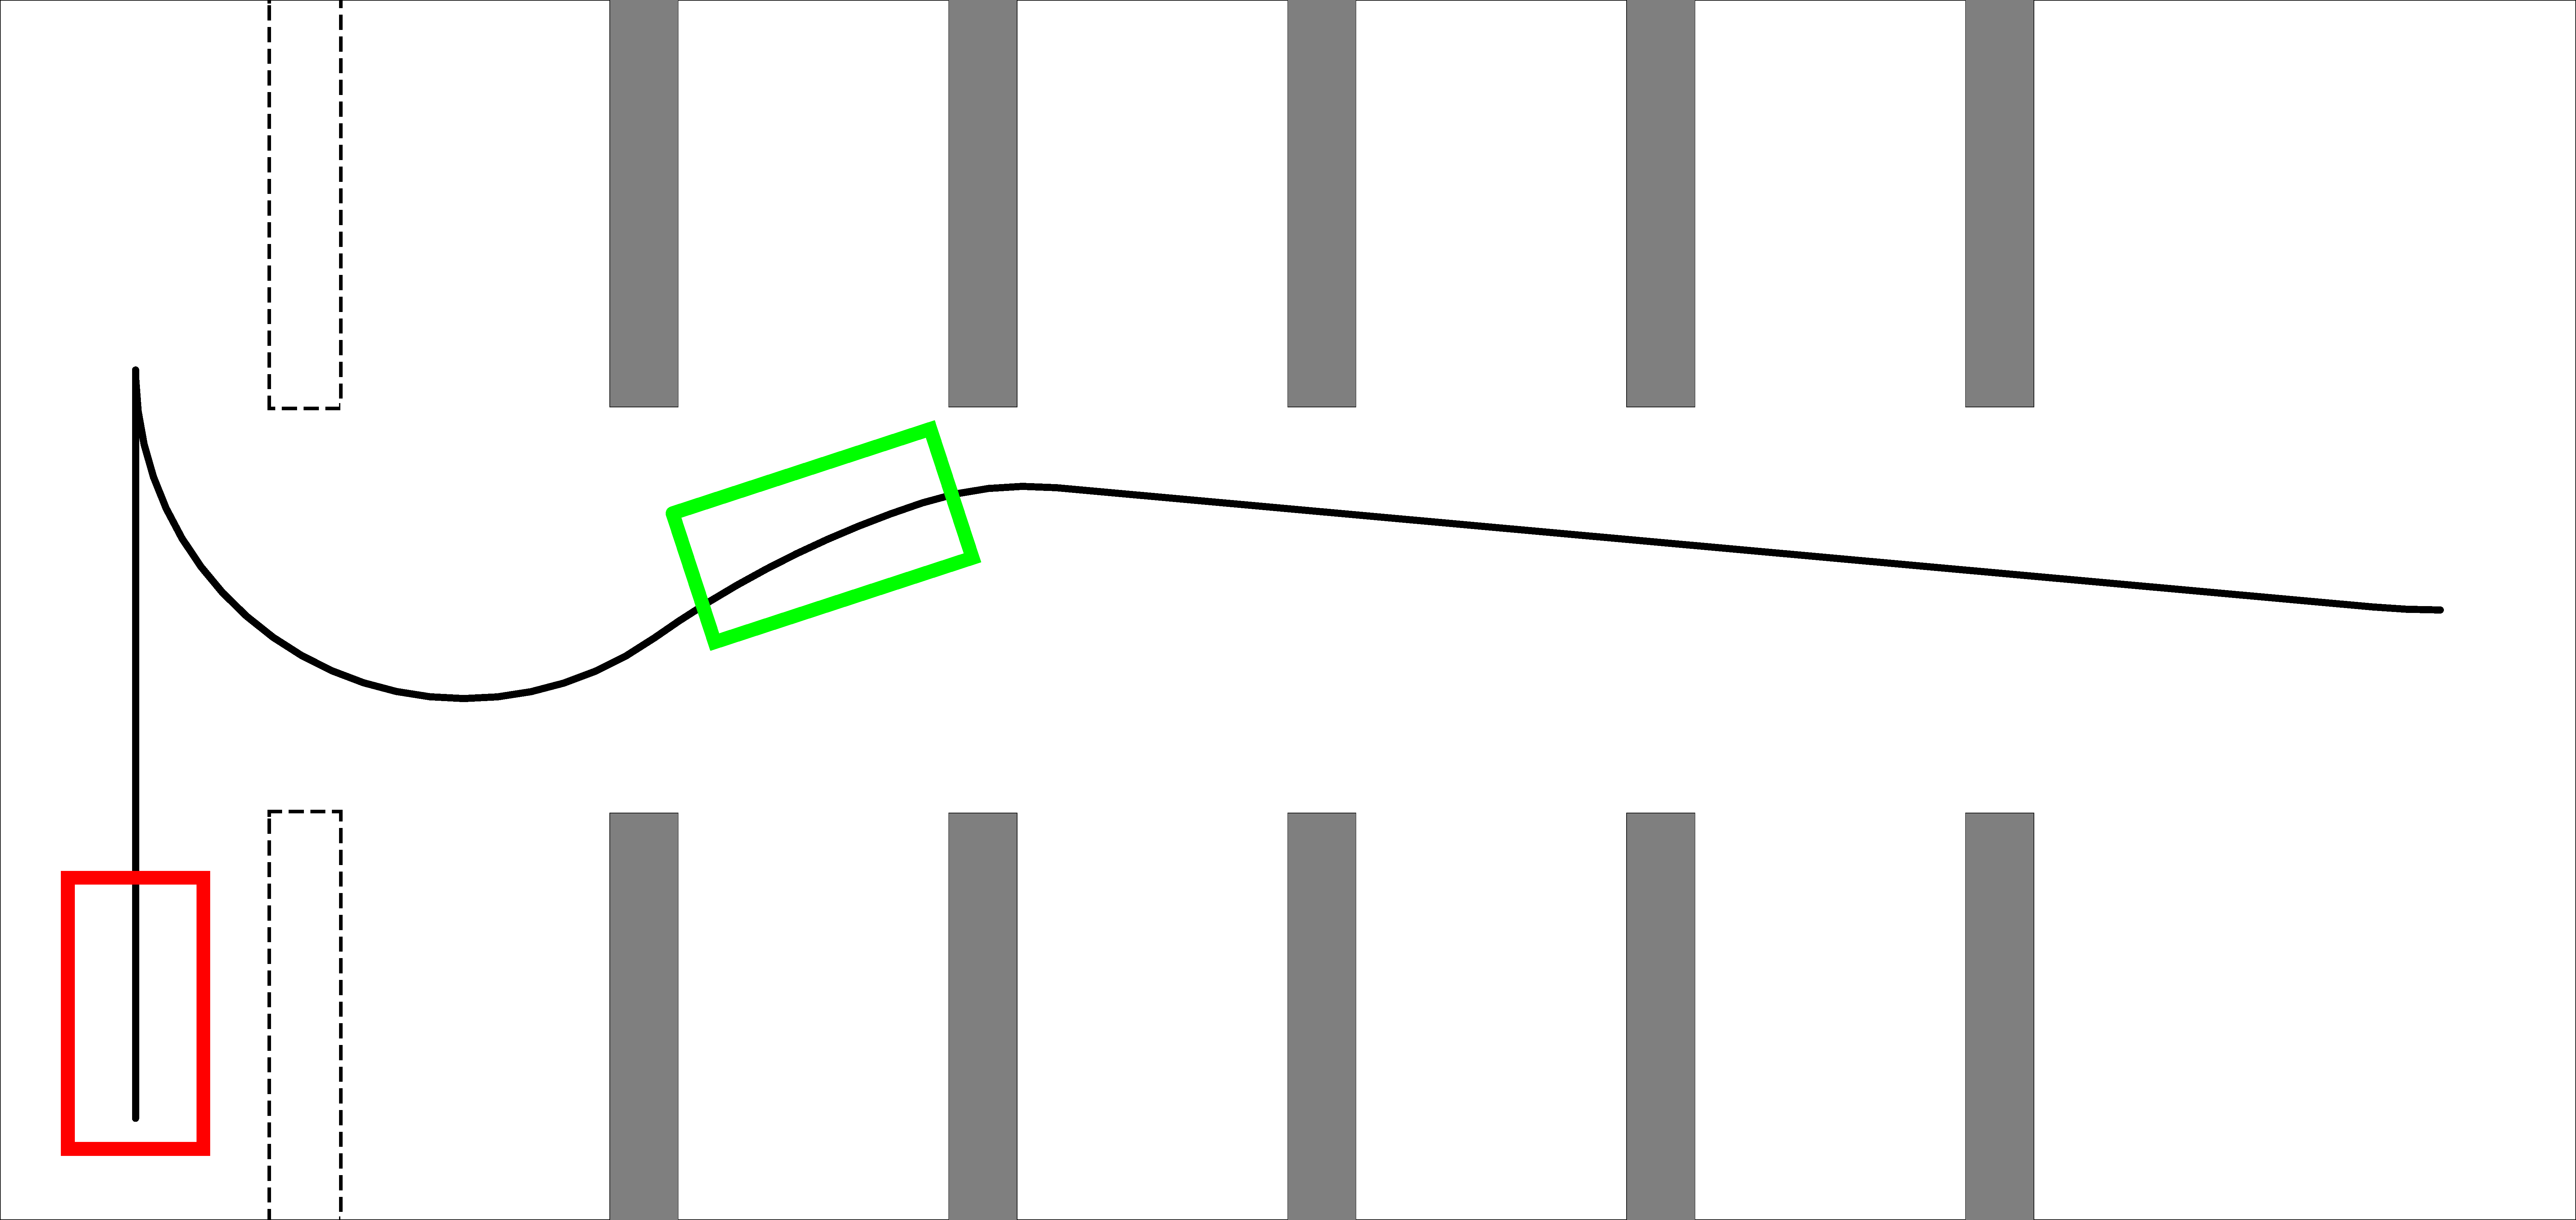
\includegraphics[height=0.35\columnwidth]{.//figures/DynamicSim/plannedPath45N.pdf}
    \label{subfig:phase4}}}        
    \caption{Five iteration of the simulation process for dynamic environment.}
    \label{fig:dynamicSim_Phases}
\end{figure}

%The algorithm of the simulation process can be seen in Algorithm~\ref{alg:dynamicSim_Alg}. The $\mathcal{E}$ indicates the structure of the environment. This structure contains the geometrical representation of the obstacles. The $\mathcal{P}_{global}$ and the  $\mathcal{P}_{approx}$  indicate the global path generated by RTR planner and the approximated path feasible for car-like robots (C*CS planner). Both path are described with a configuration list. The loop variable of the simulation is \emph{i} and we run the simulation for \emph{L} iteration.

One of the most important factors for this simulation scenario are planning time and the quality of the path. The RTR and the C*CS planners run time definitely determinate the planning time. In this Section we will focus on planning time and path quality. The quality of the path will be discussed in Section~\ref{sec:static} too. 

We compare three difference planning strategy for dynamic environment. The strategies differ in re-planning method when the path is collided:
\begin{itemize}
	\item \emph{Global Re-Planning}: The path is re-planned from the robot current configuration to the goal configuration.
	\item \emph{Local Re-Planning}: The path is re-planned from the robot current configuration to the end of the collided path segment.
	\item \emph{Global Re-Planning with Tree Reservation}: Same as the first strategy, but the goal tree in the RTR algorithm remains.
\end{itemize}

\figurename~\ref{fig:dynamicSim_Global} shows \emph{Global Re-Planning} strategy for two situation. In these figures, we marked the configuration of the robot when it detects a new obstacle, the collided path segment and the goal configuration as well. In the first scenario (see \figurename~\ref{subfig:dynamicSim_Global_Good1}, \ref{subfig:dynamicSim_Global_Good2}), the path takes from the lower, left corner to the lower, right corner. We can see, that planning to the goal configuration makes a natural path for car-like robots in this situation. However, in the next scenario (\figurename~\ref{subfig:dynamicSim_Global_Bad1}, \ref{subfig:dynamicSim_Global_Bad2}) this planning method regenerates a long path segment unnecessary. In this situation, replanning only the collided segment would cost less computing capacity and makes more simple path as well.


\begin{figure}[tb]
    \centerline{
    \subfloat[]{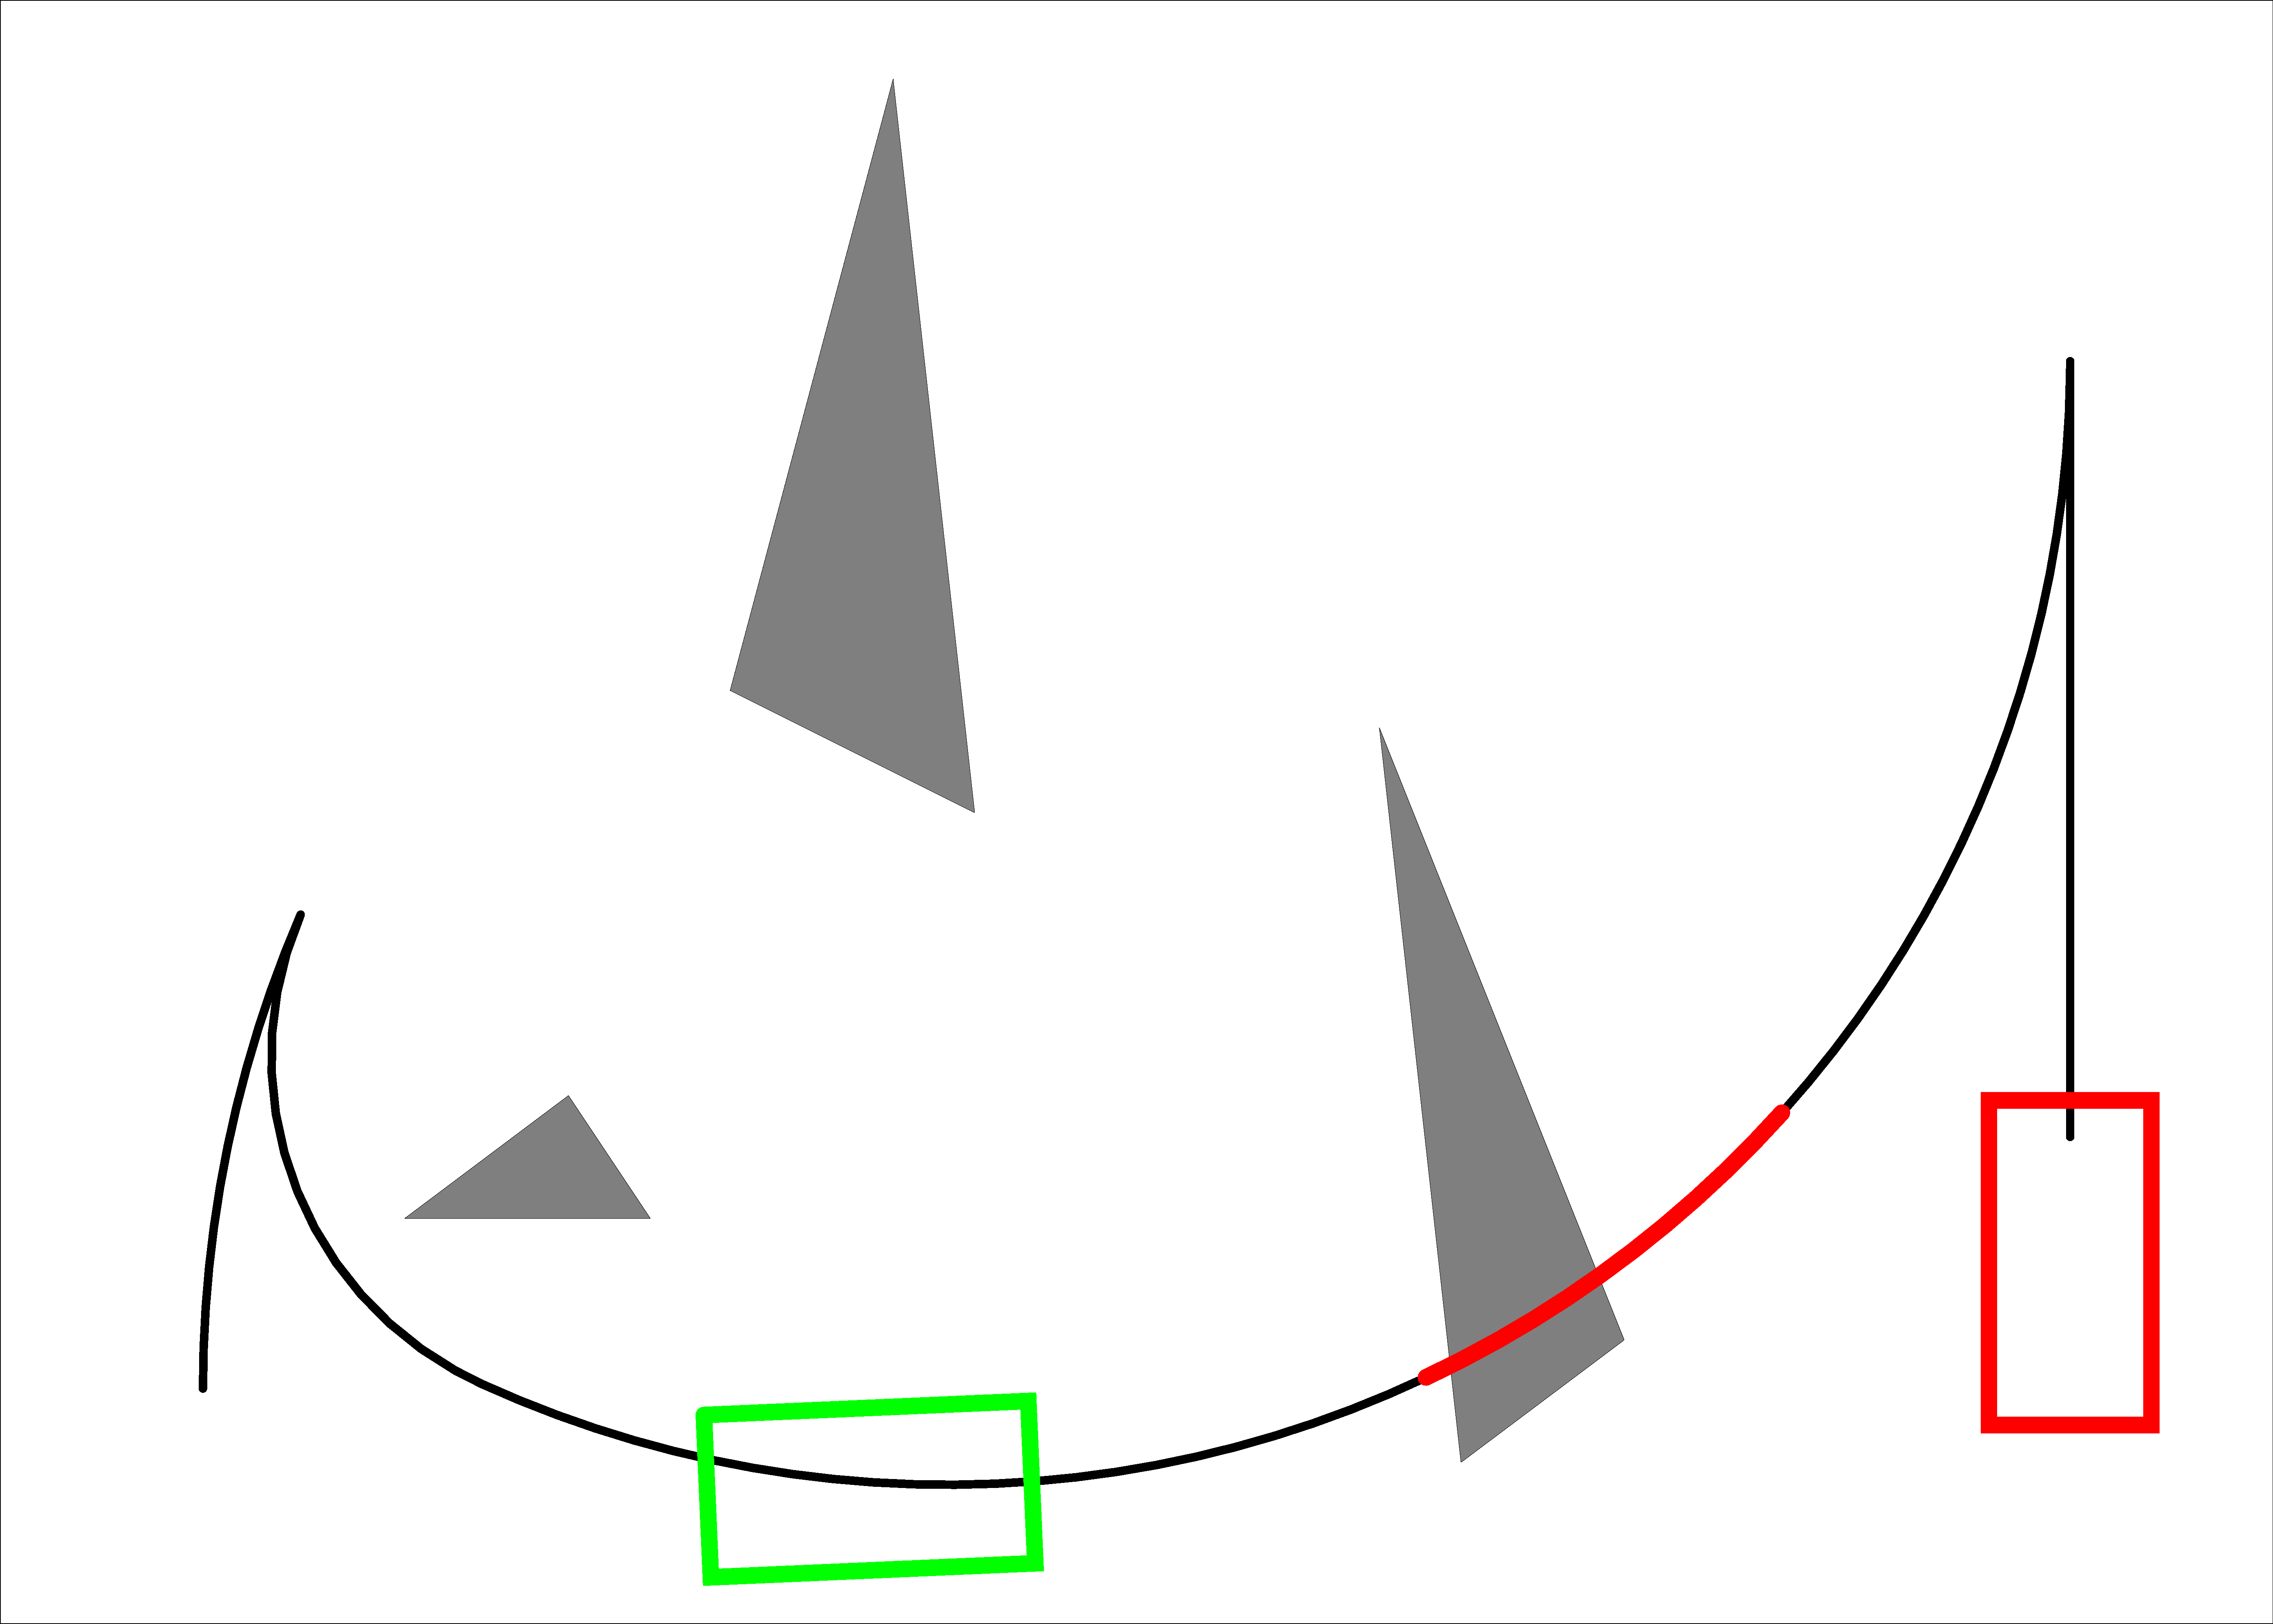
\includegraphics[height=0.35\columnwidth]{.//figures/DynamicSim/Global/plannedPath40C.pdf}
    \label{subfig:dynamicSim_Global_Good1}}
    \hfil
    \subfloat[]{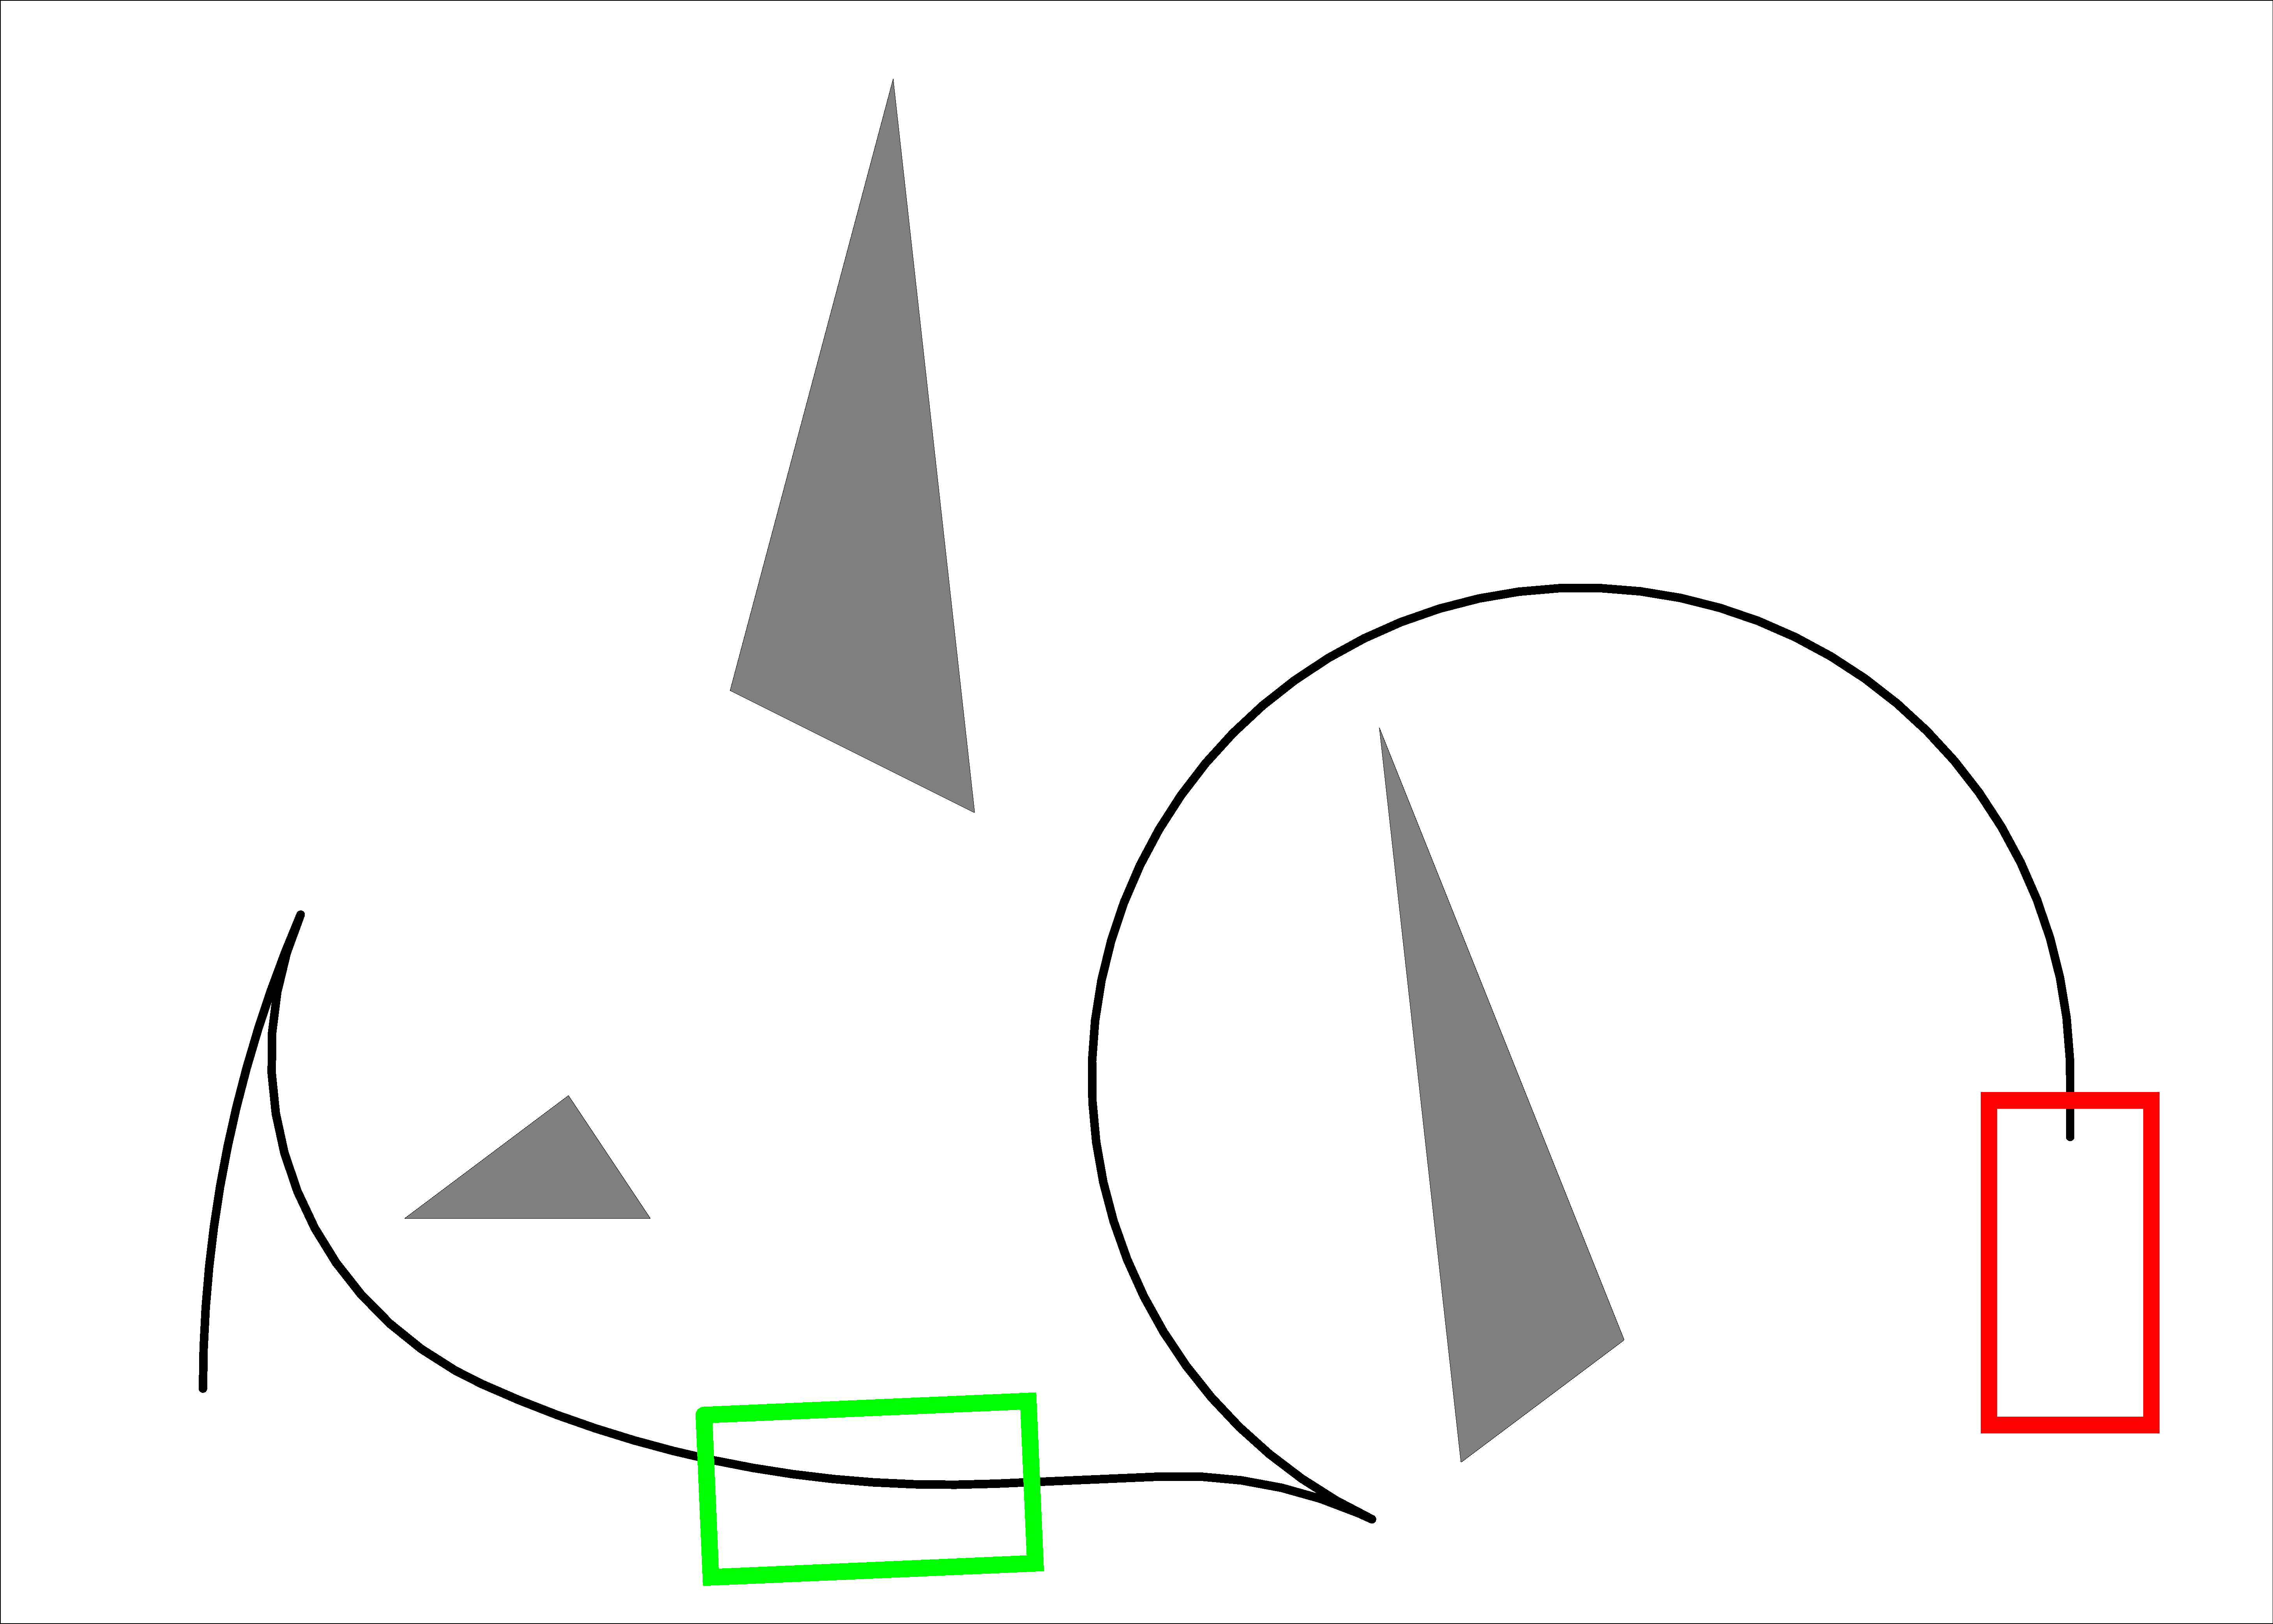
\includegraphics[height=0.35\columnwidth]{.//figures/DynamicSim/Global/plannedPath40N.pdf}
    \label{subfig:dynamicSim_Global_Good2}}
    }
    \centerline{
    \subfloat[]{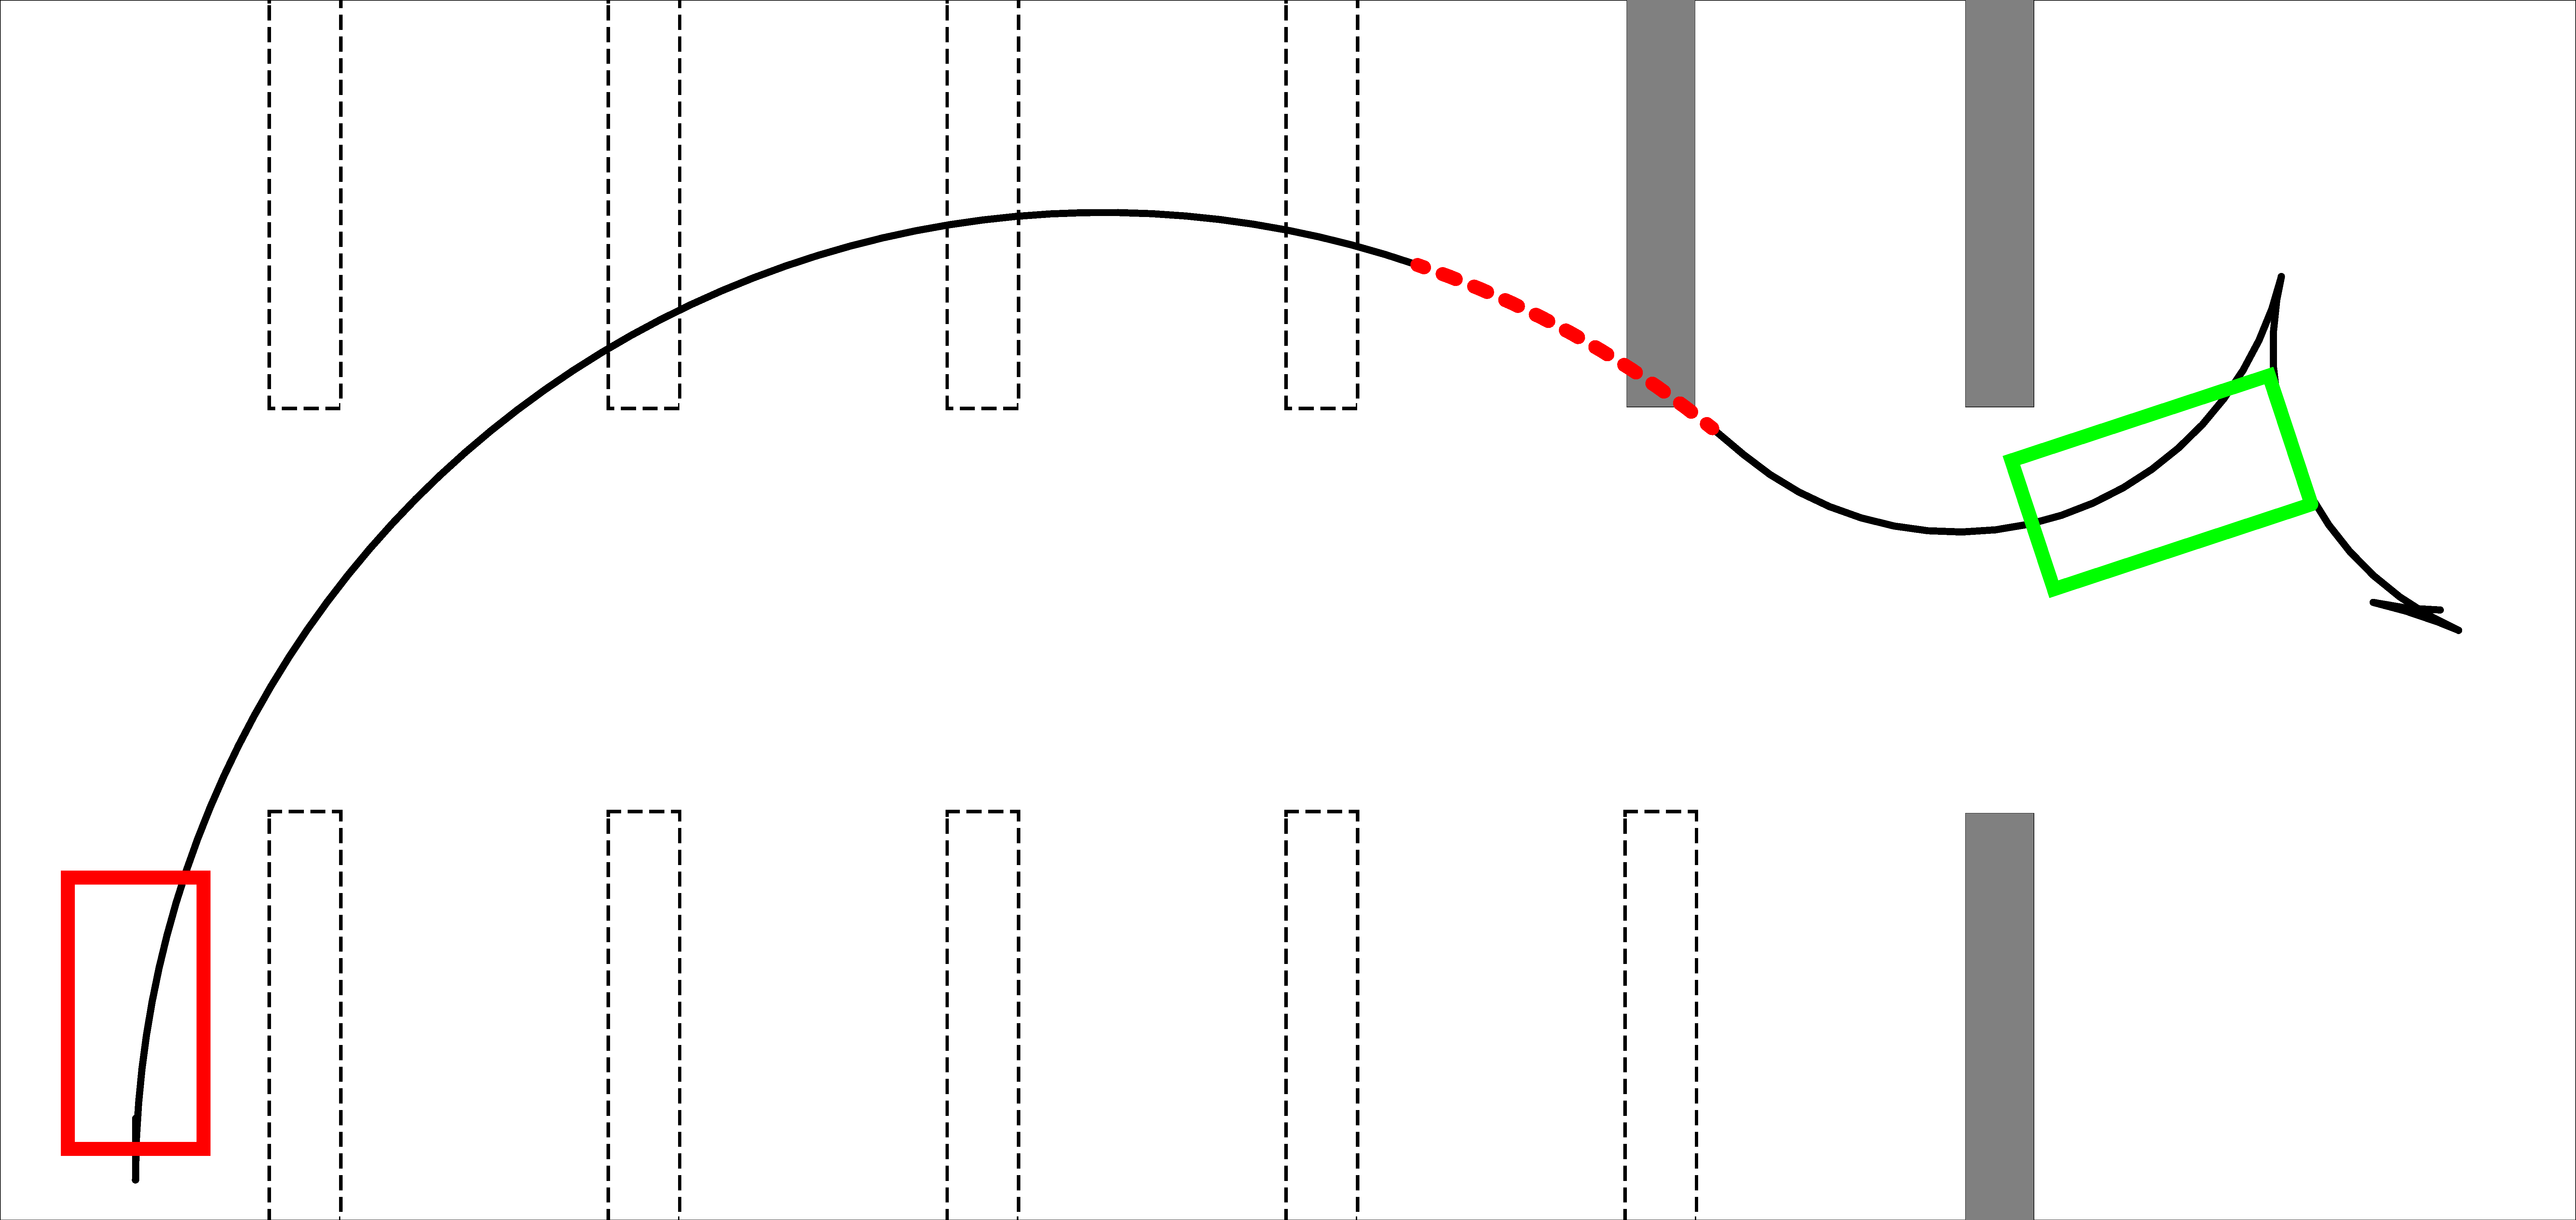
\includegraphics[height=0.45\columnwidth]{.//figures/DynamicSim/Global/plannedPath30C.pdf}
    \label{subfig:dynamicSim_Global_Bad1}}
    }
    \centerline{    
    \subfloat[]{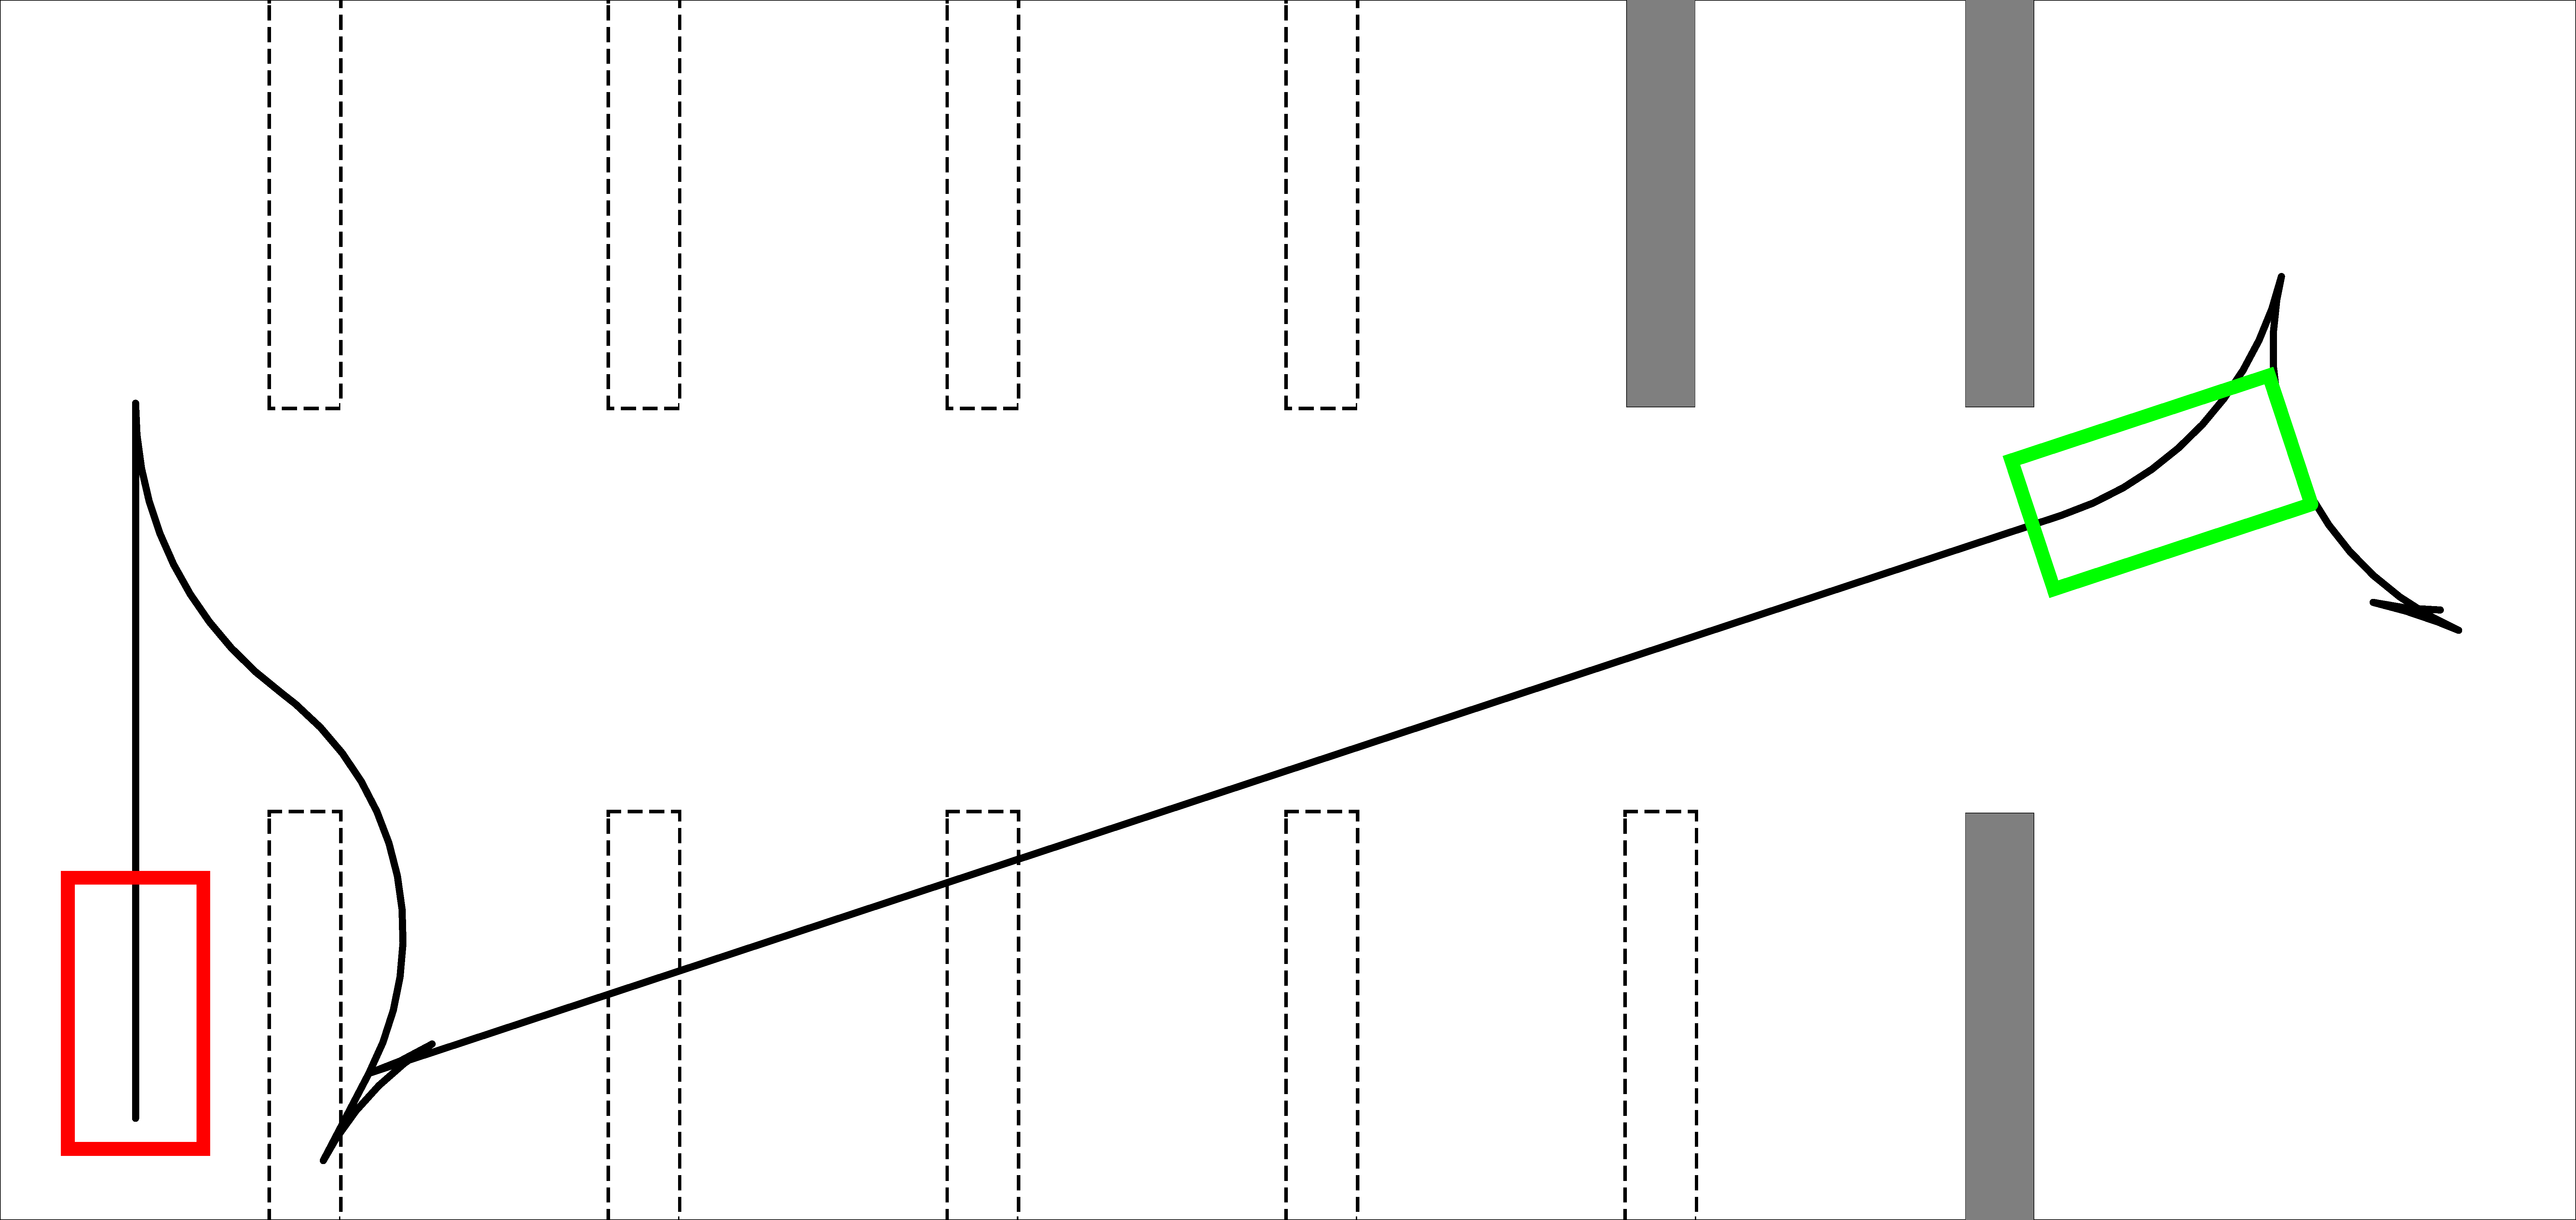
\includegraphics[height=0.45\columnwidth]{.//figures/DynamicSim/Global/plannedPath30N.pdf}
    \label{subfig:dynamicSim_Global_Bad2}}
    }
    \caption{Scenes for \emph{Global Re-Planning} strategy. (a,c) Before re-plan, (b,d) After re-plan.}
    \label{fig:dynamicSim_Global}
\end{figure}

\begin{figure}[tb]
    \centerline{
    \subfloat[]{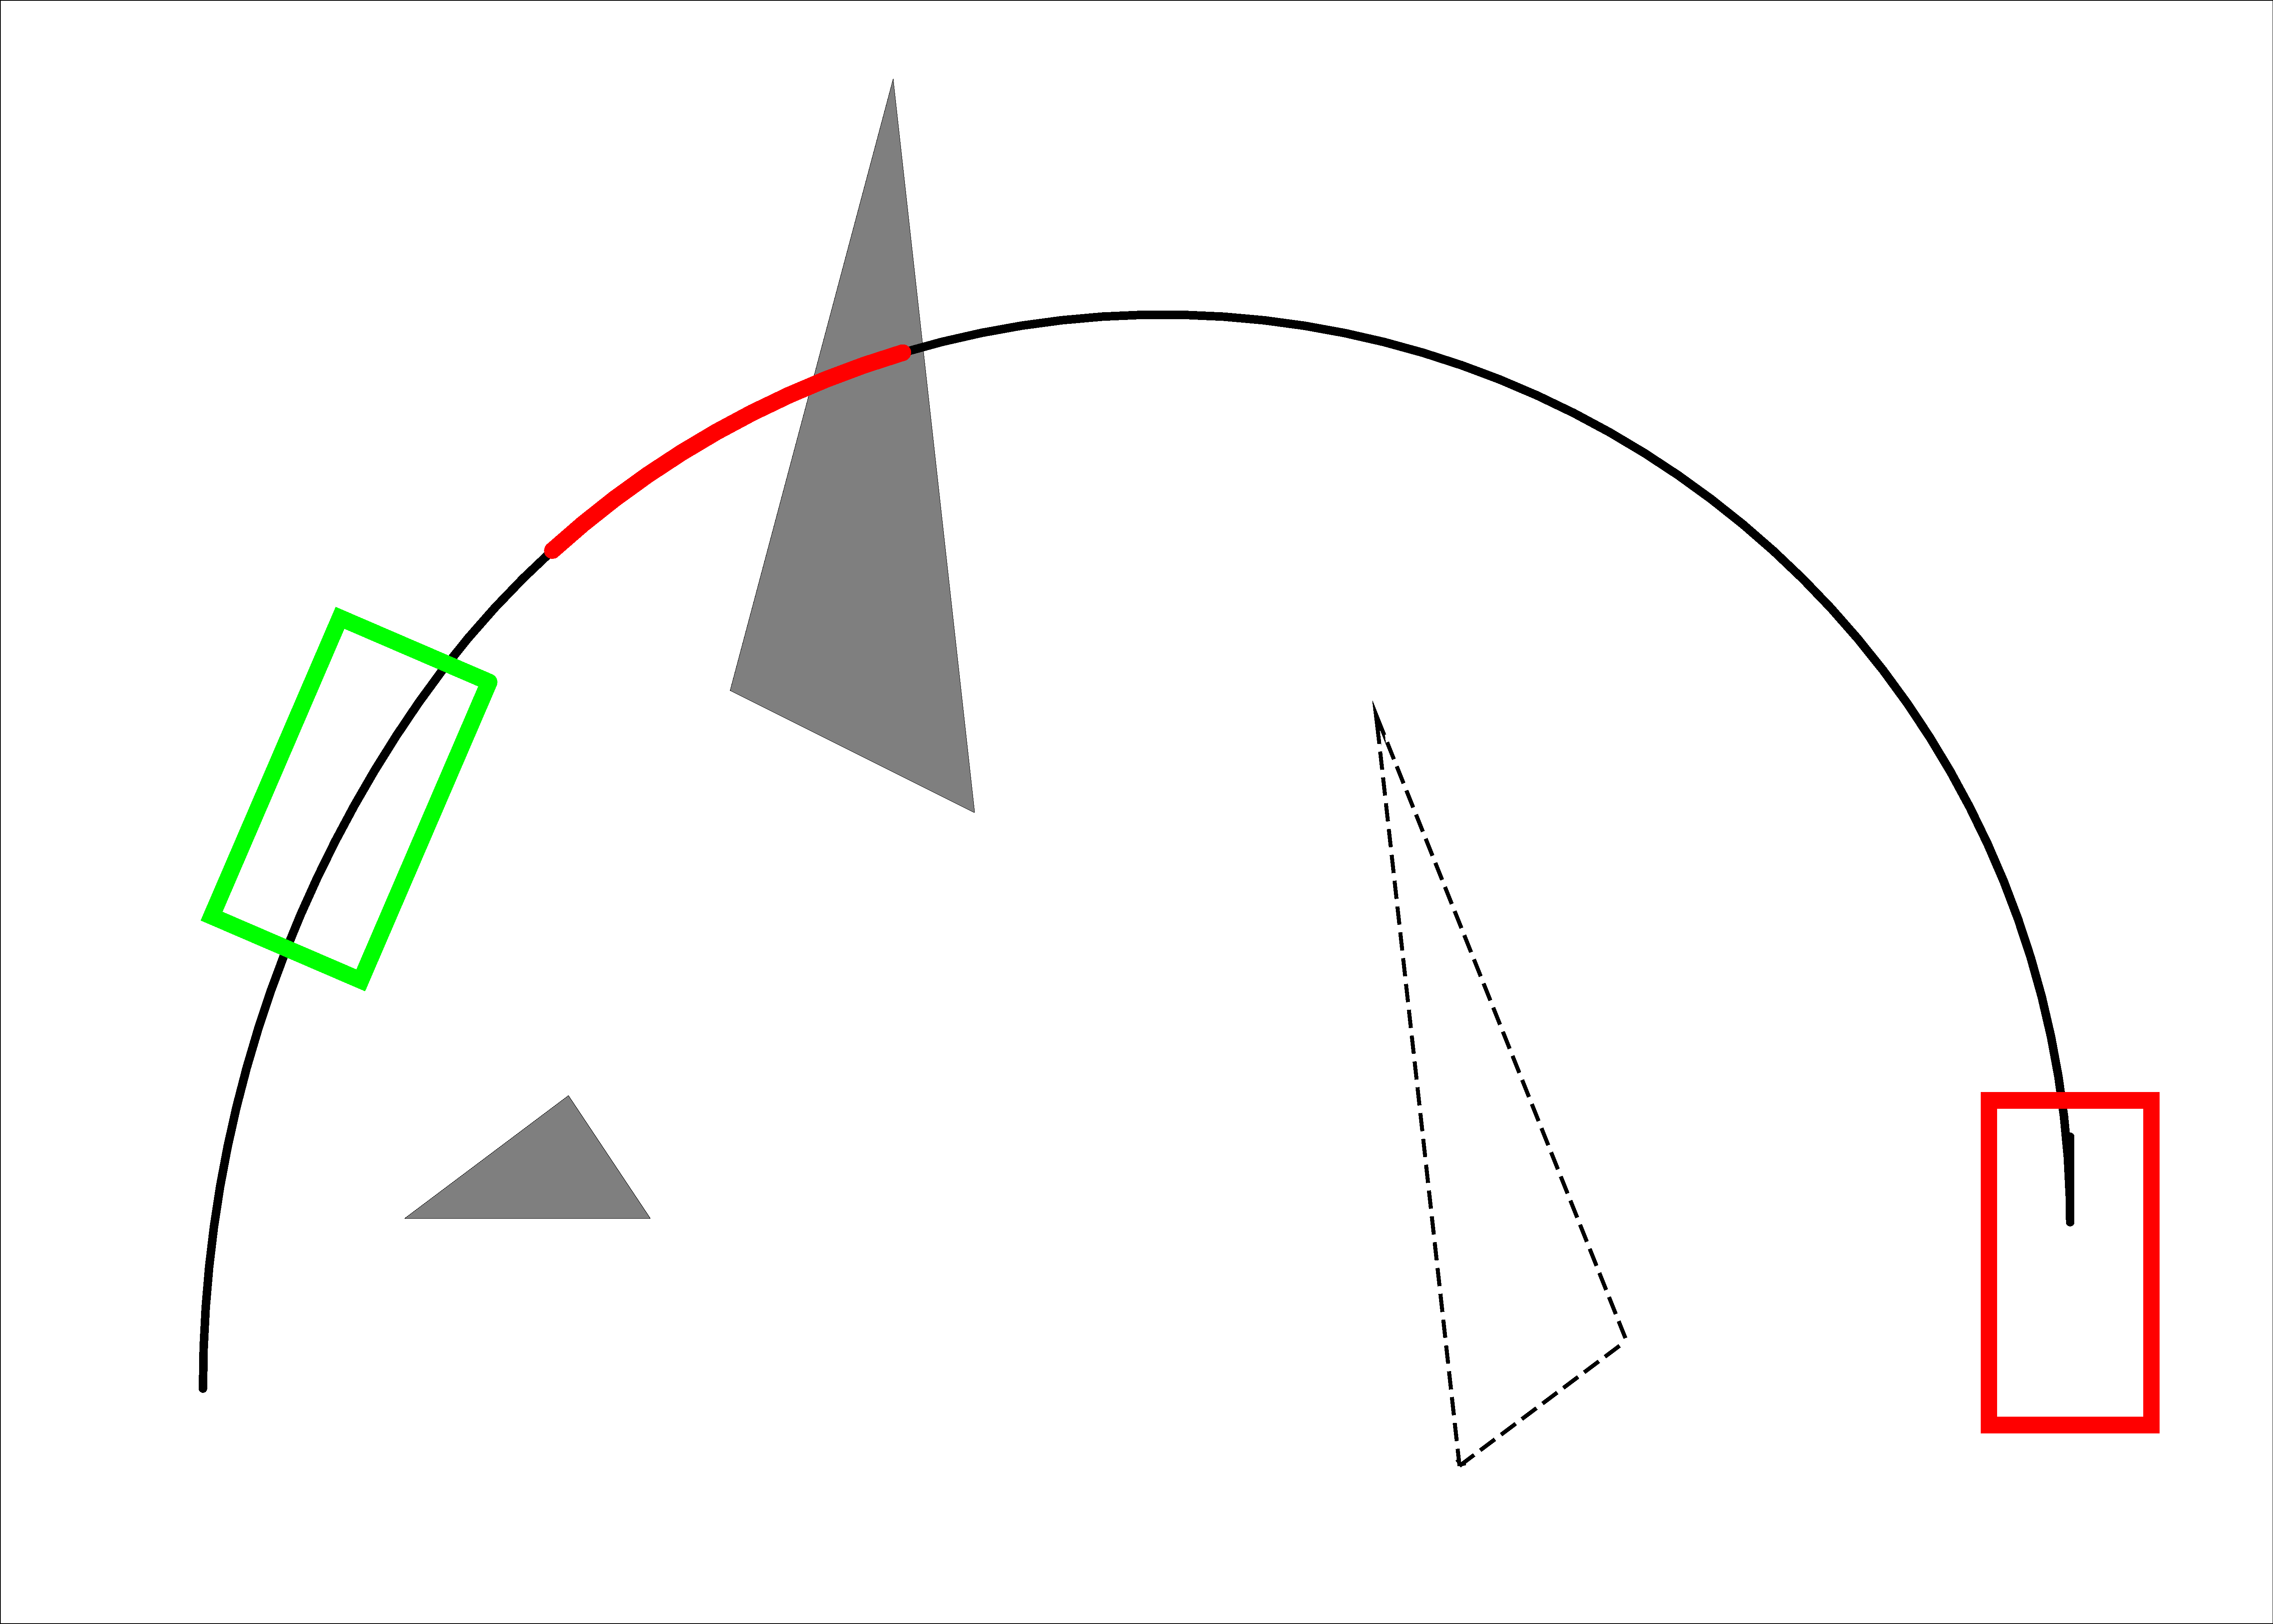
\includegraphics[height=0.35\columnwidth]{.//figures/DynamicSim/Local/plannedPath12C.pdf}
    \label{subfig:dynamicSim_Local_Bad1}}
    \hfil
    \subfloat[]{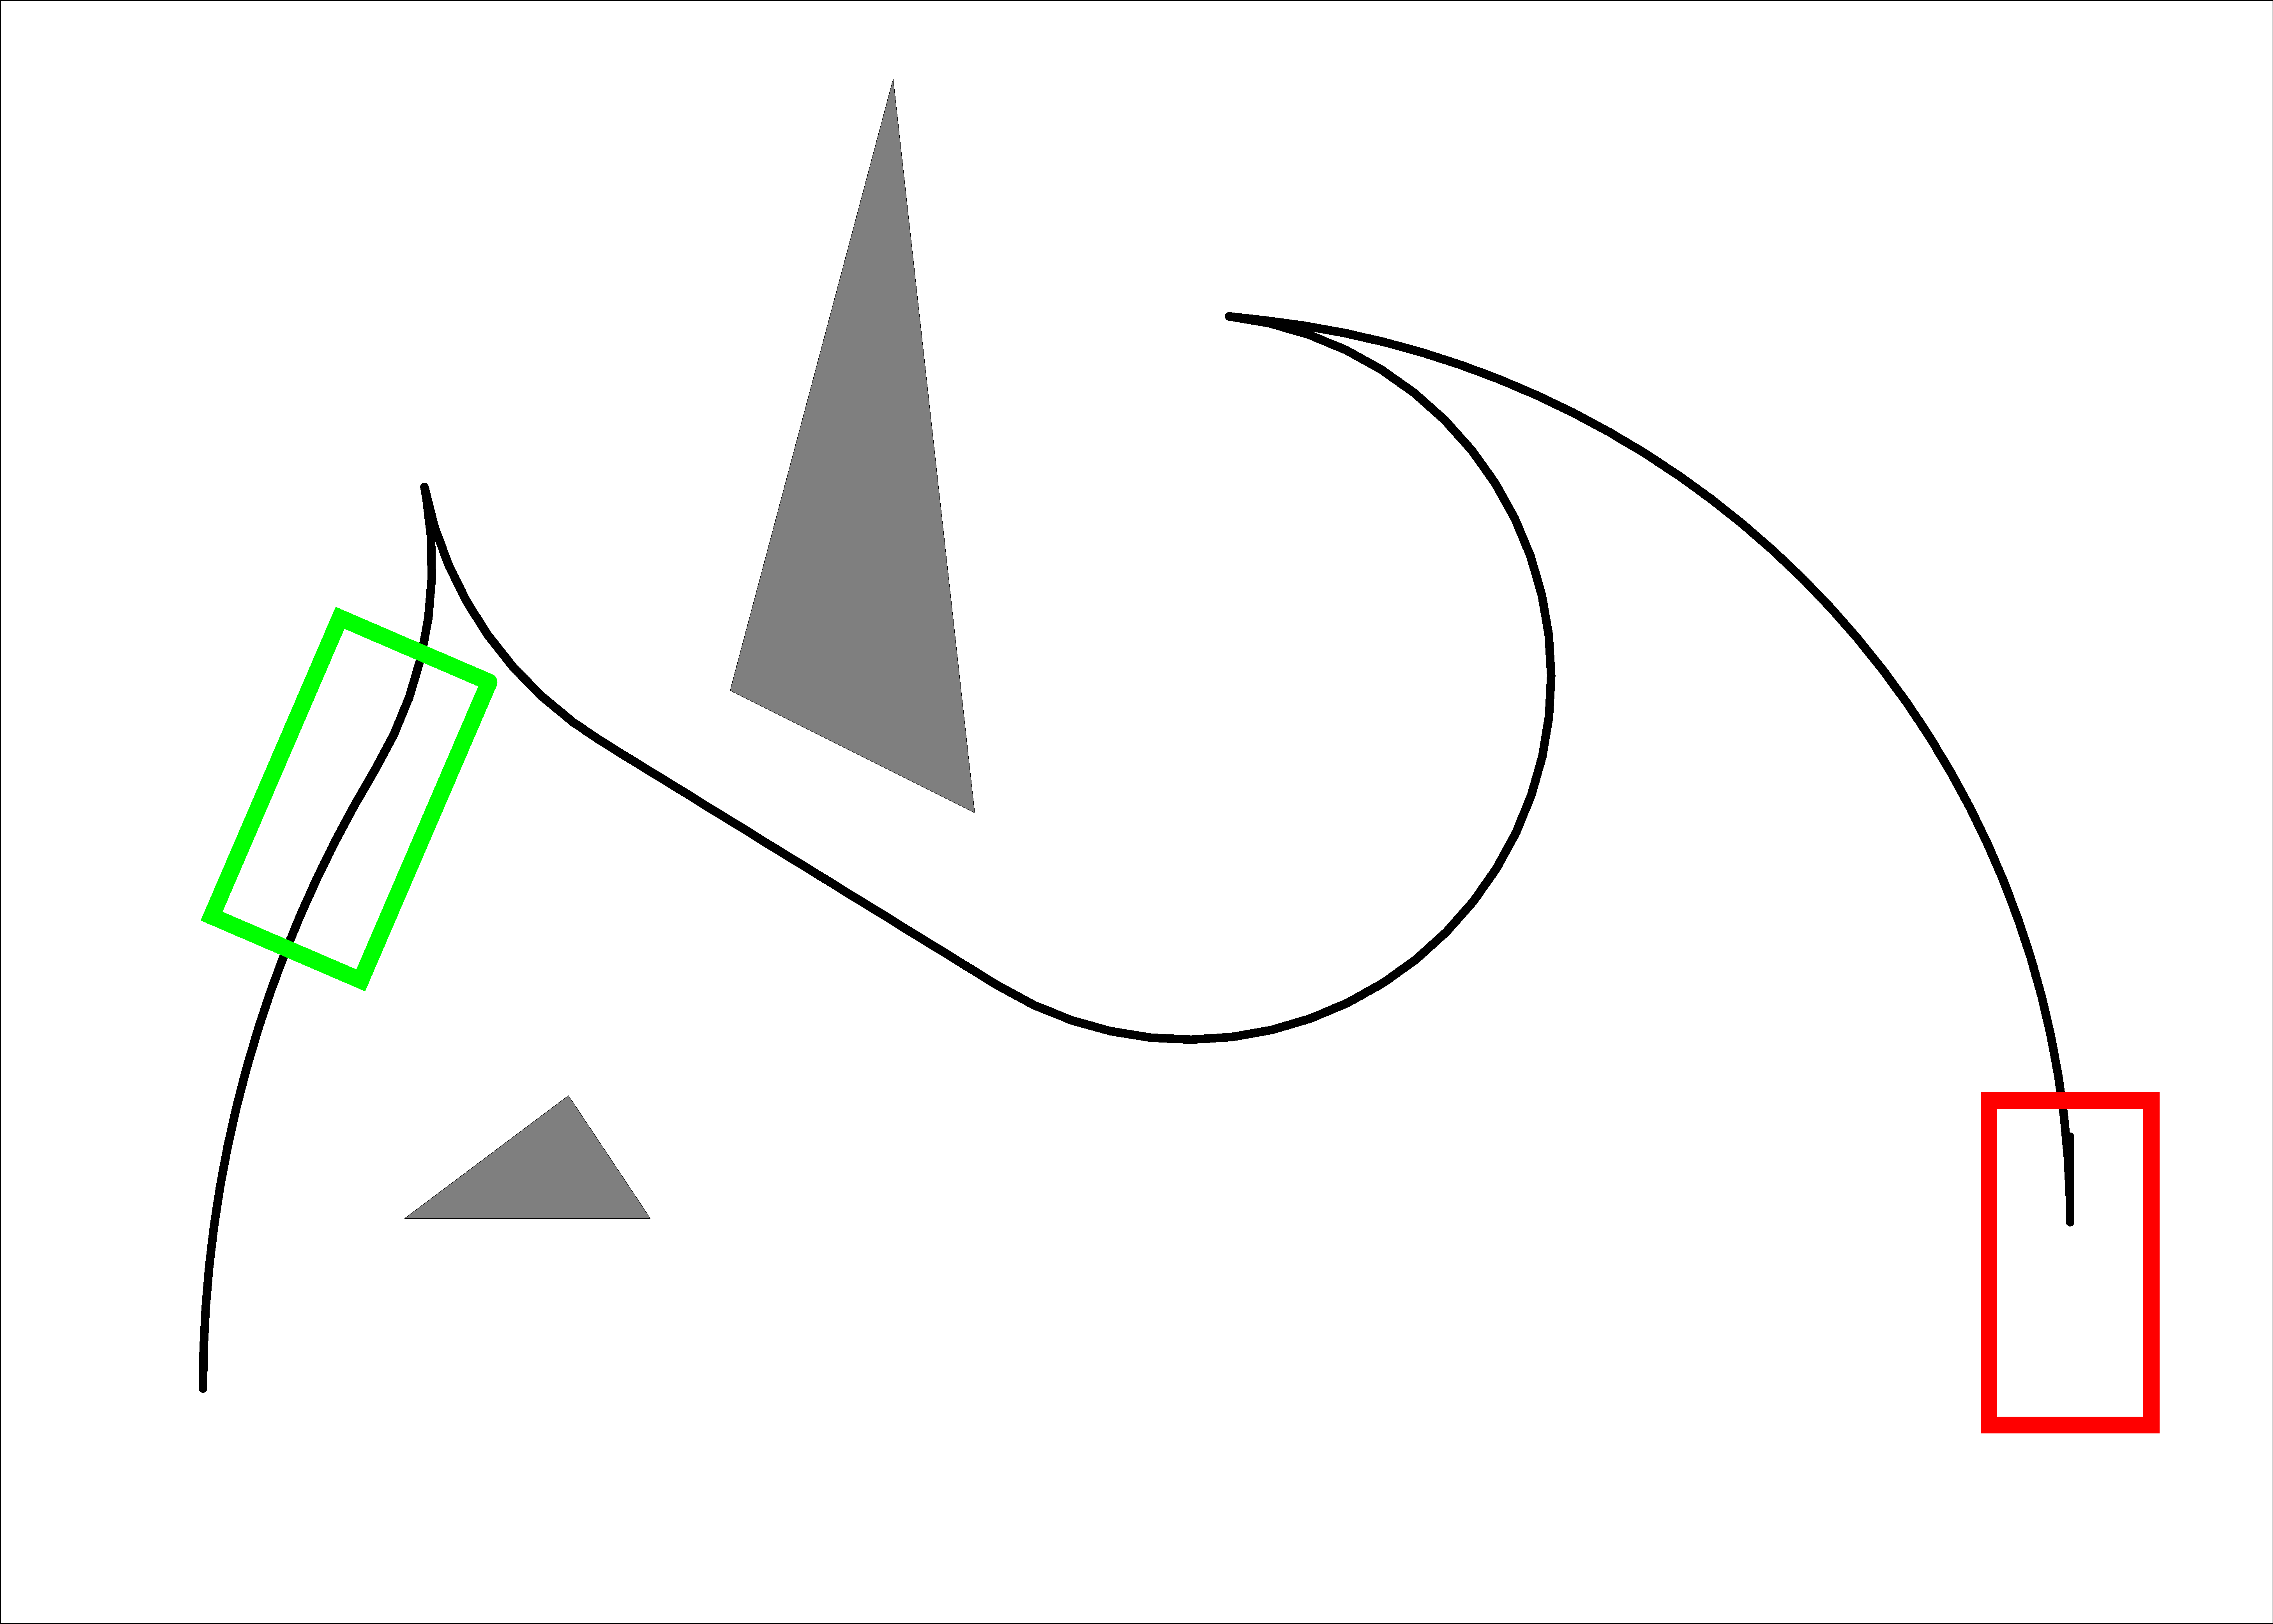
\includegraphics[height=0.35\columnwidth]{.//figures/DynamicSim/Local/plannedPath12N.pdf}
    \label{subfig:dynamicSim_Local_Bad2}}
    }
    \centerline{
    \subfloat[]{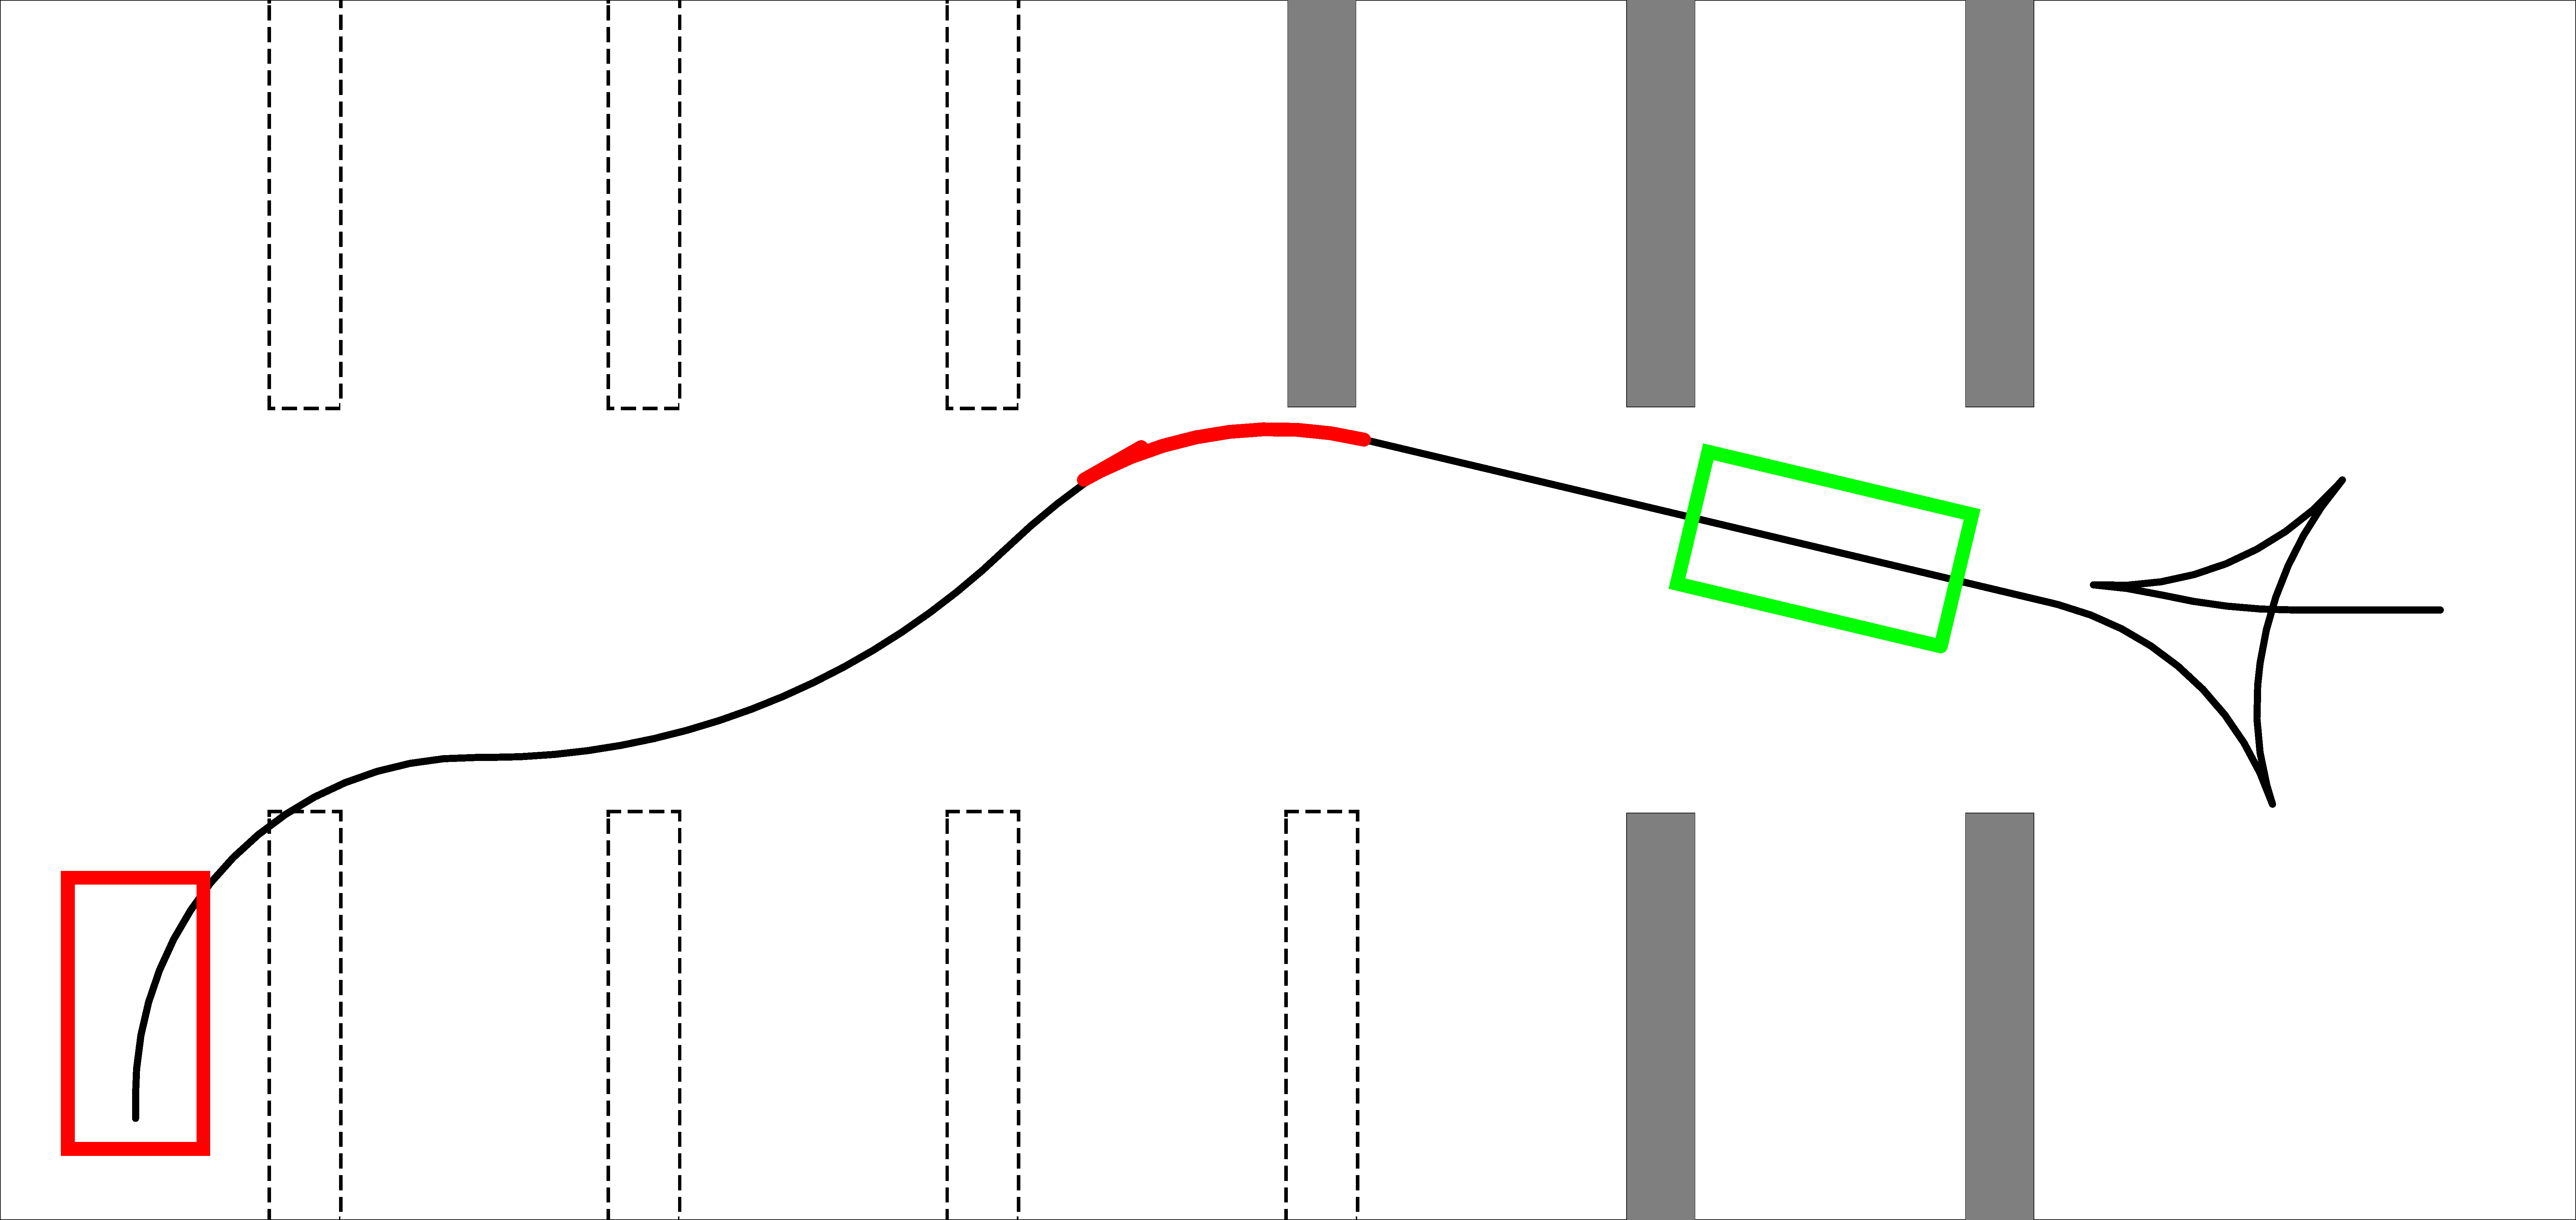
\includegraphics[height=0.45\columnwidth]{.//figures/DynamicSim/Local/plannedPath56C.pdf}
    \label{subfig:dynamicSim_Local_Good1}}
    }
    \centerline{    
    \subfloat[]{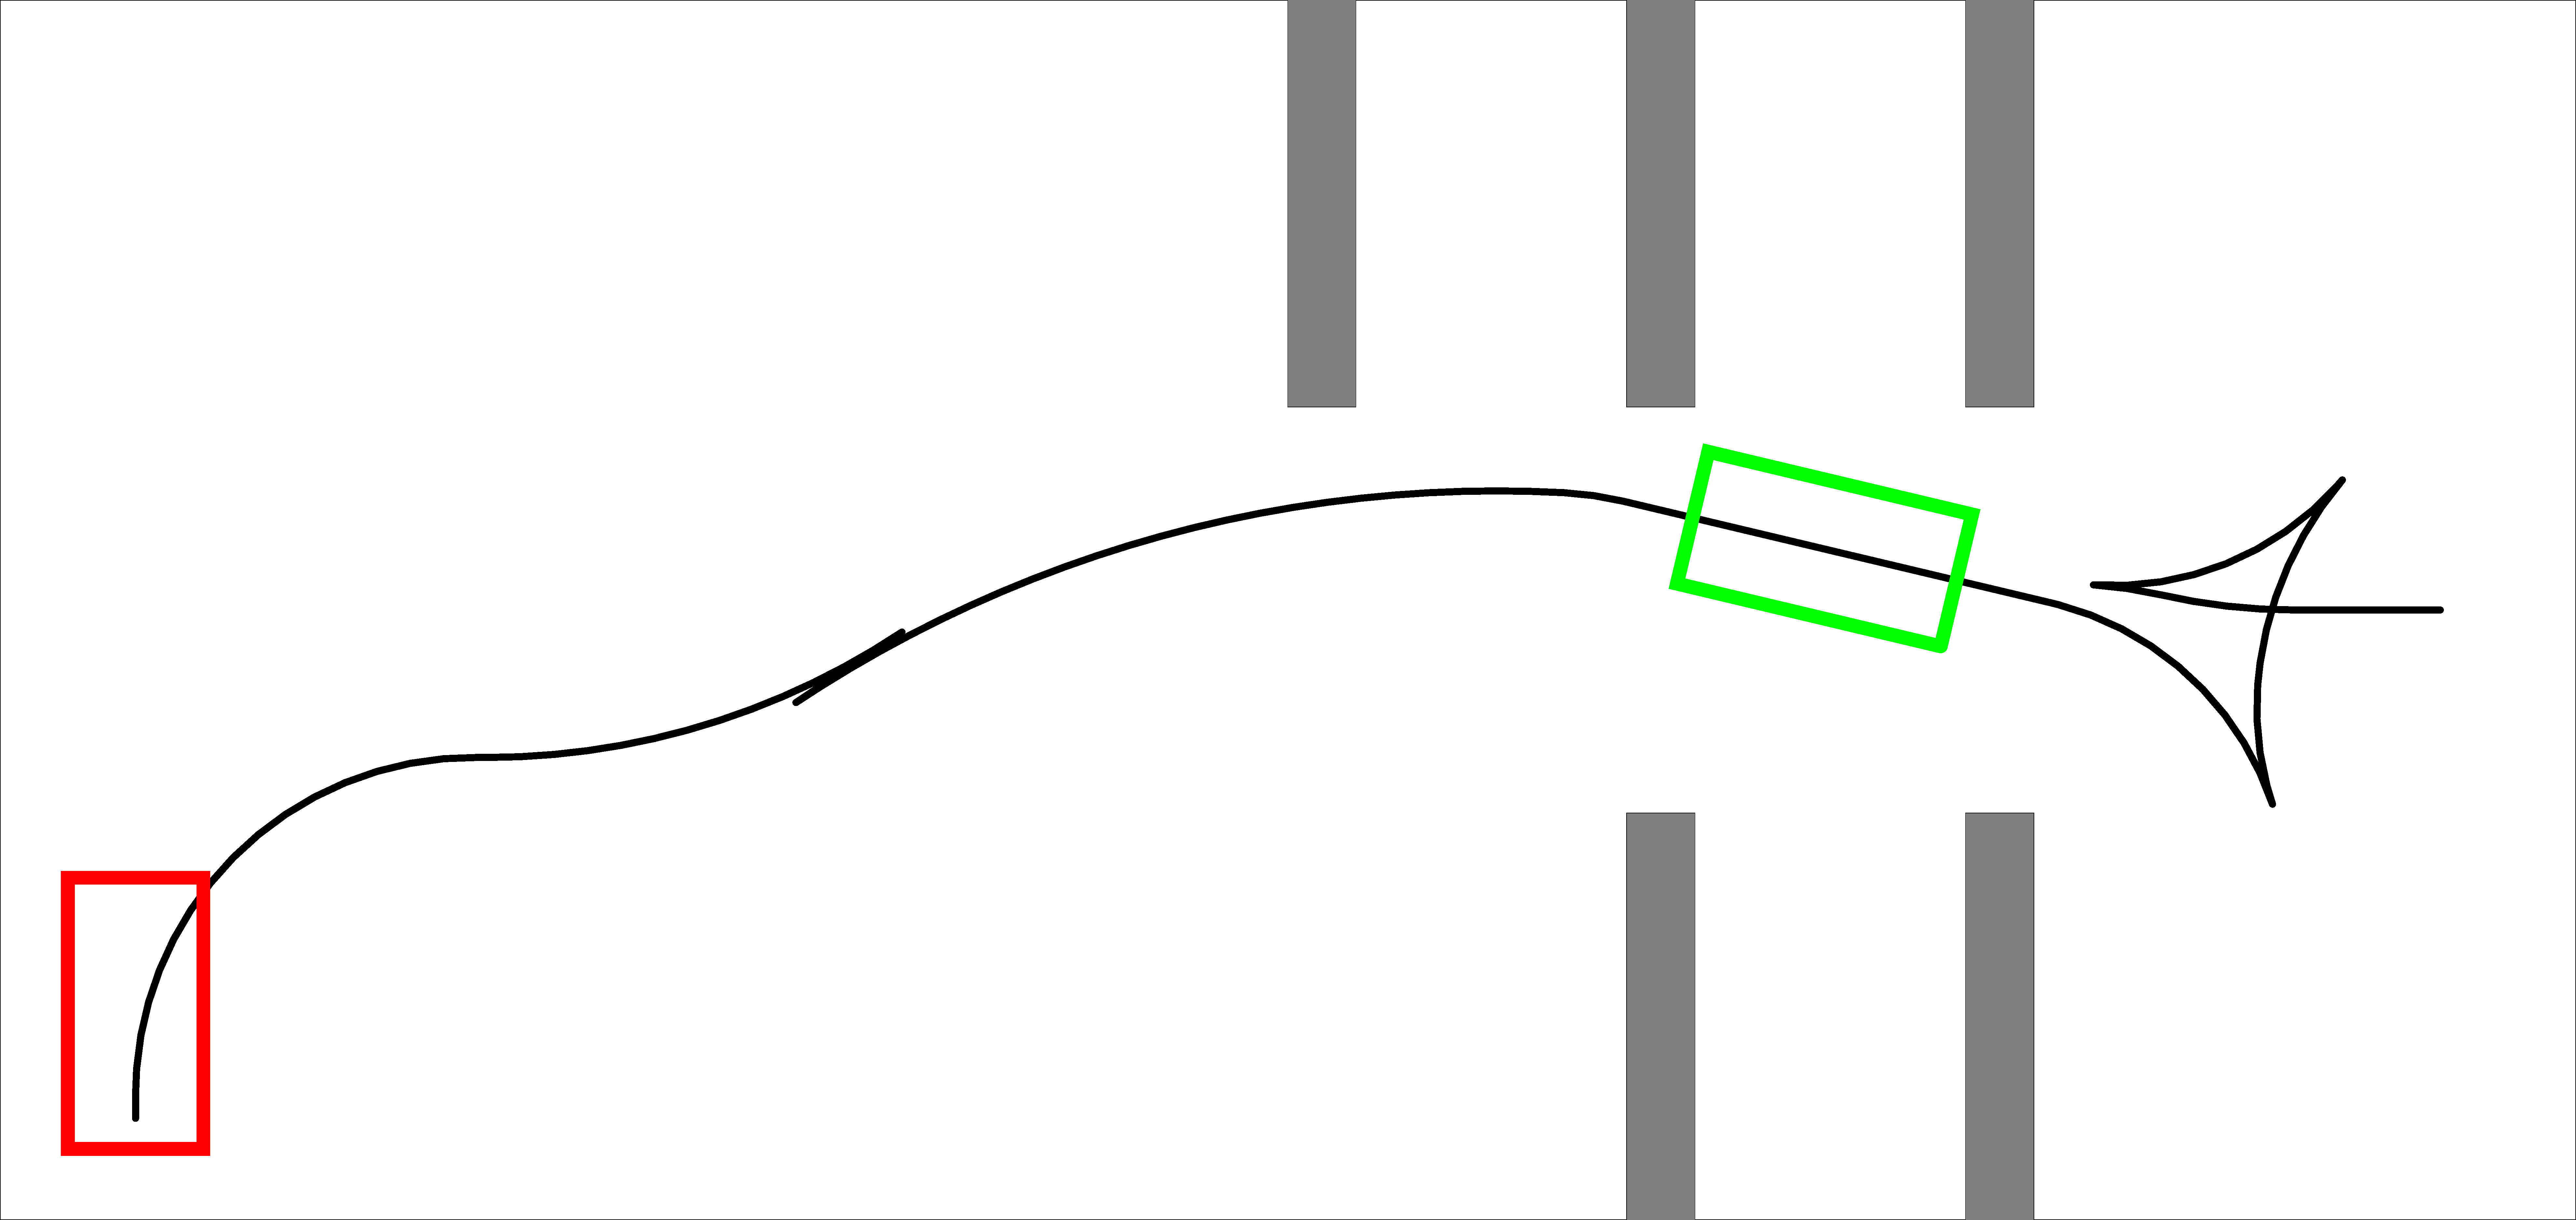
\includegraphics[height=0.45\columnwidth]{.//figures/DynamicSim/Local/plannedPath56N.pdf}
    \label{subfig:dynamicSim_Local_Good2}}
    }
    \caption{Scenes for \emph{Local Re-Planning} strategy. (a,c) Before re-plan, (b,d) After re-plan.}
    \label{fig:dynamicSim_Local}
\end{figure}

The \emph{Local Re-Planning} strategy is shown in \figurename~\ref{fig:dynamicSim_Local}. In the first situation (\figurename~\ref{subfig:dynamicSim_Local_Bad1}, \ref{subfig:dynamicSim_Local_Bad2}), this method generates complicated path, because the planner tries to connect the new path segment to existing one. In this strategy, there is an extra parameter, which determinate the distance from the end point of the collided segment to the end point of the generated segment. If this parameter set to infinity, the strategy will be \emph{Global Re-Planning} method. In the second scene (\figurename~\ref{subfig:dynamicSim_Local_Good1}, \ref{subfig:dynamicSim_Local_Good2}), the local planning makes a simple, natural solution and do not re-plan unnecessary.

The \emph{Global Re-Planning with Tree Reservation} method generates path to the goal configuration like the \emph{Global Re-Planning} algorithm. The tree reservation is an improvement in the RTR algorithm. After the first run of the global planner, the RTR does not rebuild the entire \emph{goal tree}, instead it uses the tree built in the first iteration. As a disadvantage of this improvement, the planner has to remove the collided nodes and edges from the \emph{goal tree} and it takes time to check the whole tree.

In \tablename~\ref{table:dynamicSim_RunTimes} we compare the three different planning strategies run time. We have run twenty measurement for every scene with every strategy, and averaged the results. The algorithms were implemented in C++ and tested on a notebook computer with Intel i7-3630QM processor running at $2.4GHz$ and having 8 GB RAM.

In the first scene the \emph{Local Re-Planning} strategy gives better run time, but in the second scene \emph{Global Re-Planning} has lower run time. We see the same result with path quality, so local or global re-planning strongly depends on the environment. The global strategy with tree reservation has lower run time for the first two scene. So in most case the extra collision check in this method cause small run time growth.

\begin{table}[t]
\renewcommand{\arraystretch}{1.3}
\caption{Run Times for Different Planning Strategies}
\label{table:dynamicSim_RunTimes}
\centering
\begin{tabular}{l*{6}{c}r}
\bfseries Scene & \bfseries Global Re-Pl. & \bfseries Local Re-Pl. & \bfseries Global Re-Pl. with T. R. \\
\hline
\emph{Scene 1}			& 64.9375ms		& 56.1083ms		& 44.375ms\\
\emph{Scene 2}    		& 7.2250ms		& 7.625ms		& 6.425ms\\
\emph{Scene 3}    		& 8.40875ms		& 8.27795ms		& 12.3391ms\\
\end{tabular}
\end{table}

%\begin{algorithm}[tb]
%	\begin{algorithmic}[1]
%		\State $\operatorname{\mathcal{P}_{global}} \gets \operatorname{GLOBAL\_PLANNER}(\mathcal{E})$
%		\State $\operatorname{\mathcal{P}_{approx}} \gets \operatorname{LOCAL\_PLANNER}(\mathcal{E}, \mathcal{P})$
%		\ForAll{ $i = 1$ to $L$}
%			\If {$\operatorname{CHECK\_OBSTACLES}(\mathcal{E})$}
%				\If {$\operatorname{CHECK\_COLLISION}(\mathcal{E}, \mathcal{P})$}
%					\State $\operatorname{\mathcal{P}_{global}} \gets \operatorname{GLOBAL\_PLANNER}(\mathcal{E})$
%					\State $\operatorname{\mathcal{P}_{approx}} \gets \operatorname{LOCAL\_PLANNER}(\mathcal{E}, \mathcal{P})$
%				\EndIf
%			\EndIf
%		\EndFor
%	\end{algorithmic}
%	\caption{The simulation method for planning in dynamic environment}
%	\label{alg:dynamicSim_Alg}
%\end{algorithm}

\begin{figure}[tb]
    \centerline{
    \subfloat[]{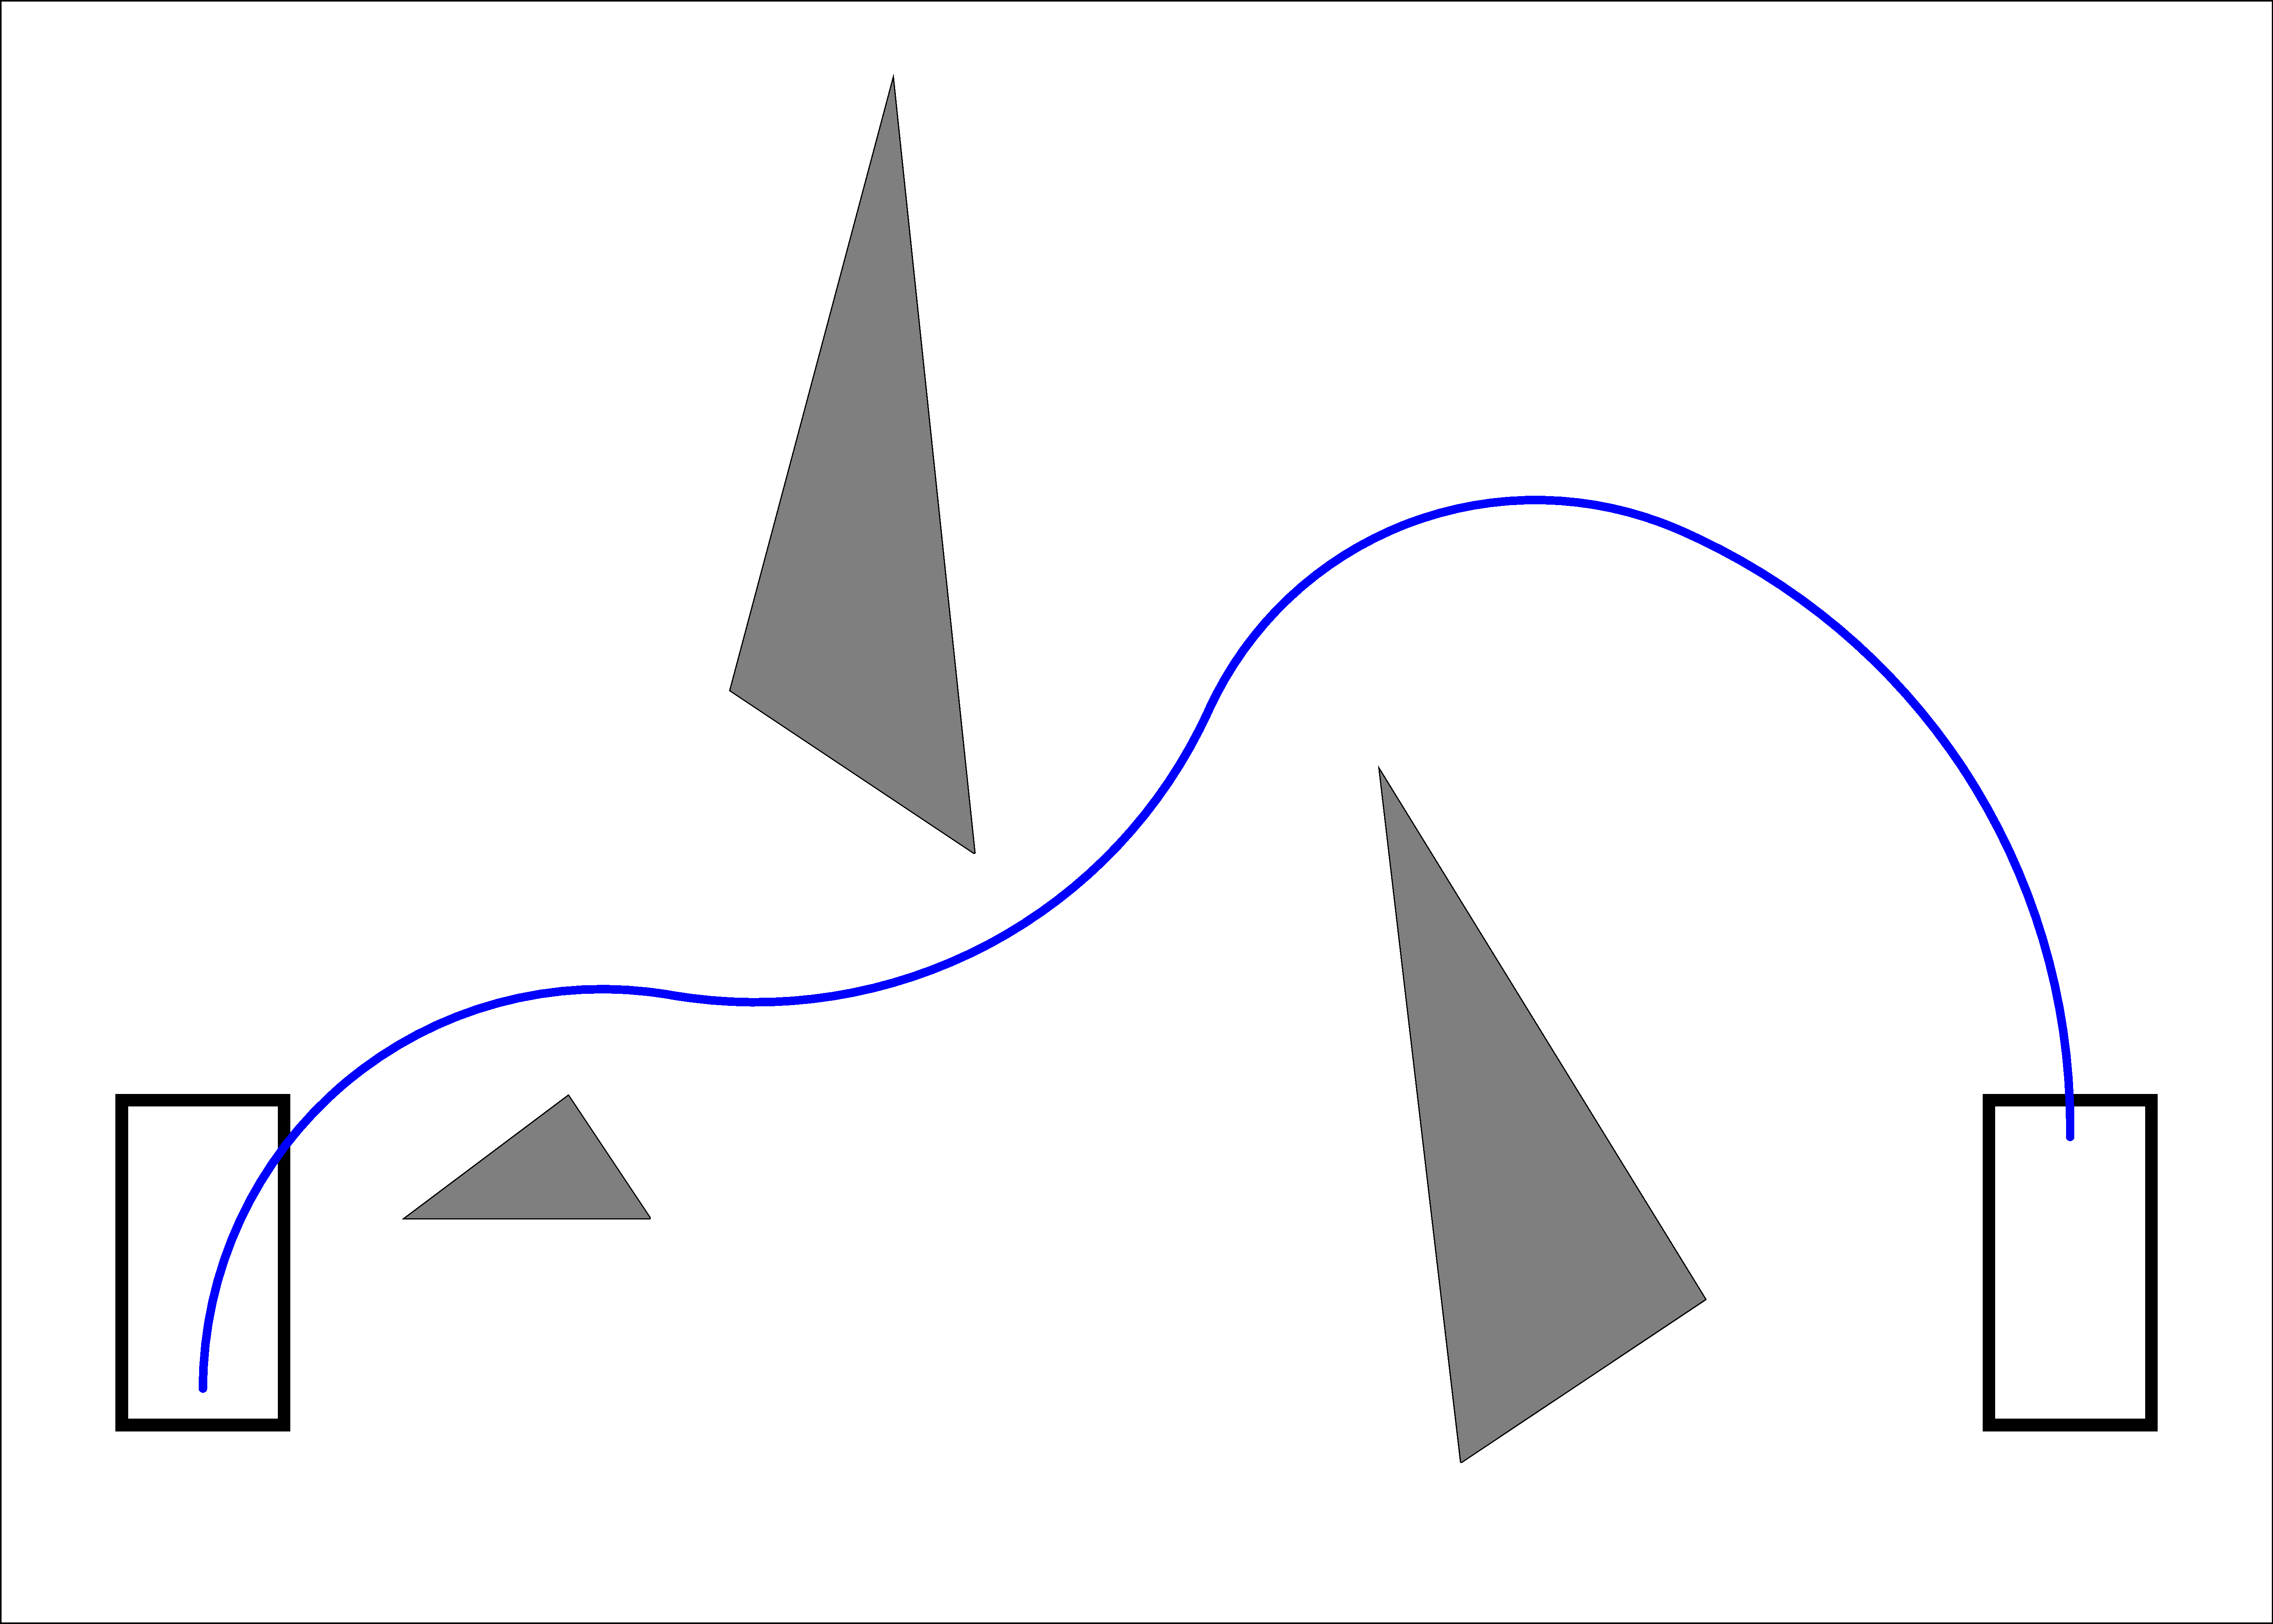
\includegraphics[width=0.49\columnwidth]{.//figures/StaticSim/frameFreeCusps.pdf}
    \label{subfig:frameFreeCusps}}
    \hfil
    \subfloat[]{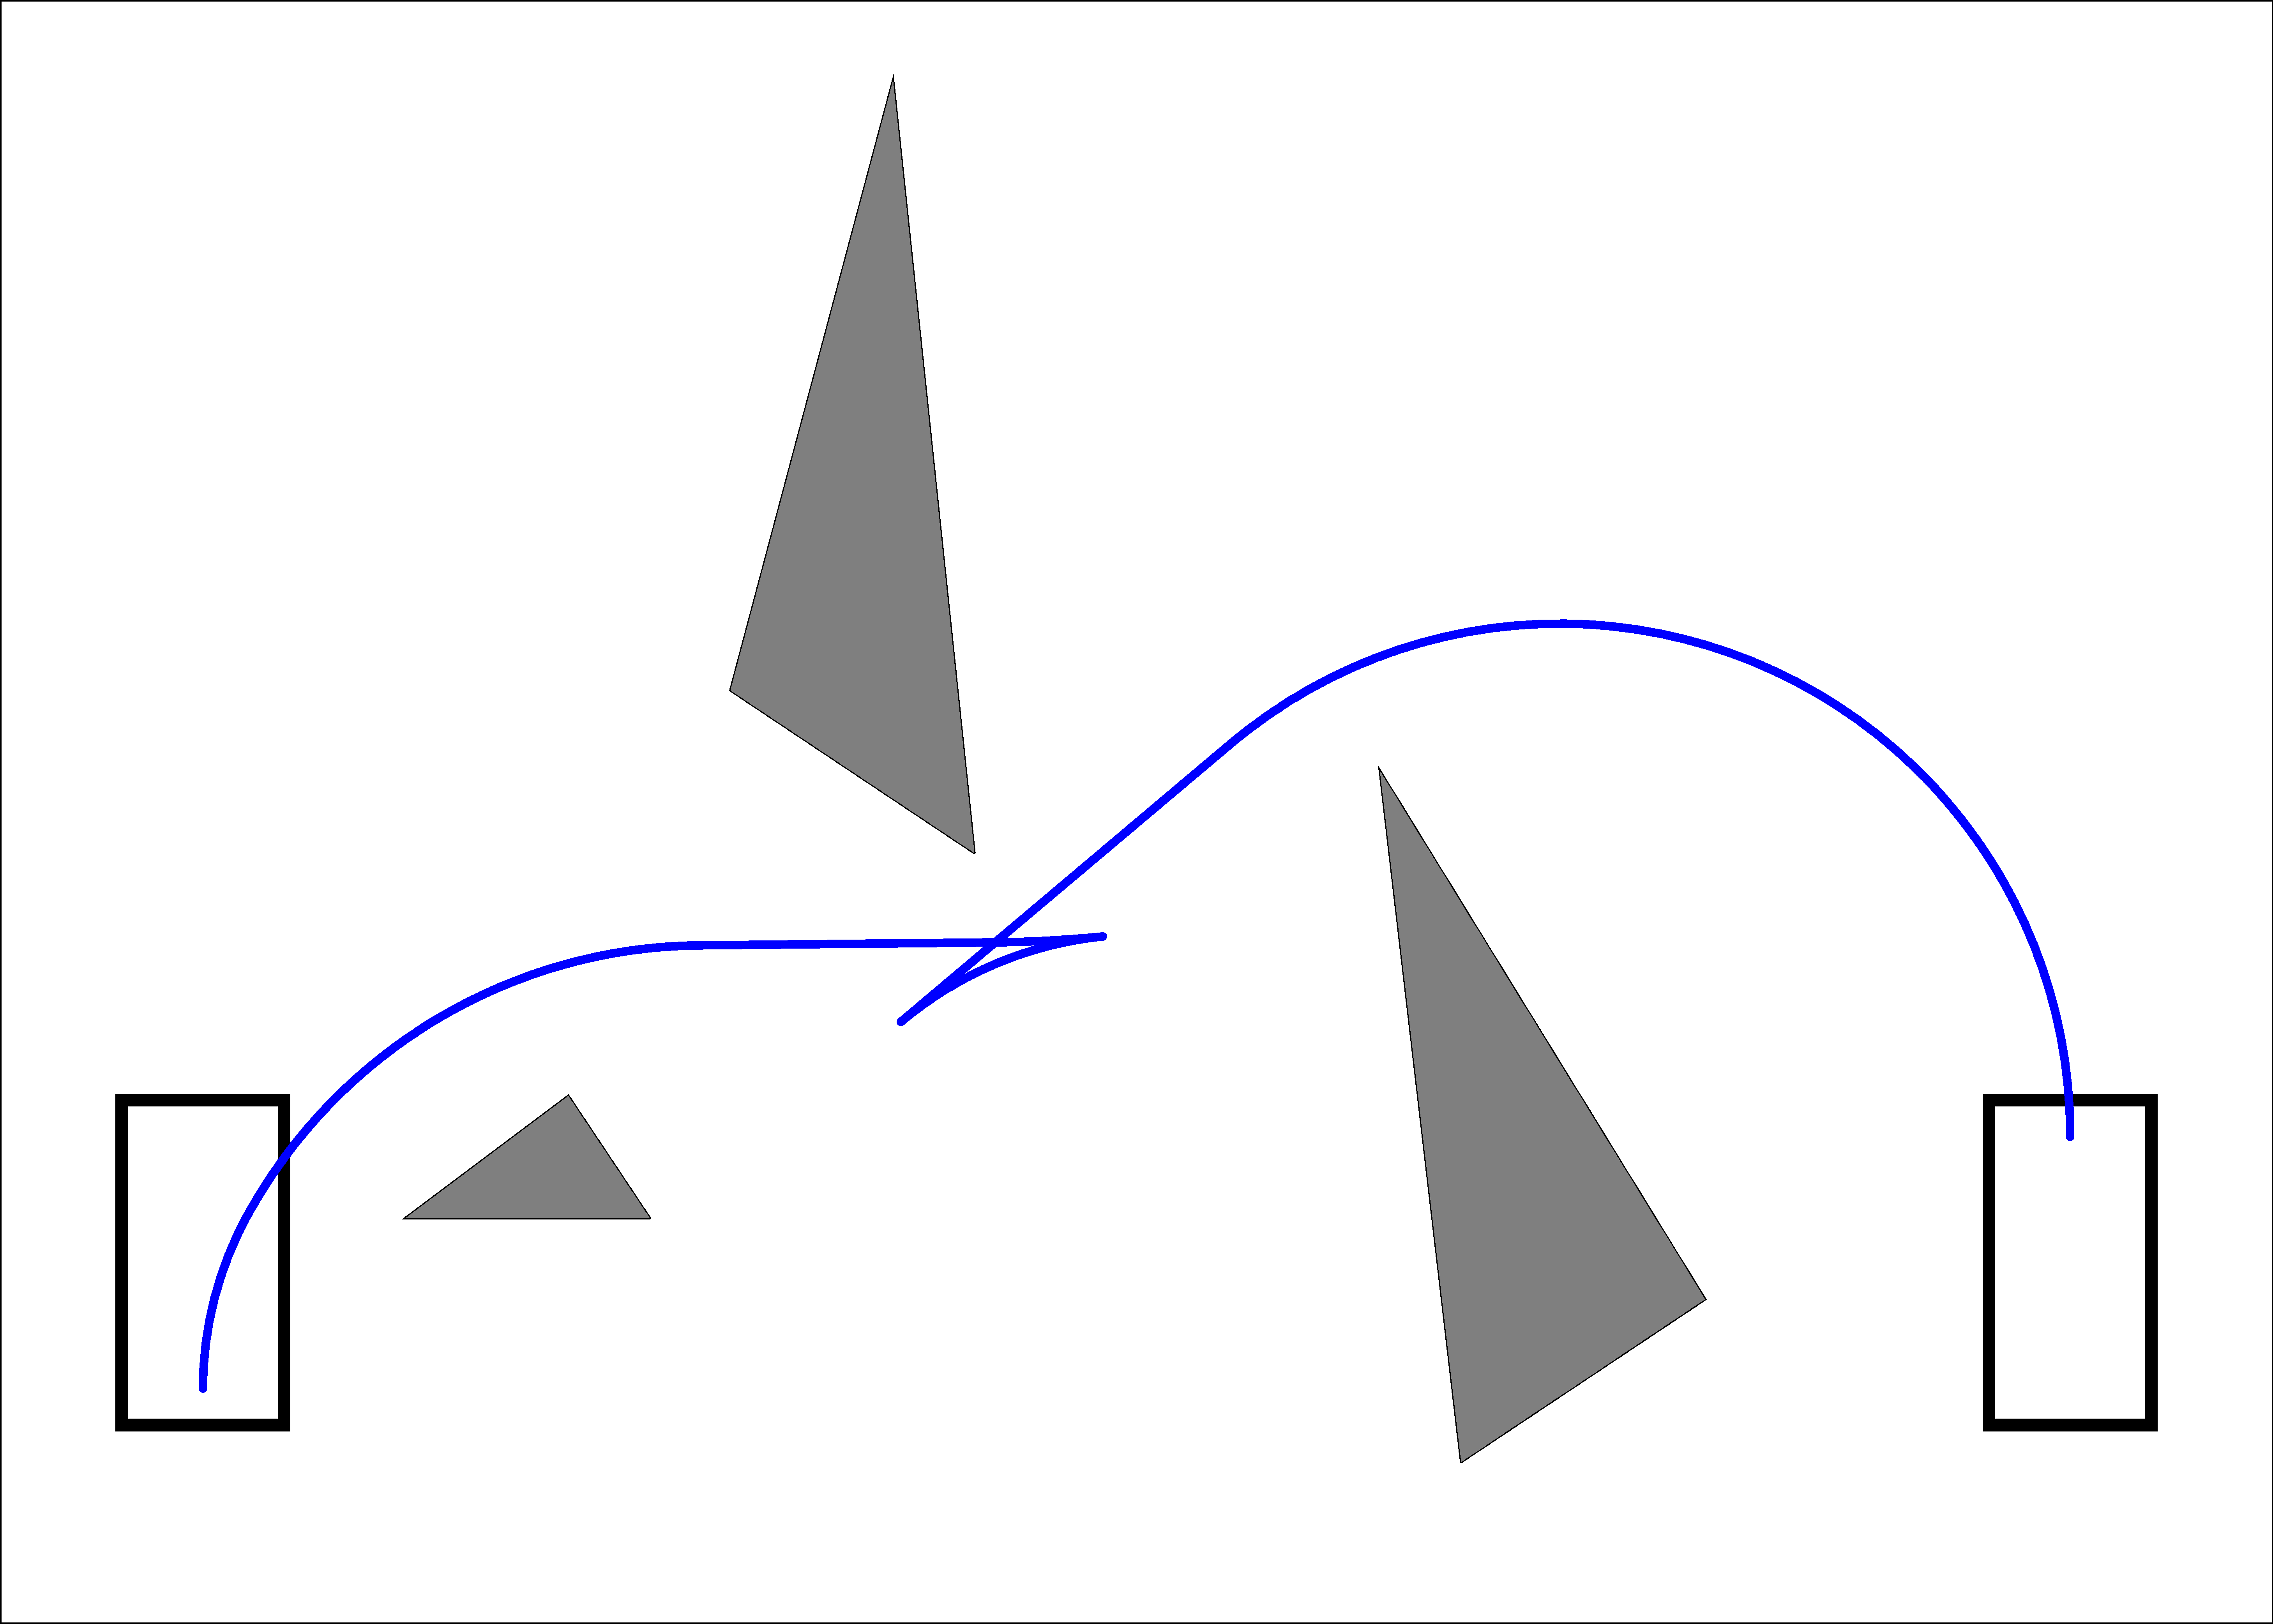
\includegraphics[width=0.49\columnwidth]{.//figures/StaticSim/frameFreeSteering.pdf}
    \label{subfig:frameFreeSteering}}}
    \centerline{
    \subfloat[]{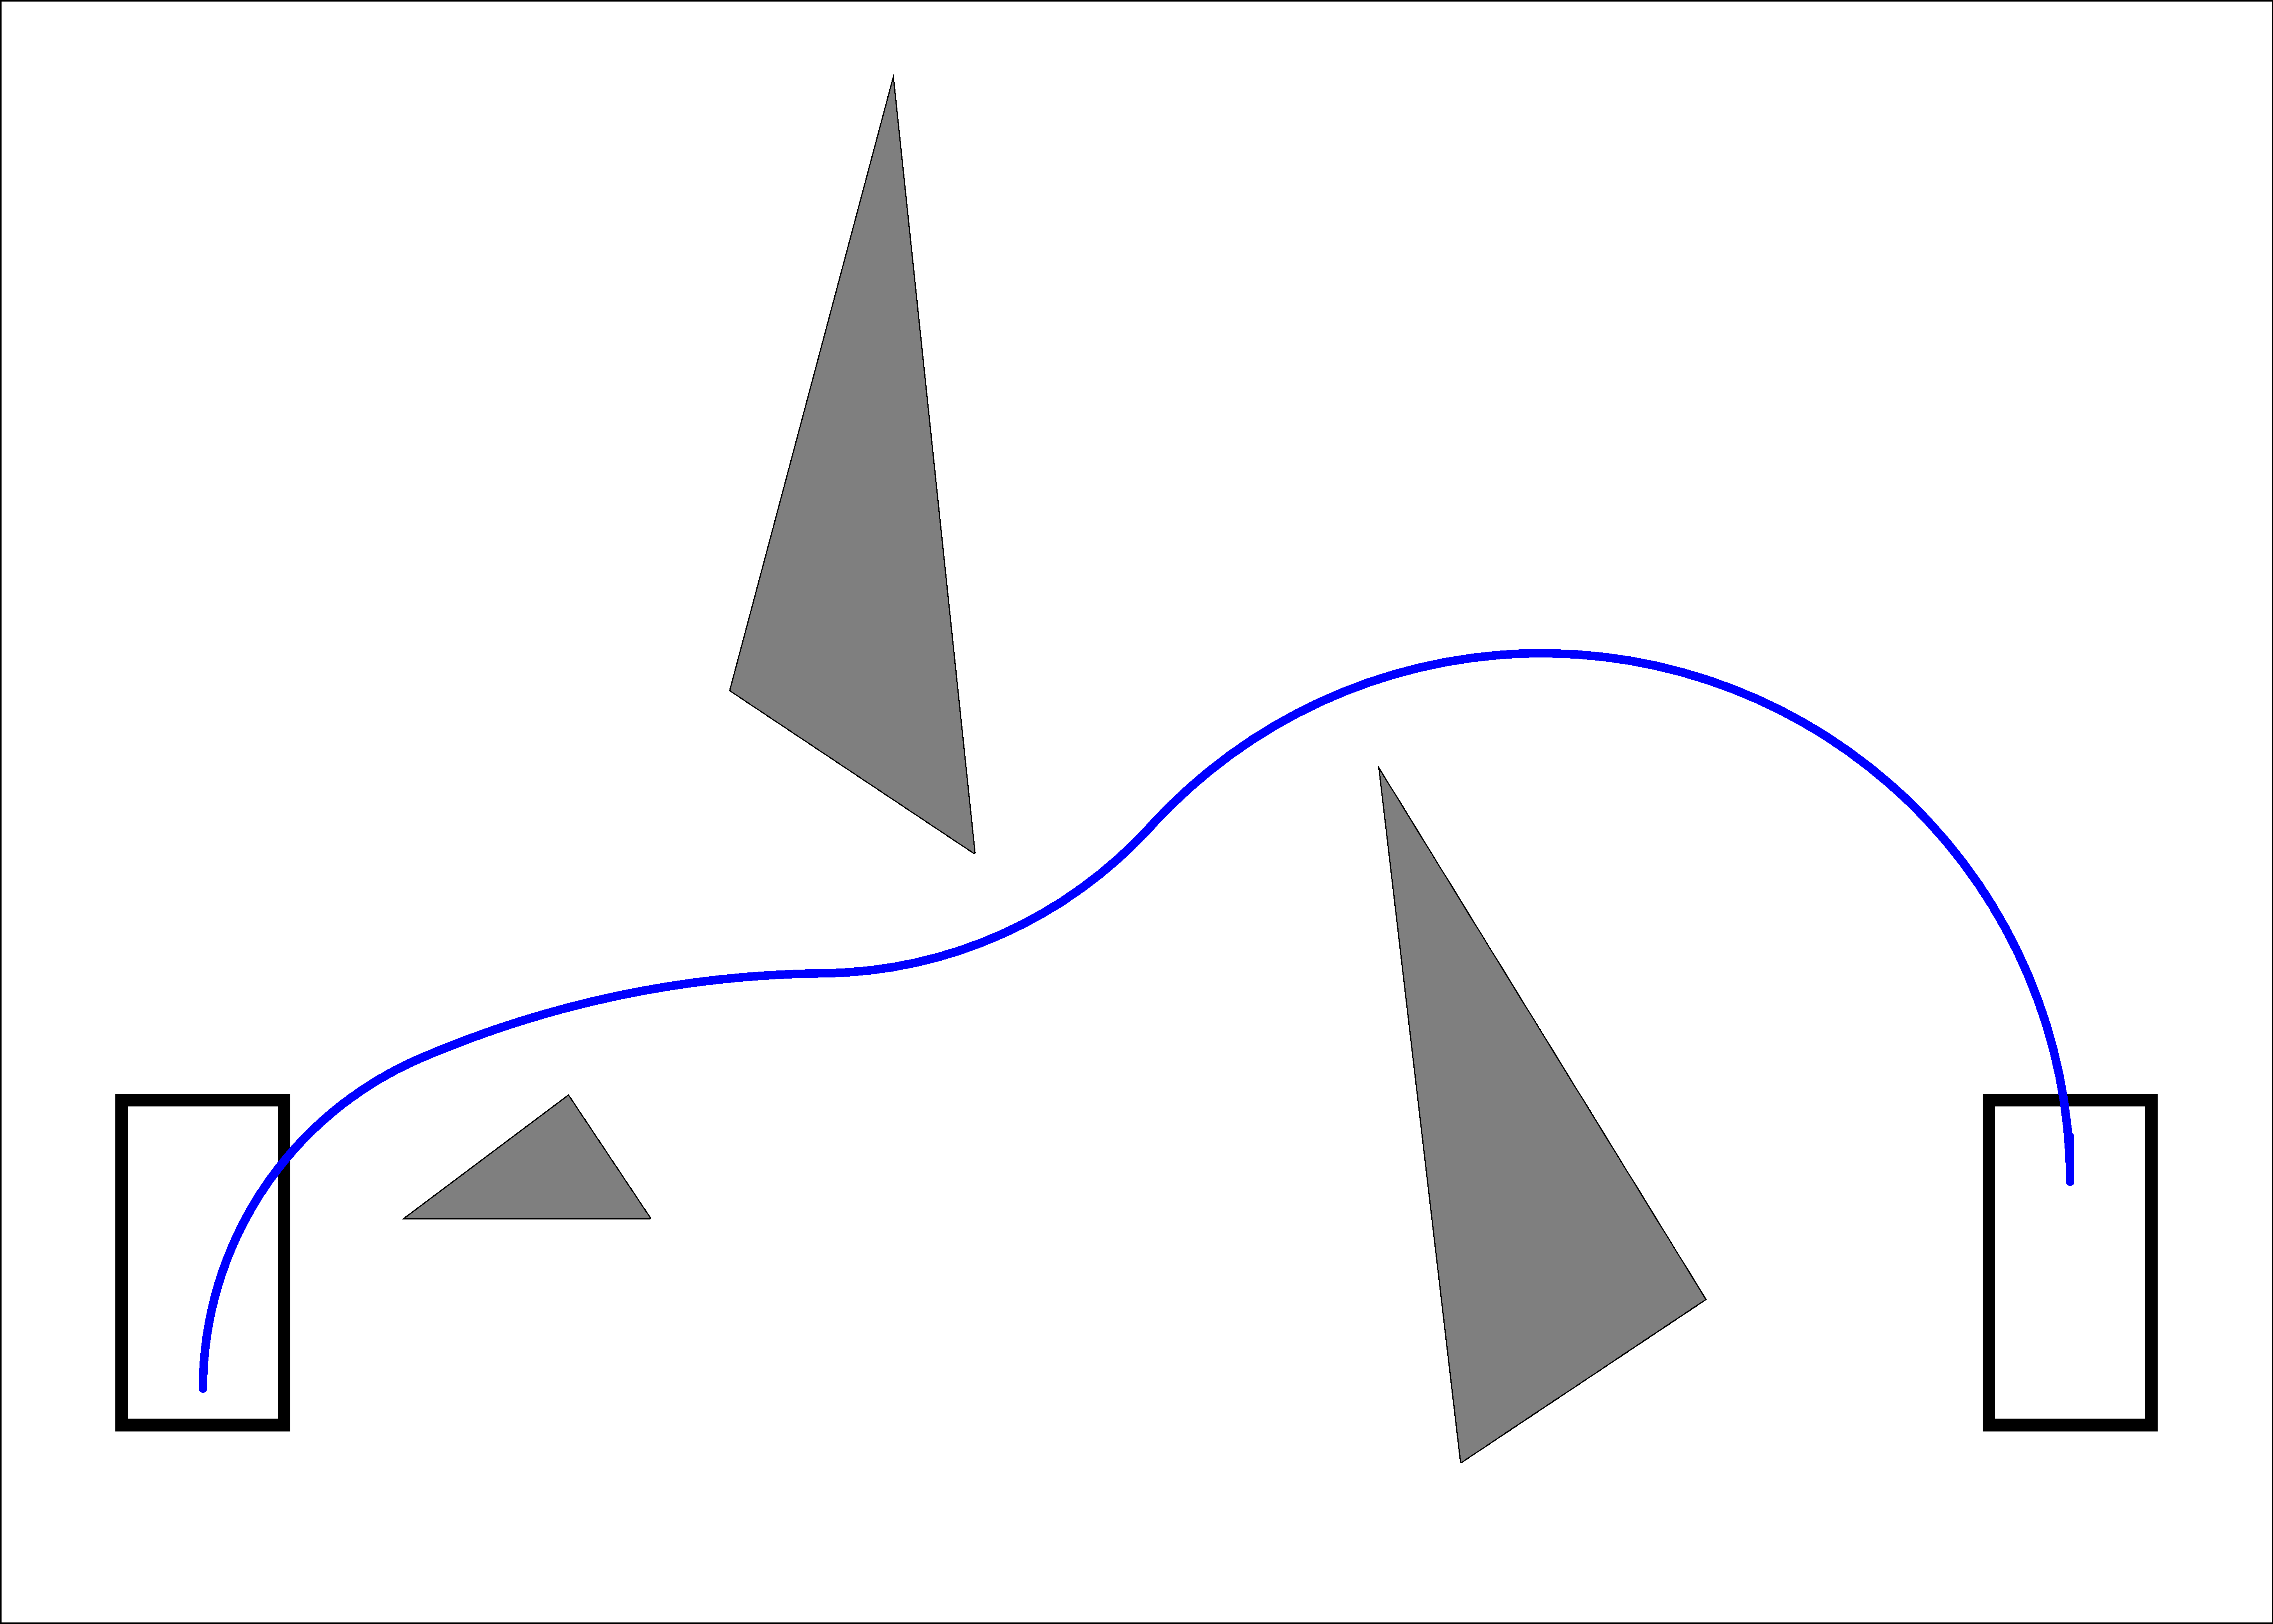
\includegraphics[width=0.49\columnwidth]{.//figures/StaticSim/frameFreeTravel.pdf}
    \label{subfig:frameFreeTravel}}
    \hfil
    \subfloat[]{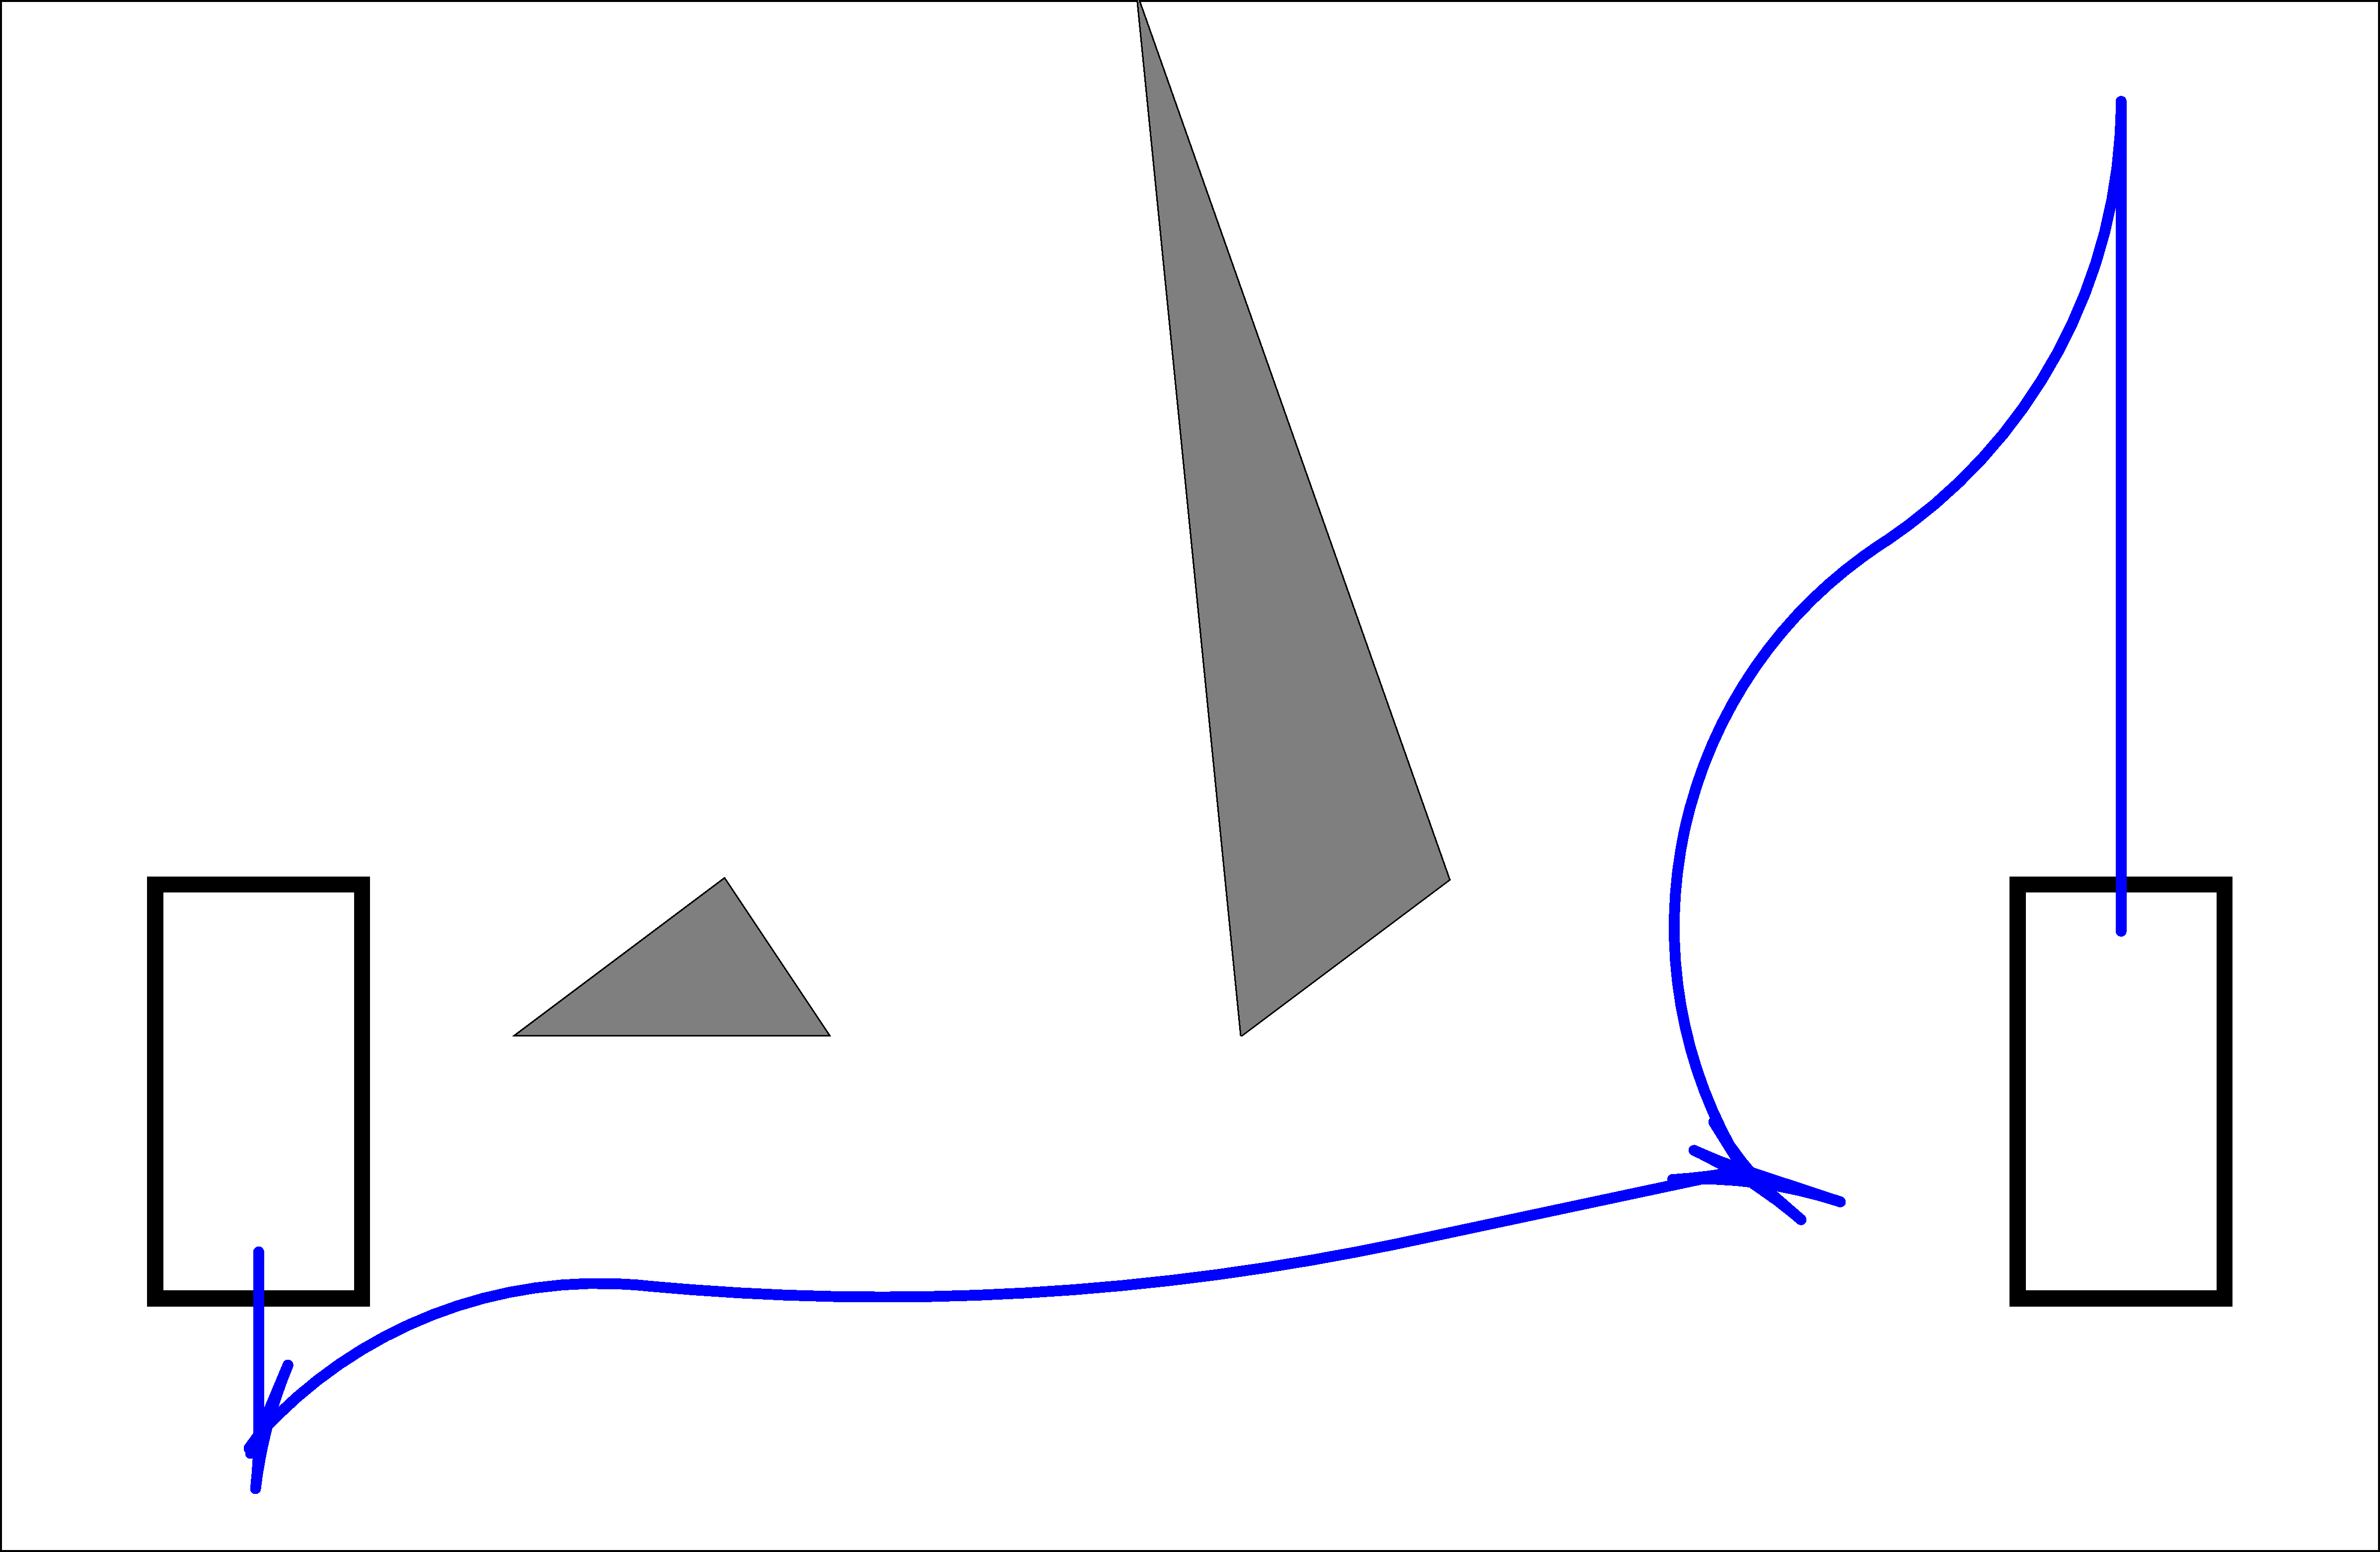
\includegraphics[width=0.49\columnwidth]{.//figures/StaticSim/frameFreeClearance.pdf}
    \label{subfig:frameFreeClearance}}}    
    \caption{Different paths according to different parameters.}
    \label{fig:staticSimTypes}
\end{figure}

\section{Improvements of the final path}
\label{sec:static}

In some cases the final paths are feasible but overly complicated to perform, because the random nature of the previous algorithms it contains too many short manoeuvres or drives too close to the edge of the obstacles \cite{gcsorvasi15iccc}. Our goal was to create paths which are closer to the one which a human driver would plan.

In our previous work we compared different planning methods, and for this we introduced a way to measure the ``quality'' of the resulted path. In the following the same metric is used to characterise our paths and to define a ``fine'' path:

\begin{itemize}
	\item \emph{No. of cusps}: The number of reversals along the path. 
	\item \emph{Steering amount}: The absolute integral of the path curvature.
	\item \emph{Travel time}: The estimated time of driving along the resulting path.
	\item \emph{Average clearance}: The average clearance from the obstacles along the path.
\end{itemize}

For a passenger could be too many reversals uncomfortable same as if the amount of turning along the path is too high. The travel time is estimated as follows. A travelling speed function with $v_{max} = 5\frac{m}{s}$ and $v_{min} = 1\frac{m}{s}$ is assigned to the path, which is inversely proportional to the actual path curvature. The cusps are penalized with $0.5s$ ``reversing time''. Those paths are better, which requires less time to travel along.

In addition to the formerly used qualities the average clearance is added as well. To specify the clearance the path is sampled. For each sample point the minimal distance from the obstacles is calculated and summarized. At last the sum is normalized with the length of the path. The purpose of this parameter is to keep the robot keep away from the obstacles as a real driver would do to protect the car.

Examples can be seen in \figurename~\ref{fig:staticSimTypes}. In this scenario the robot starts from the left position facing upwards and the goal position is on the right facing down. In \figurename~\ref{subfig:frameFreeCusps} the number of cusps are minimal. As shown in \figurename~\ref{subfig:frameFreeSteering} the steering amount is minimized, the straighter paths are preferred. In \figurename~\ref{subfig:frameFreeTravel} the resulted path is shorter, but it consumes less time to travel along. At last the path in \figurename~\ref{subfig:frameFreeClearance} is more complicated than the others, but the obstacles are avoided.

In order to tune the final path the planning algorithm was executed several times with different global paths and the above detailed parameters were normalized between the $[0,1]$ interval and multiplied with a weight factor.

\begin{figure}[tb]
    \centerline{
    \subfloat[]{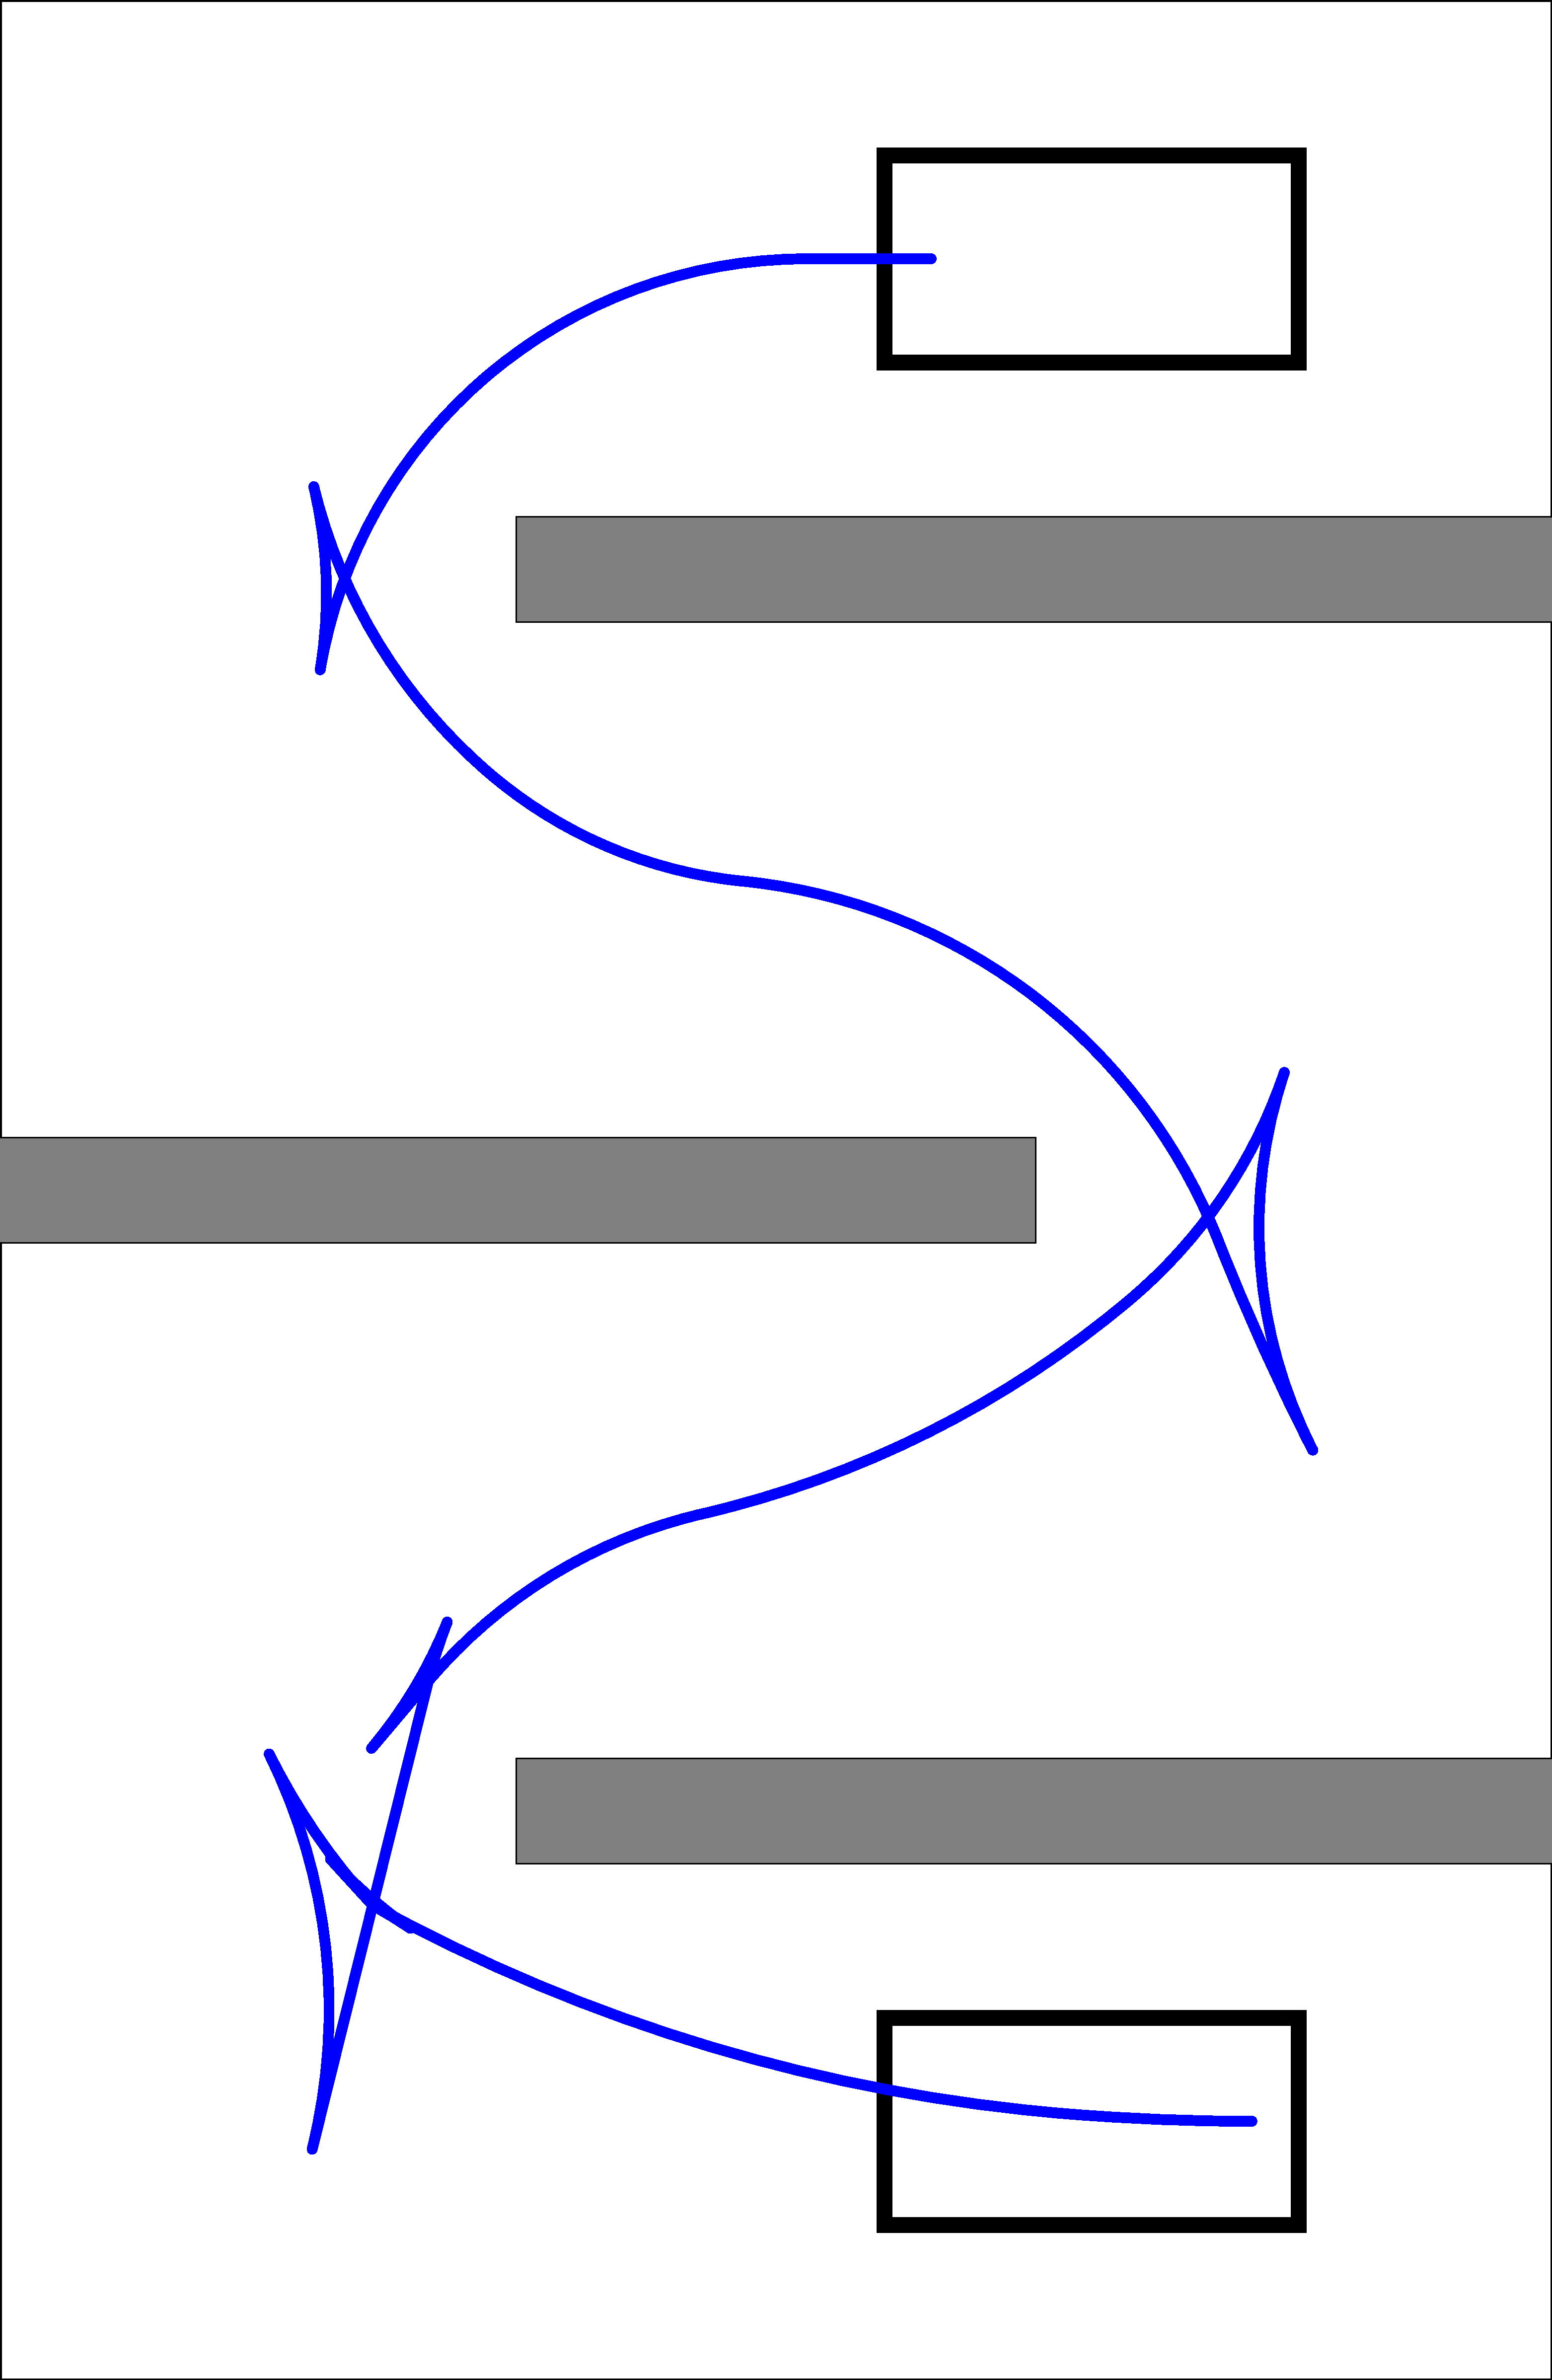
\includegraphics[width=0.40\columnwidth]{.//figures/StaticSim/frame2SC.pdf}
    \label{subfig:static2SC}}%}
    \hfil
	%\centerline{
    \subfloat[]{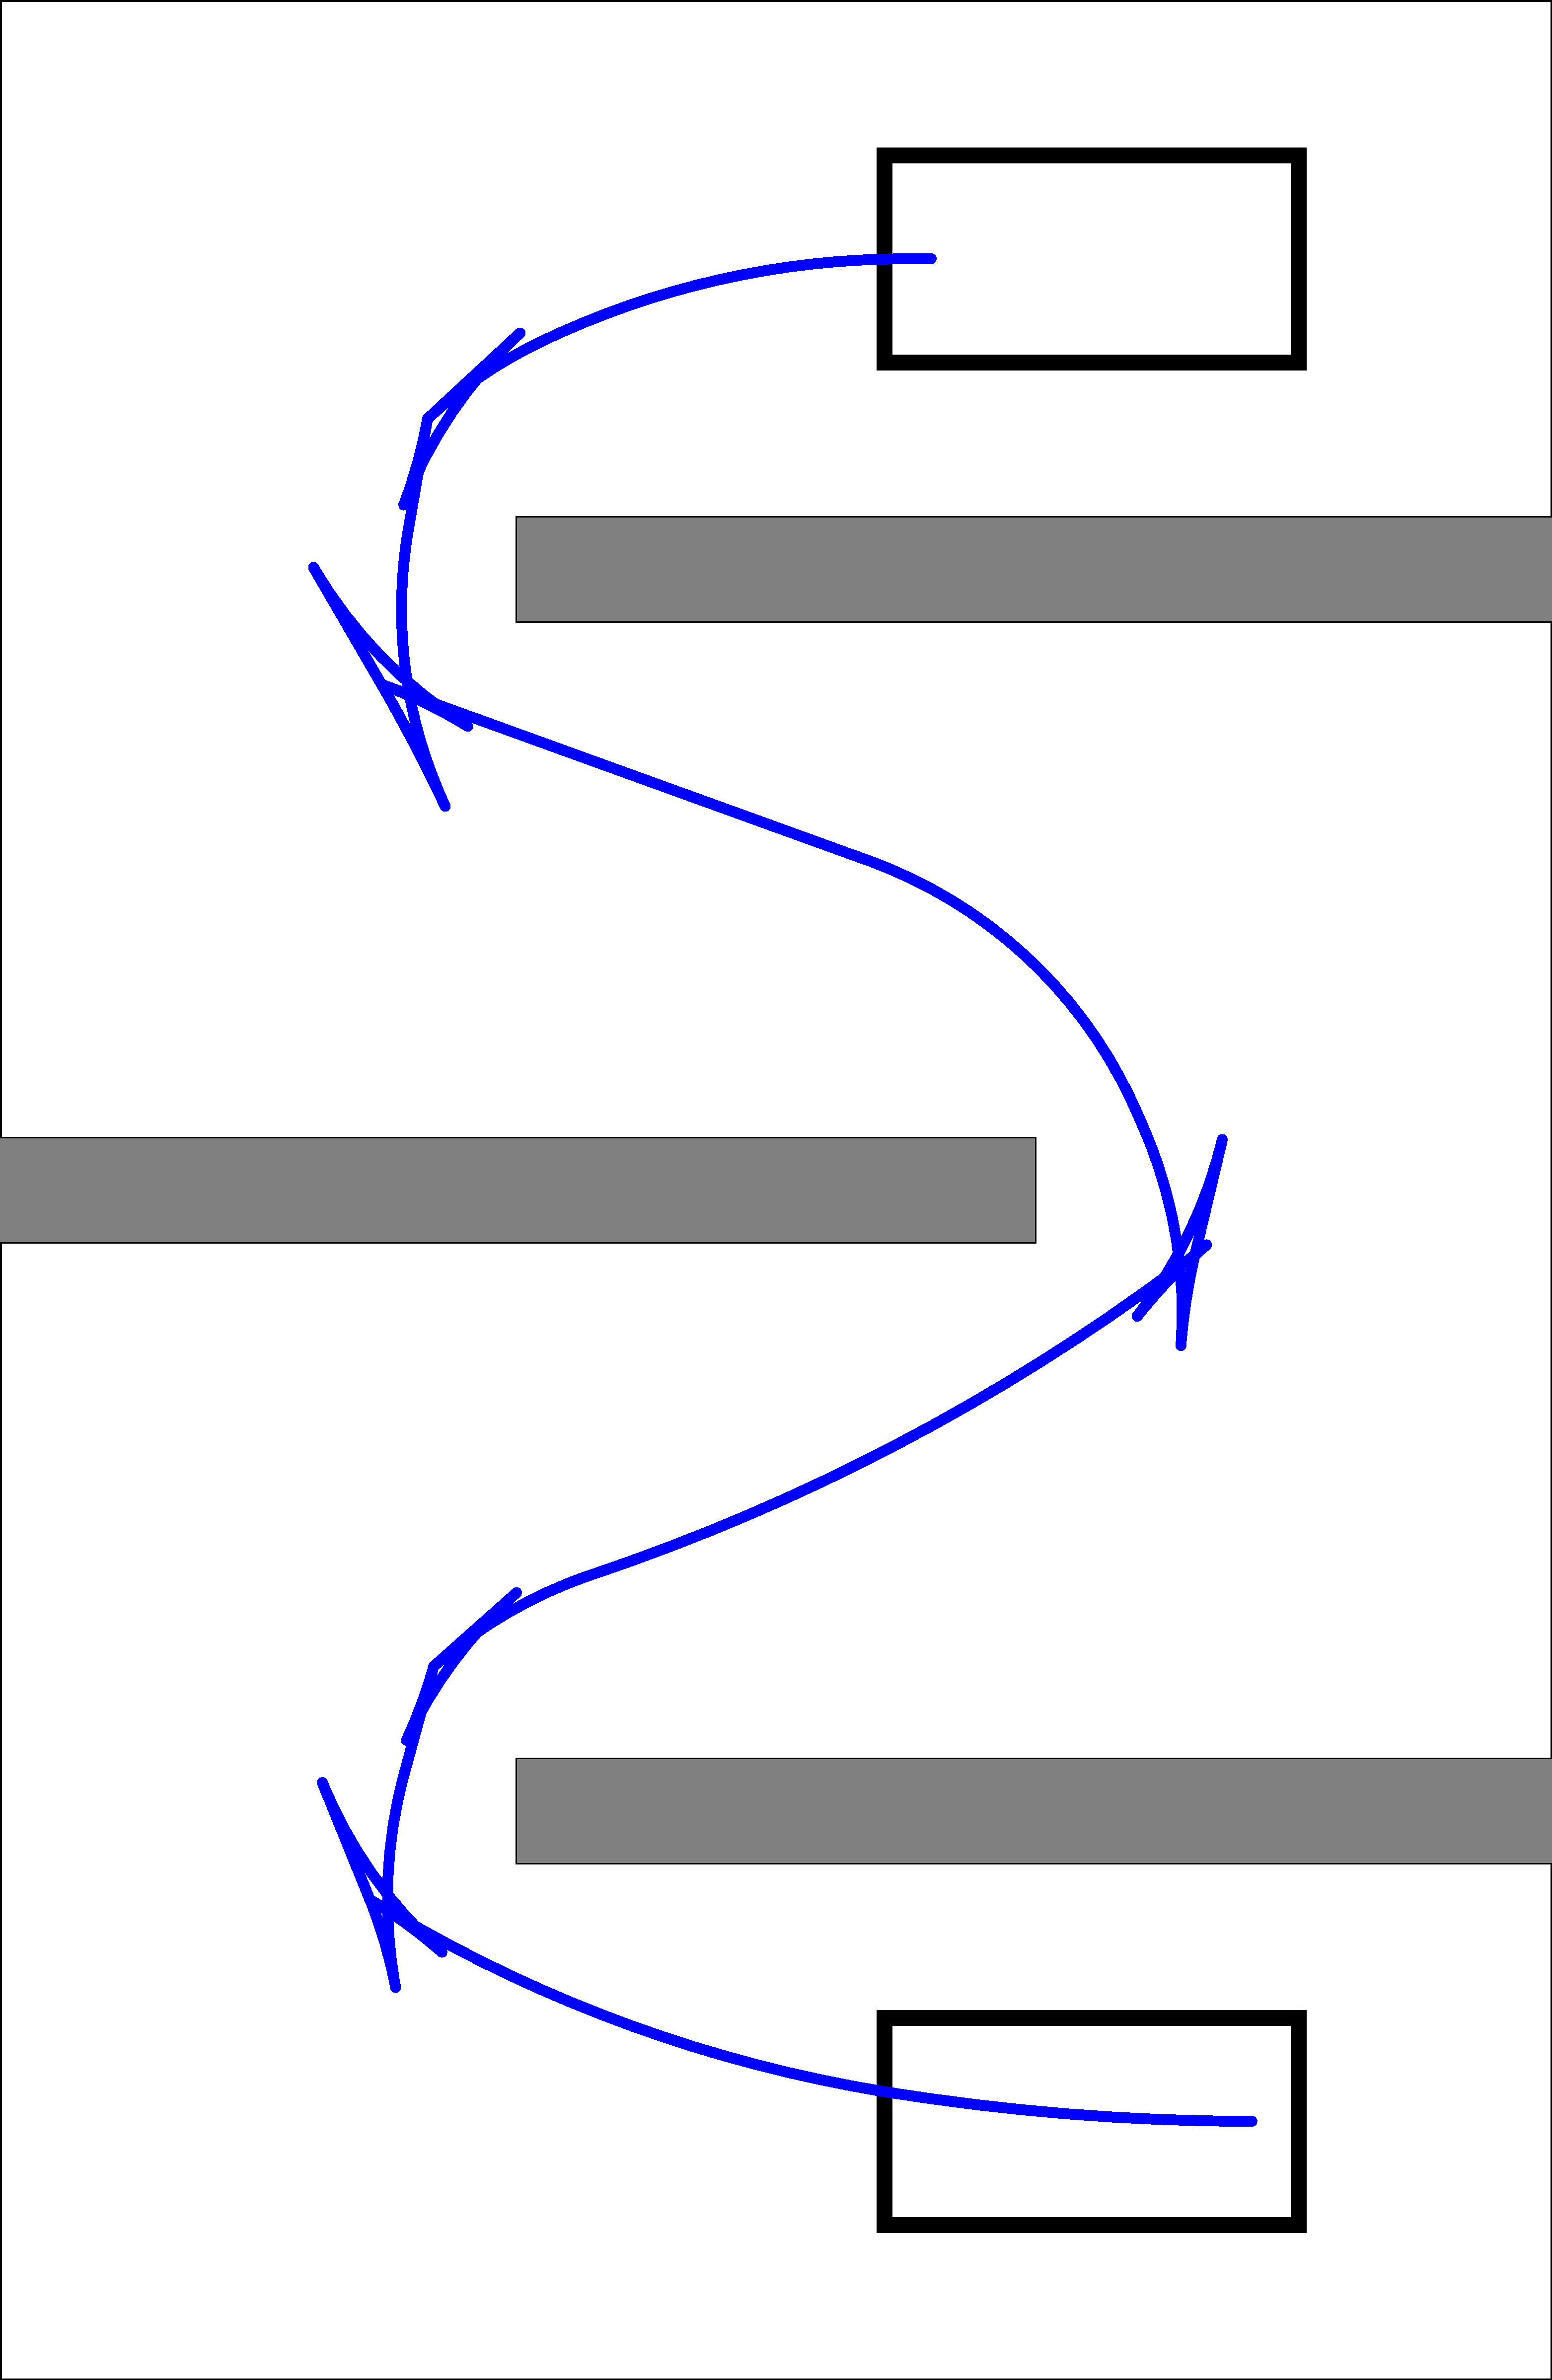
\includegraphics[width=0.40\columnwidth]{.//figures/StaticSim/frame2ST.pdf}
    \label{subfig:static2ST}}}
    \centerline{
    \subfloat[]{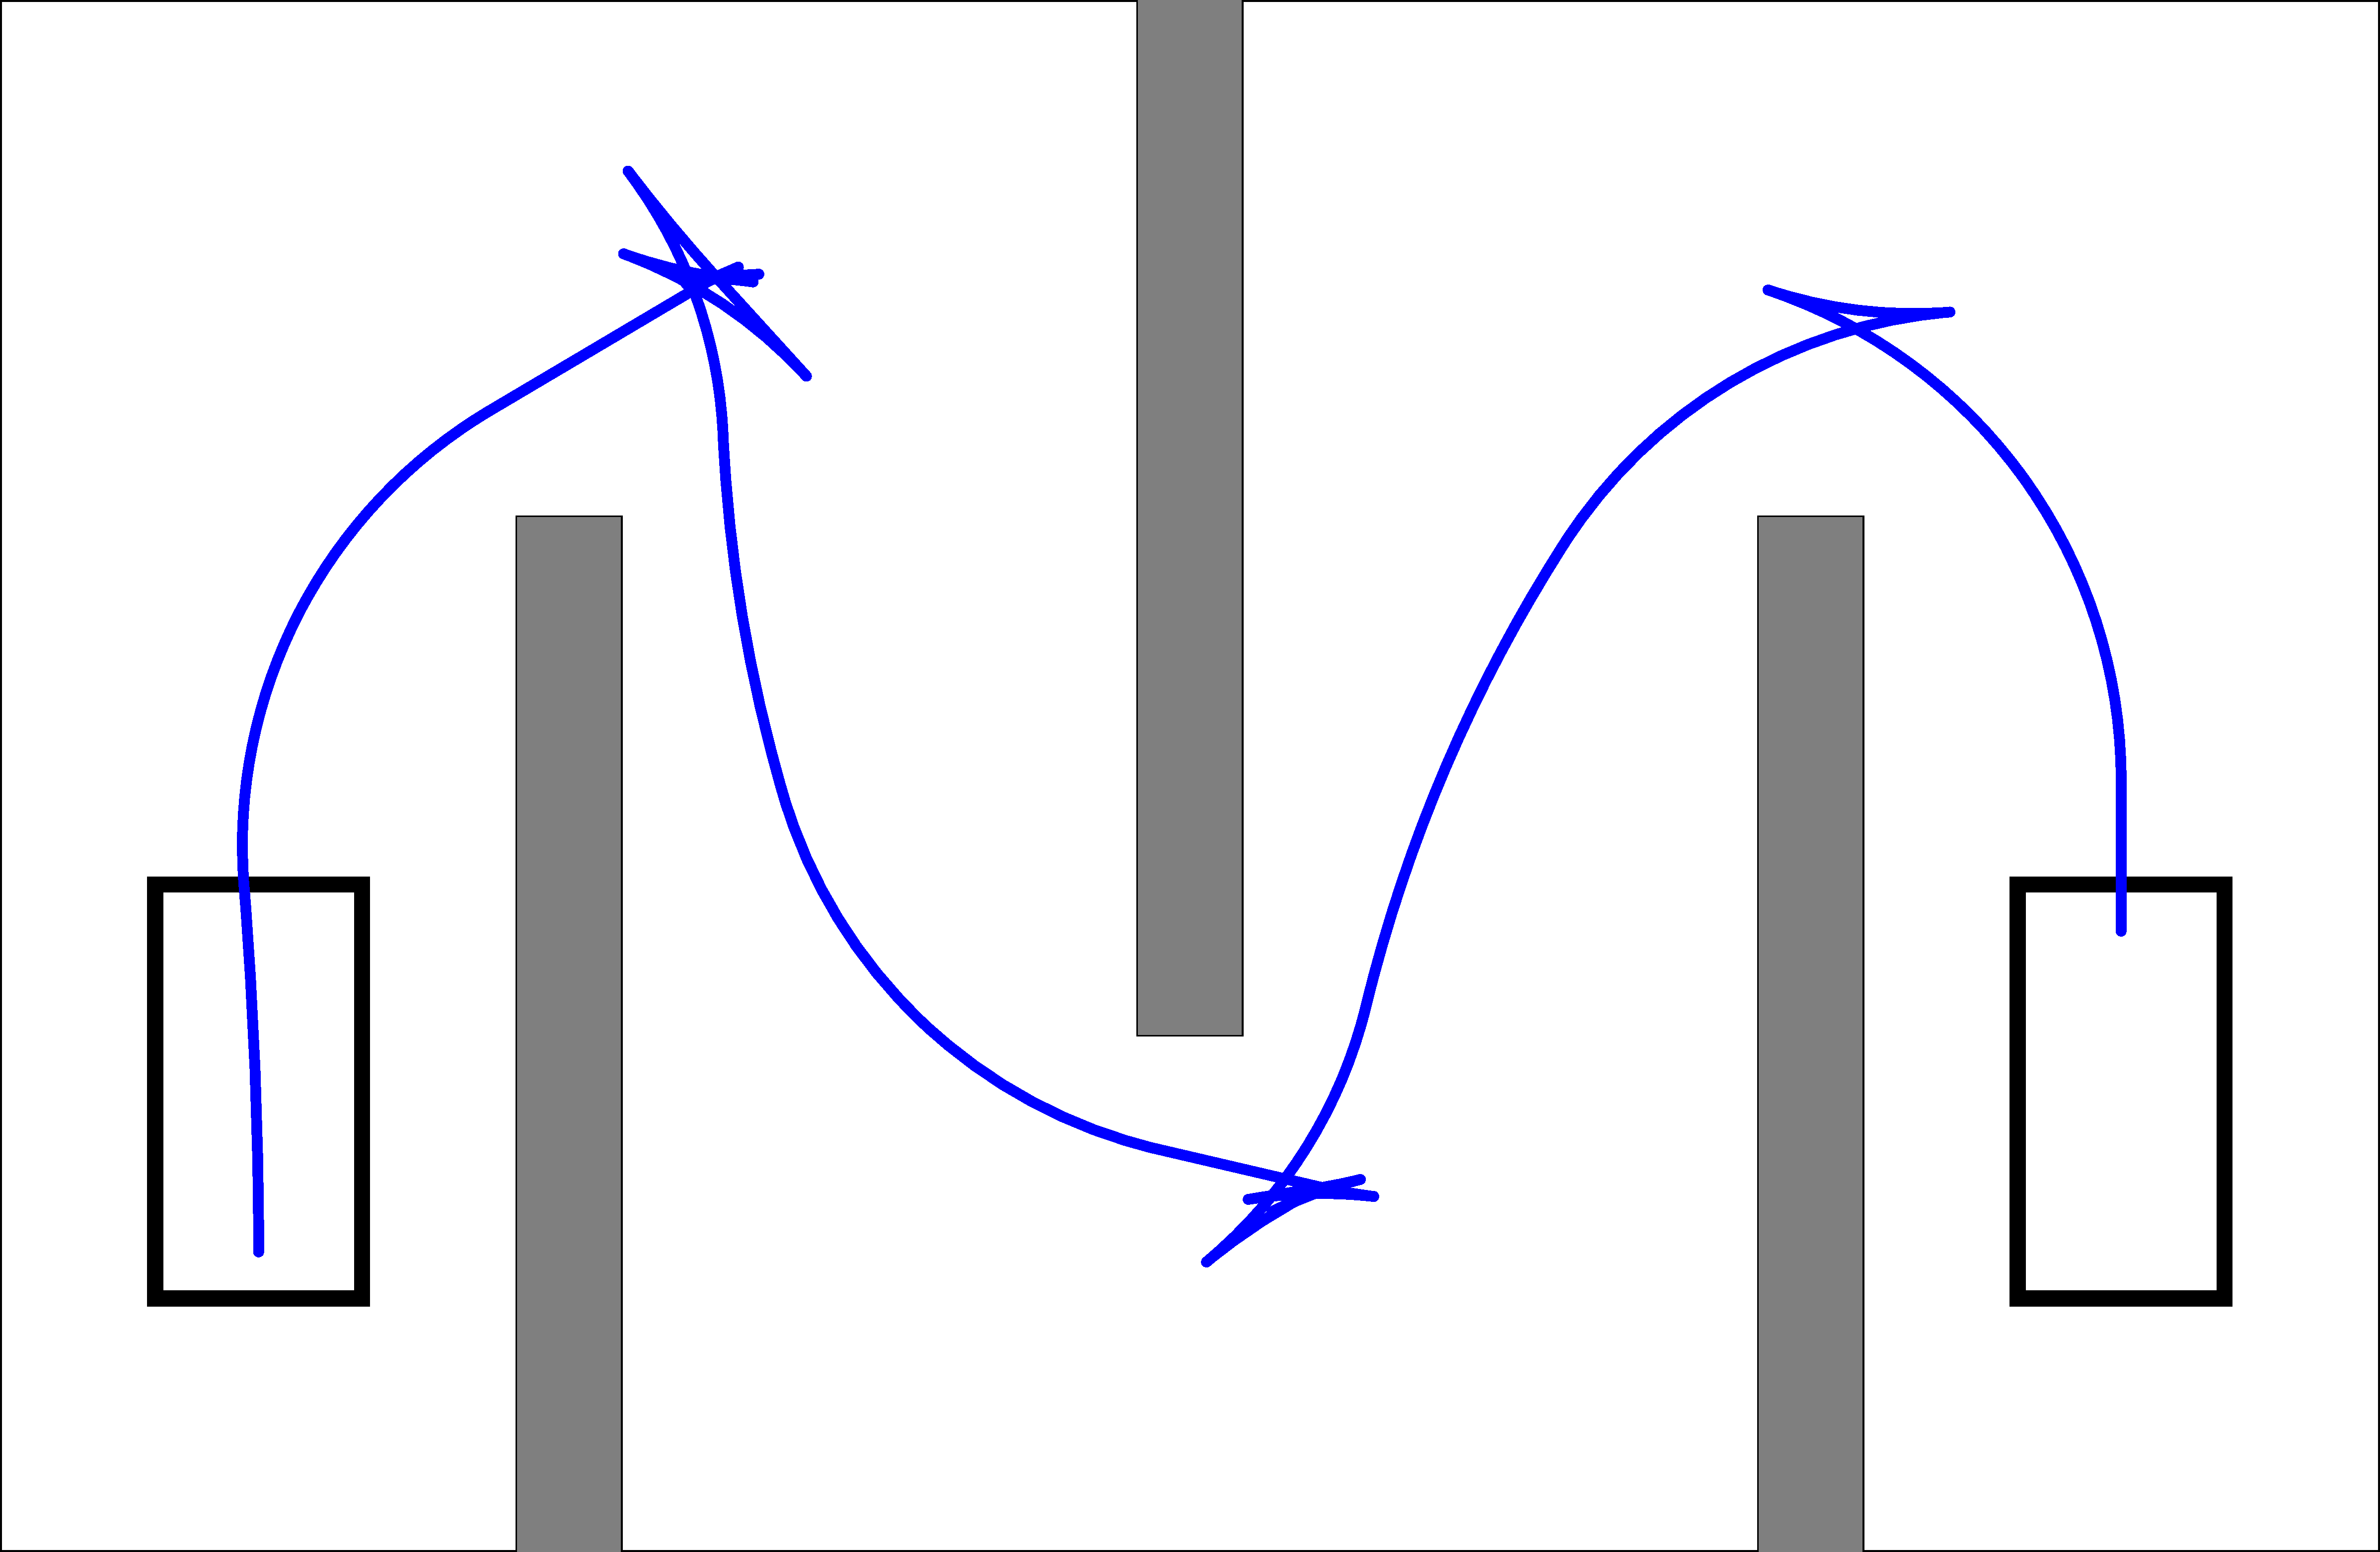
\includegraphics[width=0.65\columnwidth]{.//figures/StaticSim/frame2CTC.pdf}
    \label{subfig:static2CTC}}}
    \caption{Resulted paths in an M-shape environment.}
    \label{fig:staticMShape}
\end{figure}

The weight factors can depend on different scenarios and on individual choice as well. In a narrow M-shaped environment, which is shown in \figurename~\ref{fig:staticMShape}, can be difficult to manoeuvre therefore the resulted paths have similarities, but even in this scenario the differences can be observed. In \figurename~\ref{subfig:static2SC}, \ref{subfig:static2ST} the steering amount is lowered thus the longer path segments have a low curvature. In \figurename~\ref{subfig:static2SC} the weight of cusps is higher (lower cusps number) and in \figurename~\ref{subfig:static2ST} the travel time is shorter. In \figurename~\ref{subfig:static2CTC} the weight factor of cusps, travel time and clearance is increased so the curvature can be higher but the planner algorithm tries to avoid the obstacles.

In a one corridor scenario the differences can be observed easier. In \figurename~\ref{subfig:frame130} the steering amount is low because of the straight middle segment, in \figurename~\ref{subfig:frame146} the cusps number is lowered in order to achieve a simpler path. This path is the best in travel time as well. In \figurename~\ref{subfig:frame153} and \ref{subfig:frame173} the clearance factor is increased. In these situations the car rather uses the larger open spaces to manoeuvre and drives in the middle of the corridor.

In a situation where the planning time is not a serious concern e.g. where the resulted path could be reused or the ``quality'' of the resulted path is important the above detailed method could be a suitable choice.

\begin{figure}[tb]
    \centerline{
    \subfloat[]{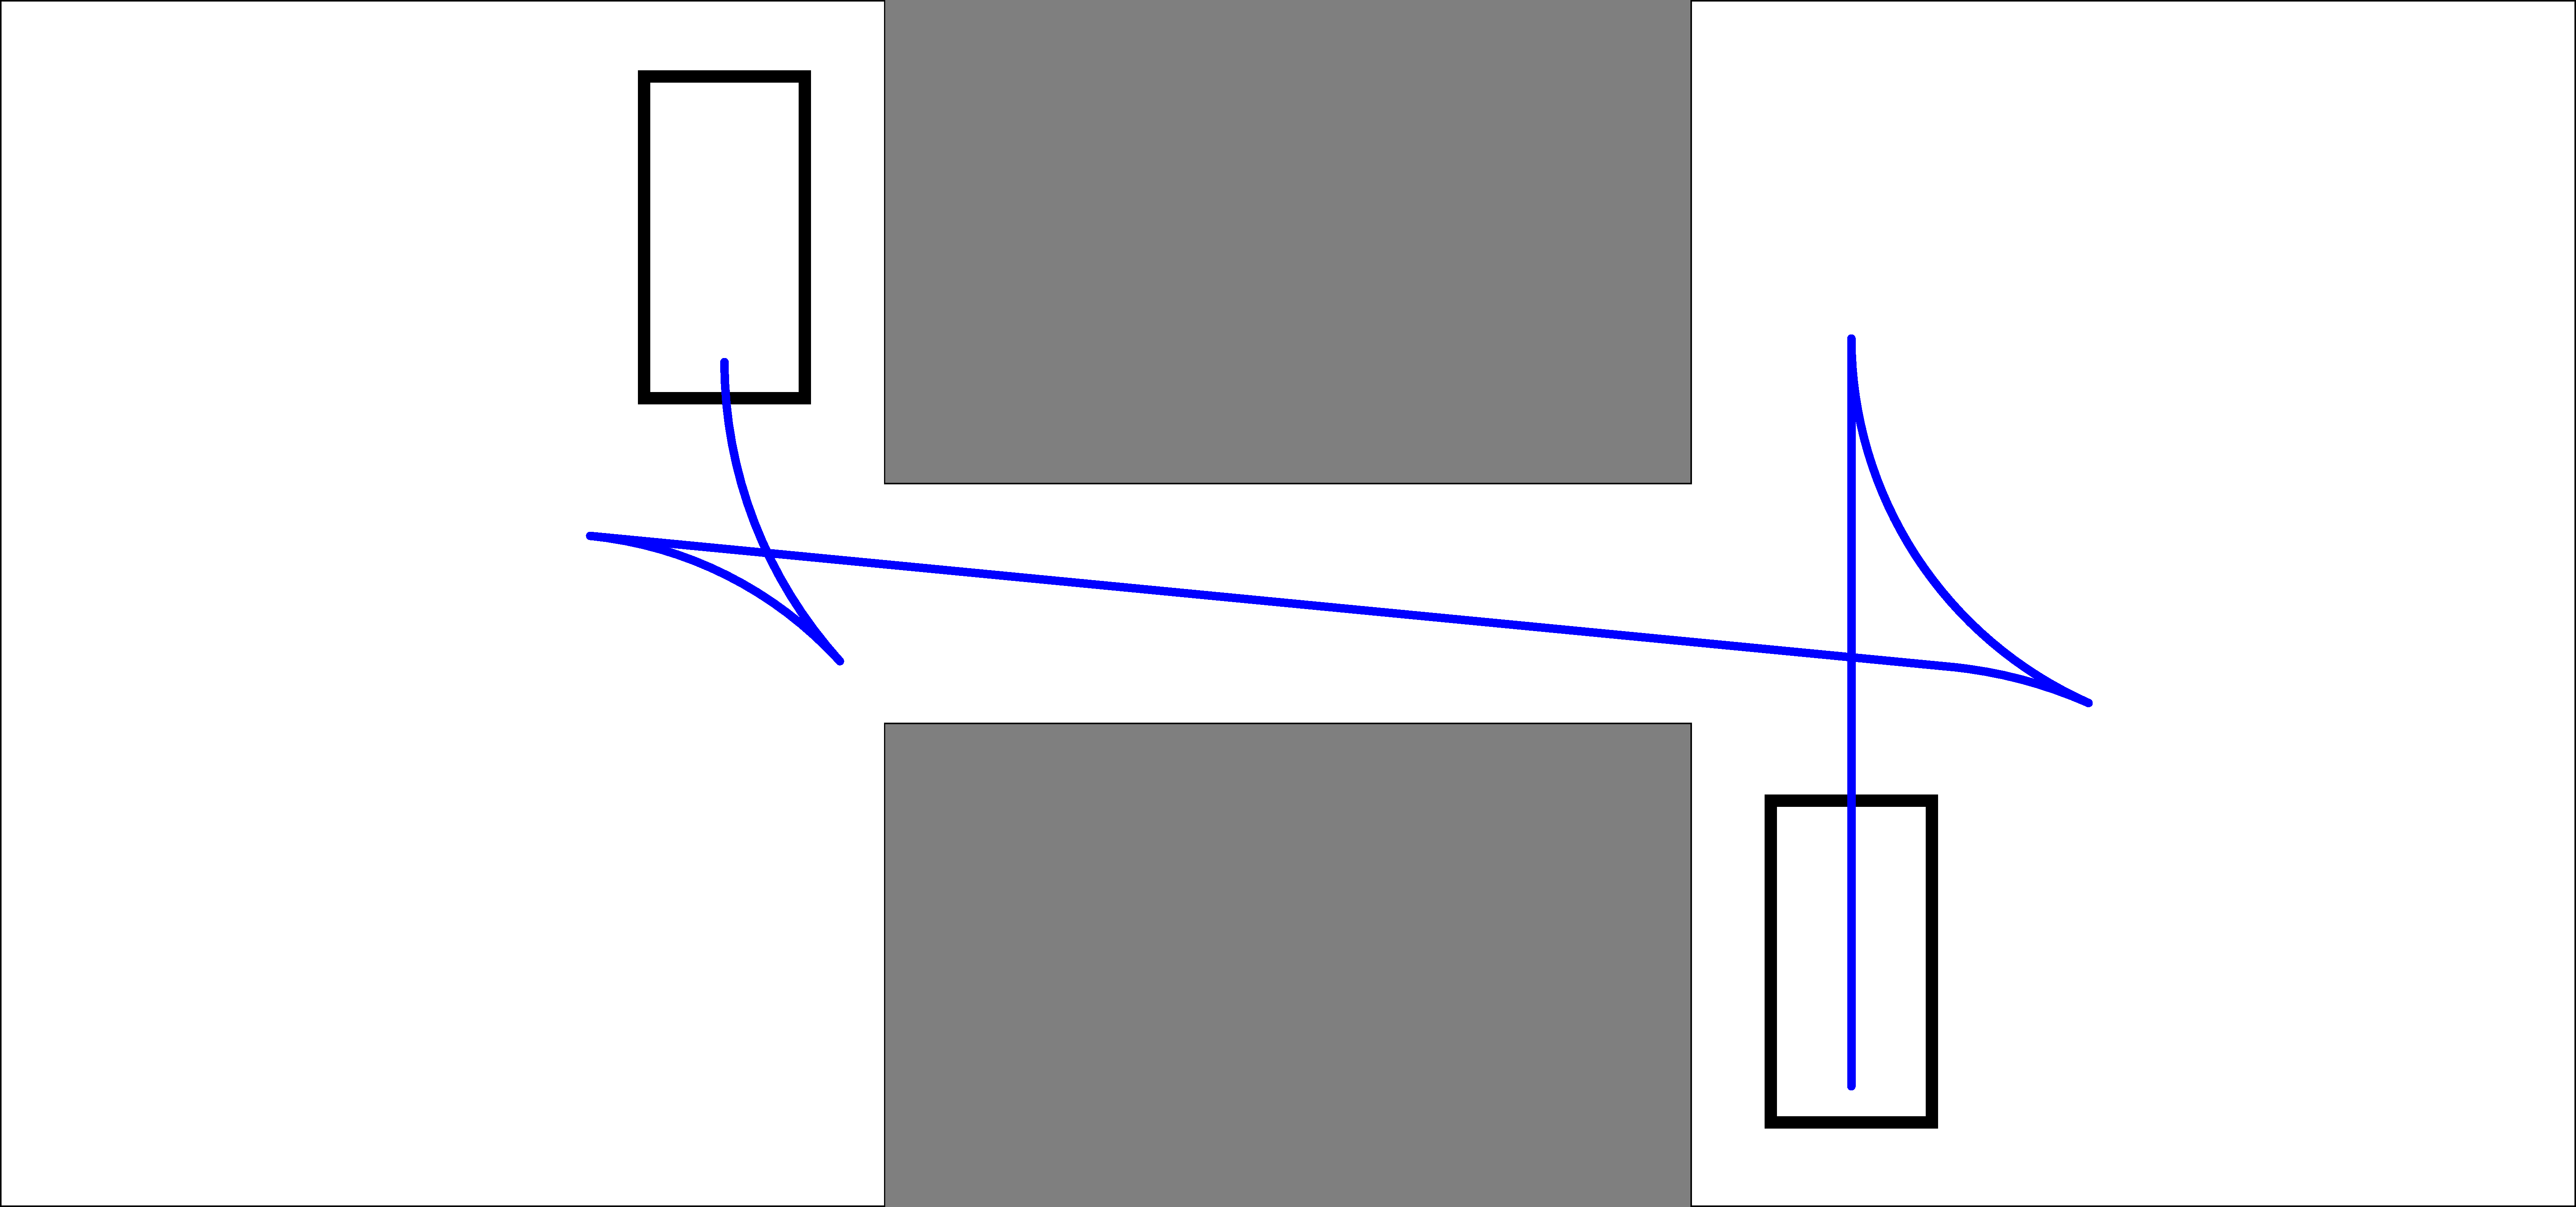
\includegraphics[height=0.35\columnwidth]{.//figures/StaticSim/frame130.pdf}
    \label{subfig:frame130}}}
    \centerline{
    \subfloat[]{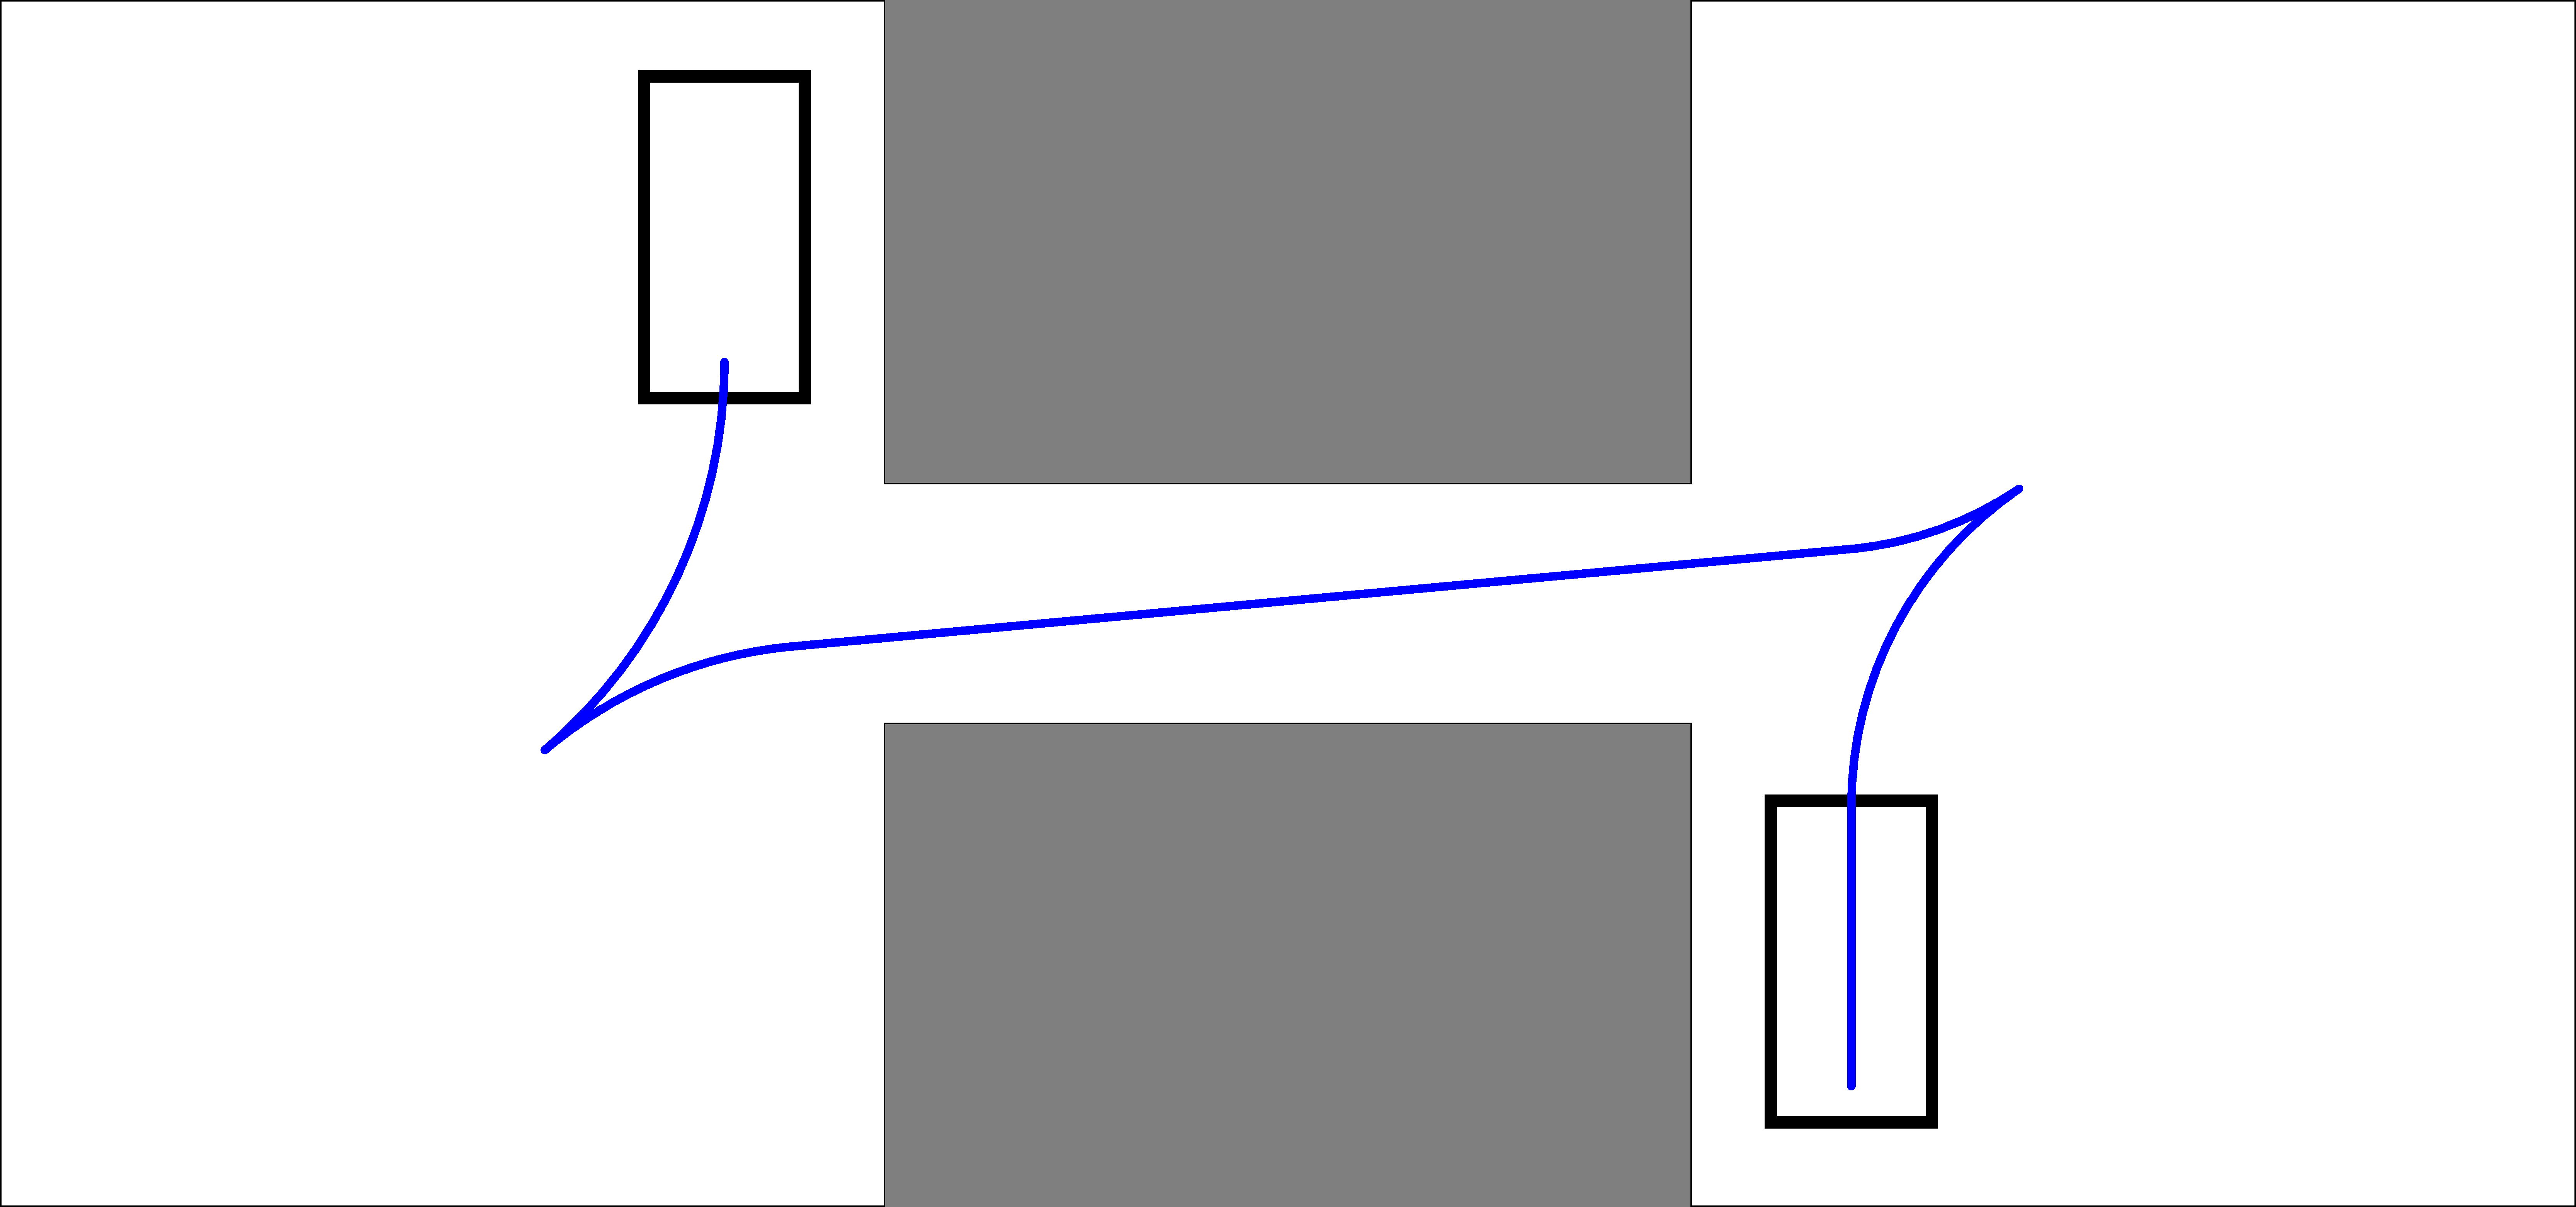
\includegraphics[height=0.35\columnwidth]{.//figures/StaticSim/frame146.pdf}
    \label{subfig:frame146}}}
    \centerline{
    \subfloat[]{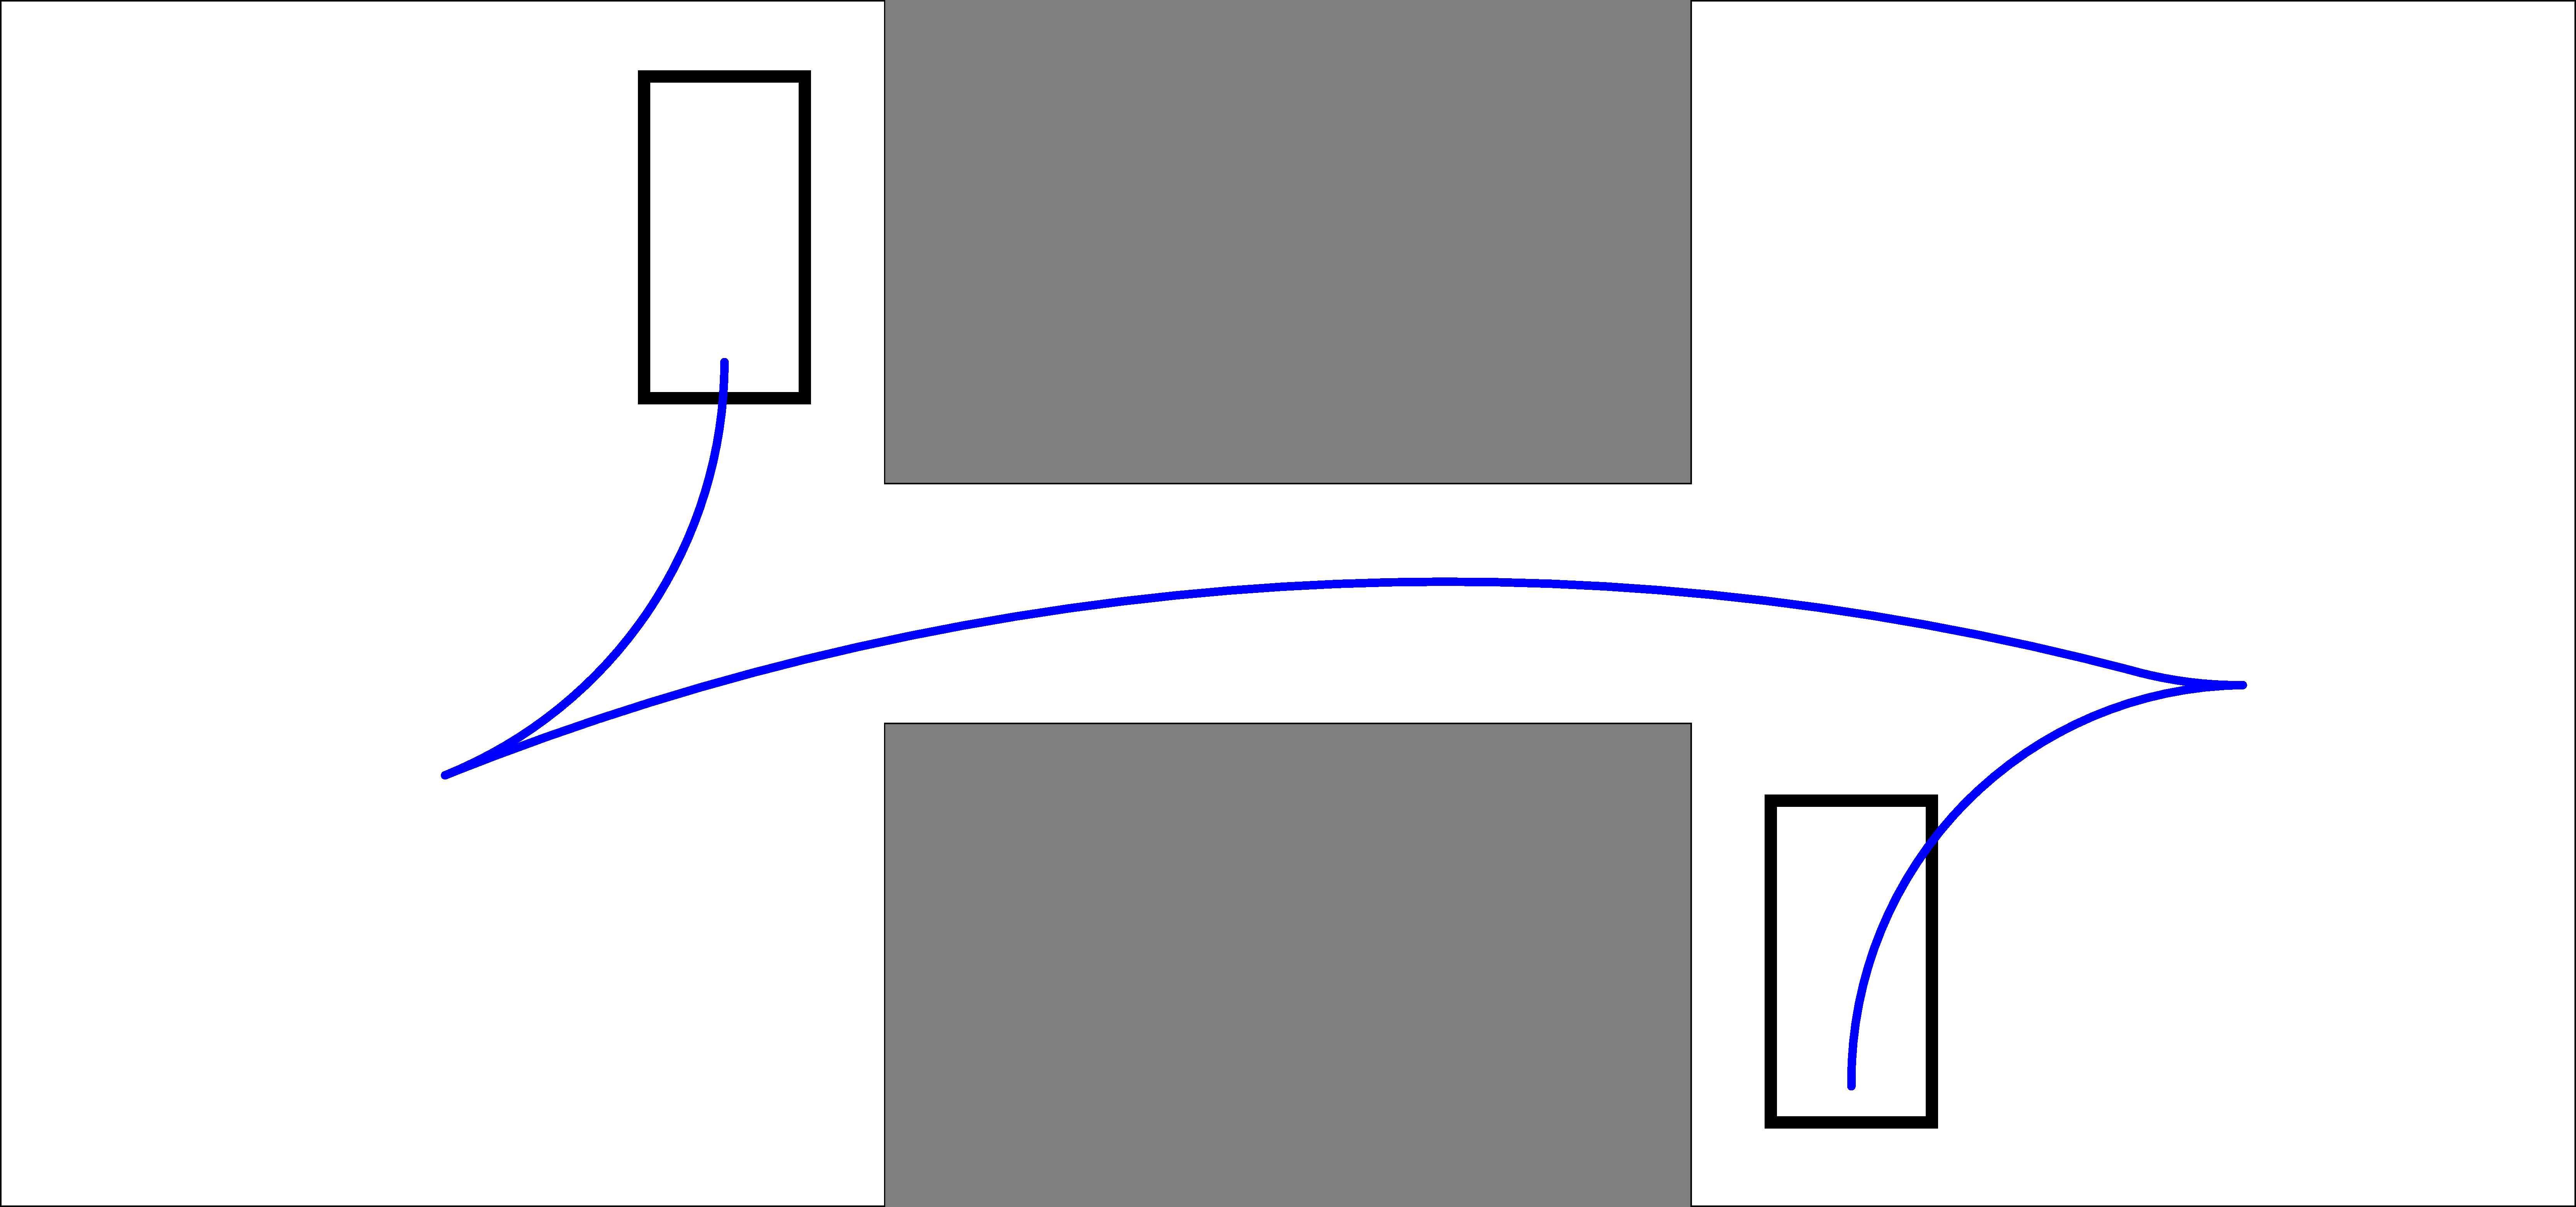
\includegraphics[height=0.35\columnwidth]{.//figures/StaticSim/frame153.pdf}
    \label{subfig:frame153}}}    
    \centerline{
    \subfloat[]{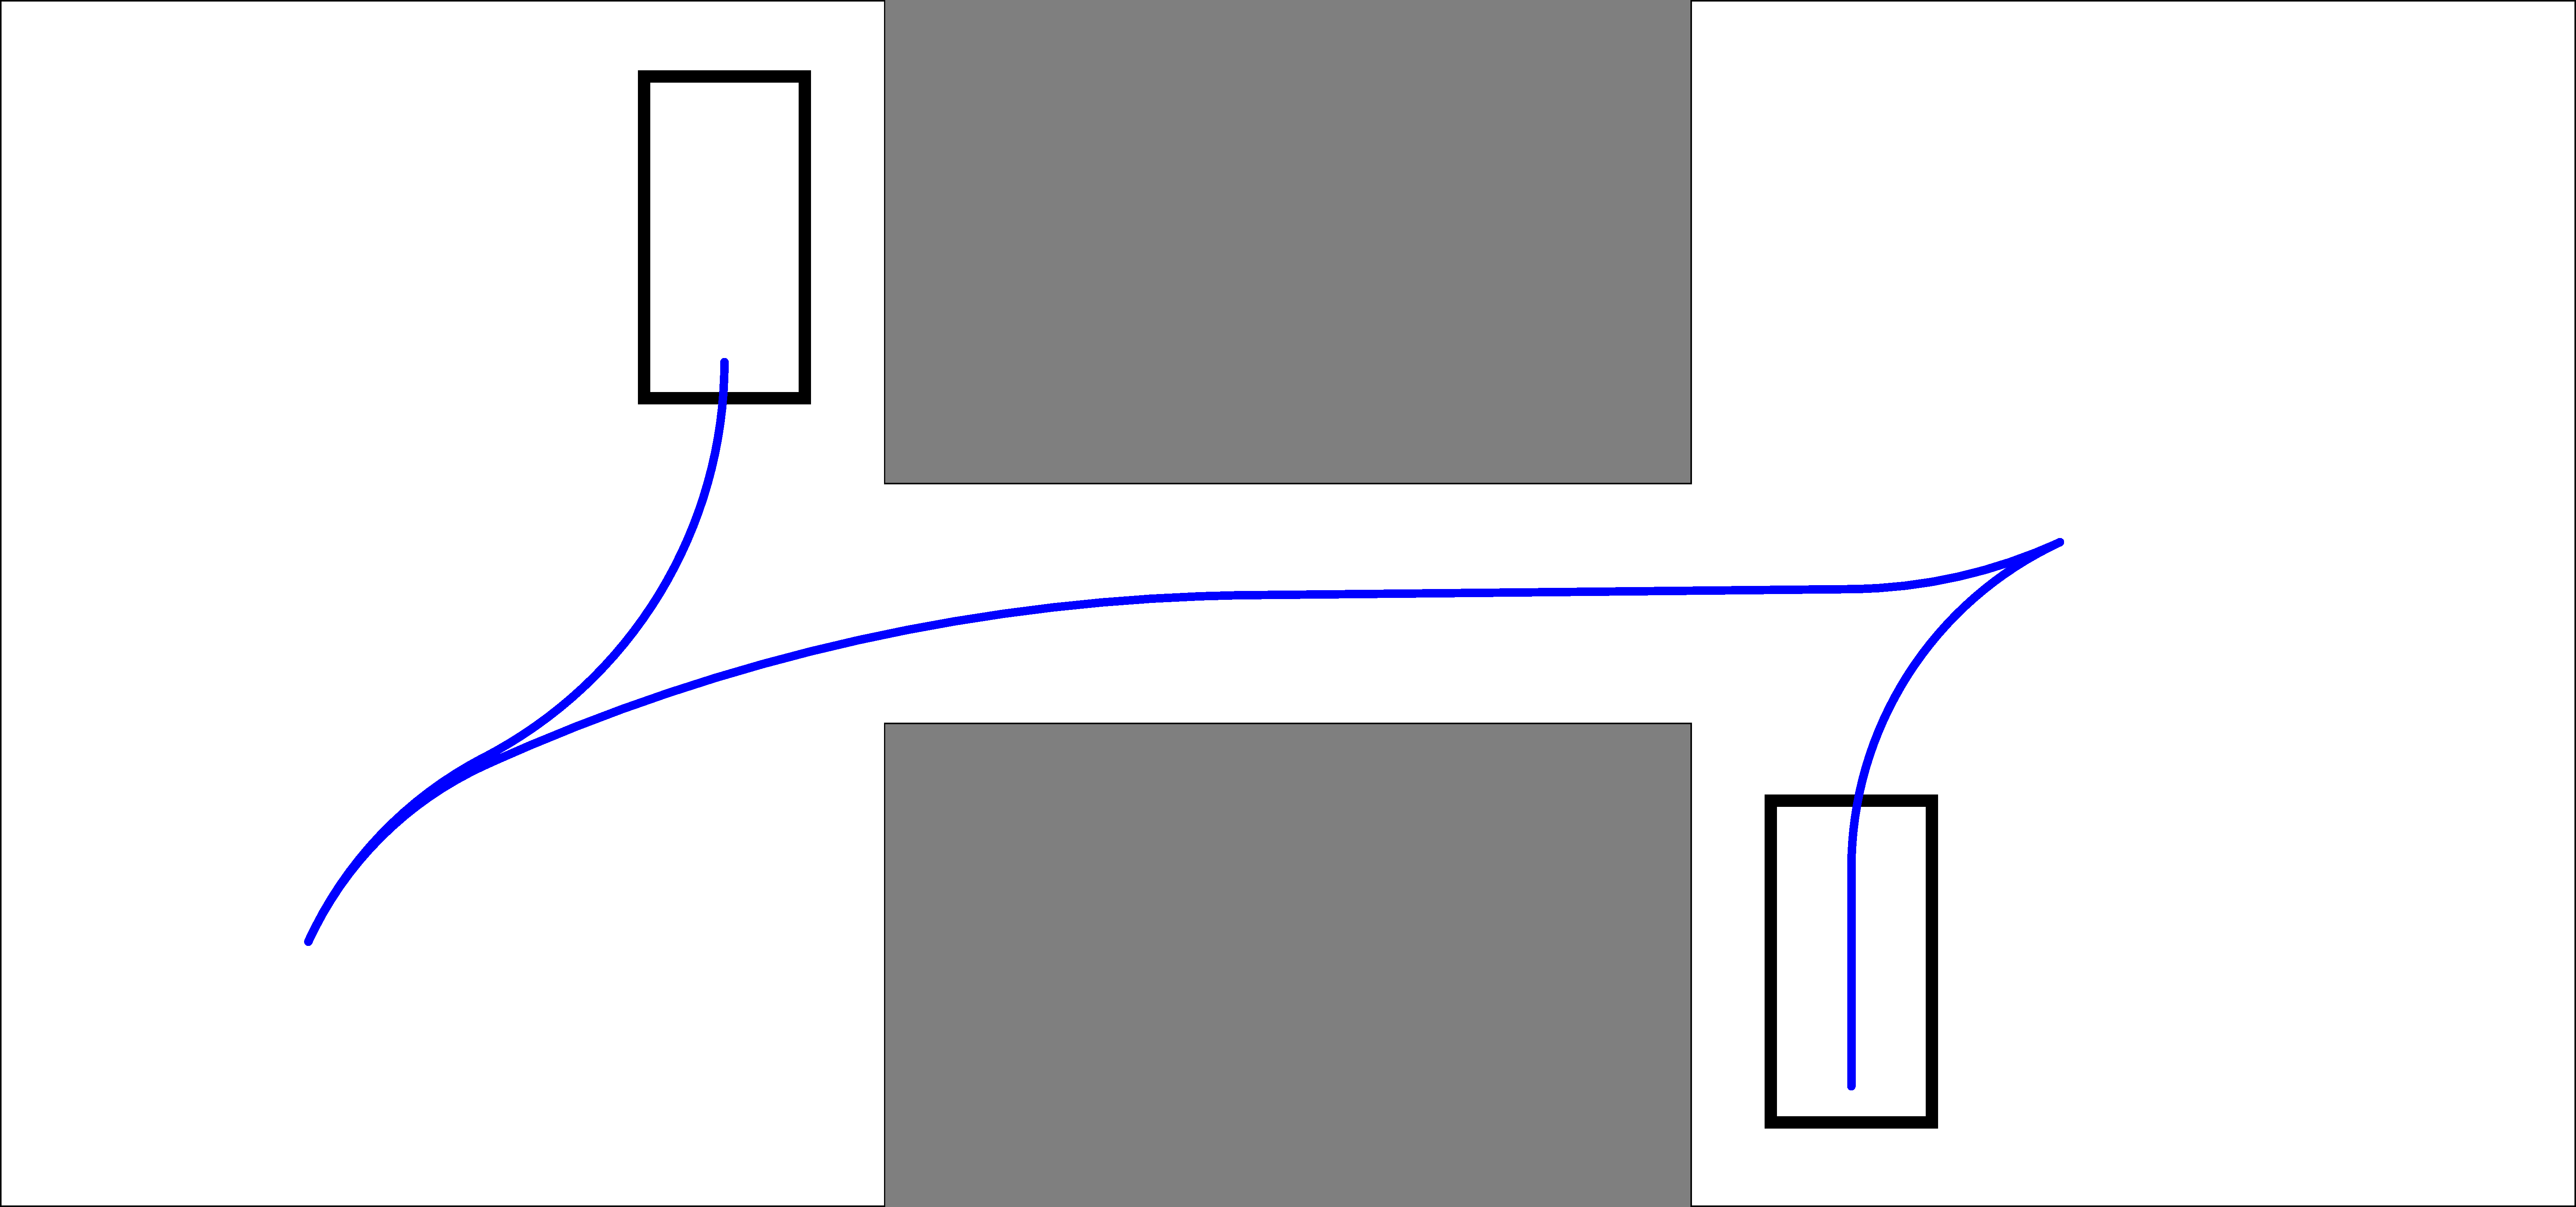
\includegraphics[height=0.35\columnwidth]{.//figures/StaticSim/frame173.pdf}
    \label{subfig:frame173}}}        
    \caption{Four different path between a corridor.}
    \label{fig:staticFrame1}
\end{figure}

\section{Conclusions and Future Work}
\label{sec:conclusions}

We have presented a global geometric path planning method for car-like robots and an analysis about the possible improvements. The RTR path planner with the $C^*CS$ steering-method is capable of designing paths even among obstacles and narrow spaces. The simulation results showed that our planning algorithm can be applied in an unobserved scenarios and the obtained paths are quite ``natural''. Furthermore, it is running time ranges at most a couple of seconds, which makes it feasible for application in real-life situations.

Our future work includes a comprehensive testing on real robot platforms which should verify that these algorithms are well-suited for problems requiring autonomous manoeuvring. A further improvement of the path planner algorithm is in progress, which has the goal of generating paths with continuous curvature.

% conference papers do not normally have an appendix



% use section* for acknowledgement
\section*{Acknowledgement}

This work was partially supported by the European Union and the European Social Fund through project FuturICT.hu (grant no.: TAMOP-4.2.2.C-11/1/KONV-2012-0013) organized by VIKING Zrt. Balatonf\"ured.
This work was partially supported by the Hungarian Government, managed by the National Development Agency, and financed by the Research and Technology Innovation Fond through project eAutoTech (grant no.: KMR\_12-1-2012-0188).






% trigger a \newpage just before the given reference
% number - used to balance the columns on the last page
% adjust value as needed - may need to be readjusted if
% the document is modified later
%\IEEEtriggeratref{8}
% The "triggered" command can be changed if desired:
%\IEEEtriggercmd{\enlargethispage{-5in}}

% references section

% can use a bibliography generated by BibTeX as a .bbl file
% BibTeX documentation can be easily obtained at:
% http://www.ctan.org/tex-archive/biblio/bibtex/contrib/doc/
% The IEEEtran BibTeX style support page is at:
% http://www.michaelshell.org/tex/ieeetran/bibtex/
\bibliographystyle{IEEEtran}
% argument is your BibTeX string definitions and bibliography database(s)
\bibliography{.//bib/IEEEabrv,.//bib/domikiss_ref,.//bib/domikiss_own}





% that's all folks
\end{document}



